
%%
%% This is file `sample-acmsmall-conf.tex',
%% generated with the docstrip utility.
%%
%% The original source files were:
%%
%% samples.dtx  (with options: `all,proceedings,bibtex,acmsmall-conf')
%% 
%% IMPORTANT NOTICE:
%% 
%% For the copyright see the source file.
%% 
%% Any modified versions of this file must be renamed
%% with new filenames distinct from sample-acmsmall-conf.tex.
%% 
%% For distribution of the original source see the terms
%% for copying and modification in the file samples.dtx.
%% 
%% This generated file may be distributed as long as the
%% original source files, as listed above, are part of the
%% same distribution. (The sources need not necessarily be
%% in the same archive or directory.)
%%
%%
%% Commands for TeXCount
%TC:macro \cite [option:text,text]
%TC:macro \citep [option:text,text]
%TC:macro \citet [option:text,text]
%TC:envir table 0 1
%TC:envir table* 0 1
%TC:envir tabular [ignore] word
%TC:envir displaymath 0 word
%TC:envir math 0 word
%TC:envir comment 0 0
%%
%% The first command in your LaTeX source must be the \documentclass
%% command.
%%
%% For submission and review of your manuscript please change the
%% command to \documentclass[manuscript, screen, review]{acmart}.
%%
%% When submitting camera ready or to TAPS, please change the command
%% to \documentclass[sigconf]{acmart} or whichever template is required
%% for your publication.
%%
%%
\documentclass[acmsmall]{acmart}
%%
%% \BibTeX command to typeset BibTeX logo in the docs
\AtBeginDocument{%
  \providecommand\BibTeX{{%
    Bib\TeX}}}

\usepackage{booktabs}
\usepackage{tabularx}
\usepackage{makecell}
%% Rights management information.  This information is sent to you
%% when you complete the rights form.  These commands have SAMPLE
%% values in them; it is your responsibility as an author to replace
%% the commands and values with those provided to you when you
%% complete the rights form.
\setcopyright{acmlicensed}
\copyrightyear{2018}
\acmYear{2018}
\acmDOI{XXXXXXX.XXXXXXX}

%% These commands are for a PROCEEDINGS abstract or paper.
\acmConference[Conference acronym 'XX]{Make sure to enter the correct
  conference title from your rights confirmation email}{June 03--05,
  2018}{Woodstock, NY}
%%
%%  Uncomment \acmBooktitle if the title of the proceedings is different
%%  from ``Proceedings of ...''!
%%
%%\acmBooktitle{Woodstock '18: ACM Symposium on Neural Gaze Detection,
%%  June 03--05, 2018, Woodstock, NY}
\acmISBN{978-1-4503-XXXX-X/2018/06}


%%
%% Submission ID.
%% Use this when submitting an article to a sponsored event. You'll
%% receive a unique submission ID from the organizers
%% of the event, and this ID should be used as the parameter to this command.
%%\acmSubmissionID{123-A56-BU3}

%%
%% For managing citations, it is recommended to use bibliography
%% files in BibTeX format.
%%
%% You can then either use BibTeX with the ACM-Reference-Format style,
%% or BibLaTeX with the acmnumeric or acmauthoryear sytles, that include
%% support for advanced citation of software artefact from the
%% biblatex-software package, also separately available on CTAN.
%%
%% Look at the sample-*-biblatex.tex files for templates showcasing
%% the biblatex styles.
%%

%%
%% The majority of ACM publications use numbered citations and
%% references.  The command \citestyle{authoryear} switches to the
%% "author year" style.
%%
%% If you are preparing content for an event
%% sponsored by ACM SIGGRAPH, you must use the "author year" style of
%% citations and references.
%% Uncommenting
%% the next command will enable that style.



%%
%% end of the preamble, start of the body of the document source.
\begin{document}

%%
%% The "title" command has an optional parameter,
%% allowing the author to define a "short title" to be used in page headers.

%%
%% The "author" command and its associated commands are used to define
%% the authors and their affiliations.
%% Of note is the shared affiliation of the first two authors, and the
%% "authornote" and "authornotemark" commands
%% used to denote shared contribution to the research.
% \author{Ben Trovato}
% \authornote{Both authors contributed equally to this research.}
% \email{trovato@corporation.com}
% \orcid{1234-5678-9012}
% \author{G.K.M. Tobin}
% \authornotemark[1]
% \email{webmaster@marysville-ohio.com}
% \affiliation{%
%   \institution{Institute for Clarity in Documentation}
%   \city{Dublin}
%   \state{Ohio}
%   \country{USA}
% }

% \author{Lars Th{\o}rv{\"a}ld}
% \affiliation{%
%   \institution{The Th{\o}rv{\"a}ld Group}
%   \city{Hekla}
%   \country{Iceland}}
% \email{larst@affiliation.org}

% \author{Valerie B\'eranger}
% \affiliation{%
%   \institution{Inria Paris-Rocquencourt}
%   \city{Rocquencourt}
%   \country{France}
% }

% \author{Aparna Patel}
% \affiliation{%
%  \institution{Rajiv Gandhi University}
%  \city{Doimukh}
%  \state{Arunachal Pradesh}
%  \country{India}}

% \author{Huifen Chan}
% \affiliation{%
%   \institution{Tsinghua University}
%   \city{Haidian Qu}
%   \state{Beijing Shi}
%   \country{China}}

% \author{Charles Palmer}
% \affiliation{%
%   \institution{Palmer Research Laboratories}
%   \city{San Antonio}
%   \state{Texas}
%   \country{USA}}
% \email{cpalmer@prl.com}

% \author{John Smith}
% \affiliation{%
%   \institution{The Th{\o}rv{\"a}ld Group}
%   \city{Hekla}
%   \country{Iceland}}
% \email{jsmith@affiliation.org}

% \author{Julius P. Kumquat}
% \affiliation{%
%   \institution{The Kumquat Consortium}
%   \city{New York}
%   \country{USA}}
% \email{jpkumquat@consortium.net}

% %%
% %% By default, the full list of authors will be used in the page
% %% headers. Often, this list is too long, and will overlap
% %% other information printed in the page headers. This command allows
% %% the author to define a more concise list
% %% of authors' names for this purpose.
% \renewcommand{\shortauthors}{Trovato et al.}

% %%
% %% The abstract is a short summary of the work to be presented in the
% %% article.
% \begin{abstract}
%   A clear and well-documented \LaTeX\ document is presented as an
%   article formatted for publication by ACM in a conference proceedings
%   or journal publication. Based on the ``acmart'' document class, this
%   article presents and explains many of the common variations, as well
%   as many of the formatting elements an author may use in the
%   preparation of the documentation of their work.
% \end{abstract}

% %%
% %% The code below is generated by the tool at http://dl.acm.org/ccs.cfm.
% %% Please copy and paste the code instead of the example below.
% %%
% \begin{CCSXML}
% <ccs2012>
%  <concept>
%   <concept_id>00000000.0000000.0000000</concept_id>
%   <concept_desc>Do Not Use This Code, Generate the Correct Terms for Your Paper</concept_desc>
%   <concept_significance>500</concept_significance>
%  </concept>
%  <concept>
%   <concept_id>00000000.00000000.00000000</concept_id>
%   <concept_desc>Do Not Use This Code, Generate the Correct Terms for Your Paper</concept_desc>
%   <concept_significance>300</concept_significance>
%  </concept>
%  <concept>
%   <concept_id>00000000.00000000.00000000</concept_id>
%   <concept_desc>Do Not Use This Code, Generate the Correct Terms for Your Paper</concept_desc>
%   <concept_significance>100</concept_significance>
%  </concept>
%  <concept>
%   <concept_id>00000000.00000000.00000000</concept_id>
%   <concept_desc>Do Not Use This Code, Generate the Correct Terms for Your Paper</concept_desc>
%   <concept_significance>100</concept_significance>
%  </concept>
% </ccs2012>
% \end{CCSXML}

% \ccsdesc[500]{Do Not Use This Code~Generate the Correct Terms for Your Paper}
% \ccsdesc[300]{Do Not Use This Code~Generate the Correct Terms for Your Paper}
% \ccsdesc{Do Not Use This Code~Generate the Correct Terms for Your Paper}
% \ccsdesc[100]{Do Not Use This Code~Generate the Correct Terms for Your Paper}

% %%
% %% Keywords. The author(s) should pick words that accurately describe
% %% the work being presented. Separate the keywords with commas.
% \keywords{Do, Not, Us, This, Code, Put, the, Correct, Terms, for,
%   Your, Paper}
% %% A "teaser" image appears between the author and affiliation
% %% information and the body of the document, and typically spans the
% %% page.
% \begin{teaserfigure}
%   \includegraphics[width=\textwidth]{sampleteaser}
%   \caption{Seattle Mariners at Spring Training, 2010.}
%   \Description{Enjoying the baseball game from the third-base
%   seats. Ichiro Suzuki preparing to bat.}
%   \label{fig:teaser}
% \end{teaserfigure}

% \received{20 February 2007}
% \received[revised]{12 March 2009}
% \received[accepted]{5 June 2009}

% %%
% %% This command processes the author and affiliation and title
% %% information and builds the first part of the formatted document.
% \maketitle

% \section{Introduction}
% ACM's consolidated article template, introduced in 2017, provides a
% consistent \LaTeX\ style for use across ACM publications, and
% incorporates accessibility and metadata-extraction functionality
% necessary for future Digital Library endeavors. Numerous ACM and
% SIG-specific \LaTeX\ templates have been examined, and their unique
% features incorporated into this single new template.

% If you are new to publishing with ACM, this document is a valuable
% guide to the process of preparing your work for publication. If you
% have published with ACM before, this document provides insight and
% instruction into more recent changes to the article template.

% The ``\verb|acmart|'' document class can be used to prepare articles
% for any ACM publication --- conference or journal, and for any stage
% of publication, from review to final ``camera-ready'' copy, to the
% author's own version, with {\itshape very} few changes to the source.

% \section{Template Overview}
% As noted in the introduction, the ``\verb|acmart|'' document class can
% be used to prepare many different kinds of documentation --- a
% double-anonymous initial submission of a full-length technical paper, a
% two-page SIGGRAPH Emerging Technologies abstract, a ``camera-ready''
% journal article, a SIGCHI Extended Abstract, and more --- all by
% selecting the appropriate {\itshape template style} and {\itshape
%   template parameters}.

% This document will explain the major features of the document
% class. For further information, the {\itshape \LaTeX\ User's Guide} is
% available from
% \url{https://www.acm.org/publications/proceedings-template}.

% \subsection{Template Styles}

% The primary parameter given to the ``\verb|acmart|'' document class is
% the {\itshape template style} which corresponds to the kind of publication
% or SIG publishing the work. This parameter is enclosed in square
% brackets and is a part of the {\verb|documentclass|} command:
% \begin{verbatim}
%   \documentclass[STYLE]{acmart}
% \end{verbatim}

% Journals use one of three template styles. All but three ACM journals
% use the {\verb|acmsmall|} template style:
% \begin{itemize}
% \item {\texttt{acmsmall}}: The default journal template style.
% \item {\texttt{acmlarge}}: Used by JOCCH and TAP.
% \item {\texttt{acmtog}}: Used by TOG.
% \end{itemize}

% The majority of conference proceedings documentation will use the {\verb|acmconf|} template style.
% \begin{itemize}
% \item {\texttt{sigconf}}: The default proceedings template style.
% \item{\texttt{sigchi}}: Used for SIGCHI conference articles.
% \item{\texttt{sigplan}}: Used for SIGPLAN conference articles.
% \end{itemize}

% \subsection{Template Parameters}

% In addition to specifying the {\itshape template style} to be used in
% formatting your work, there are a number of {\itshape template parameters}
% which modify some part of the applied template style. A complete list
% of these parameters can be found in the {\itshape \LaTeX\ User's Guide.}

% Frequently-used parameters, or combinations of parameters, include:
% \begin{itemize}
% \item {\texttt{anonymous,review}}: Suitable for a ``double-anonymous''
%   conference submission. Anonymizes the work and includes line
%   numbers. Use with the \texttt{\string\acmSubmissionID} command to print the
%   submission's unique ID on each page of the work.
% \item{\texttt{authorversion}}: Produces a version of the work suitable
%   for posting by the author.
% \item{\texttt{screen}}: Produces colored hyperlinks.
% \end{itemize}

% This document uses the following string as the first command in the
% source file:
% \begin{verbatim}
% \documentclass[acmsmall]{acmart}
% \end{verbatim}

% \section{Modifications}

% Modifying the template --- including but not limited to: adjusting
% margins, typeface sizes, line spacing, paragraph and list definitions,
% and the use of the \verb|\vspace| command to manually adjust the
% vertical spacing between elements of your work --- is not allowed.

% {\bfseries Your document will be returned to you for revision if
%   modifications are discovered.}

% \section{Typefaces}

% The ``\verb|acmart|'' document class requires the use of the
% ``Libertine'' typeface family. Your \TeX\ installation should include
% this set of packages. Please do not substitute other typefaces. The
% ``\verb|lmodern|'' and ``\verb|ltimes|'' packages should not be used,
% as they will override the built-in typeface families.

% \section{Title Information}

% The title of your work should use capital letters appropriately -
% \url{https://capitalizemytitle.com/} has useful rules for
% capitalization. Use the {\verb|title|} command to define the title of
% your work. If your work has a subtitle, define it with the
% {\verb|subtitle|} command.  Do not insert line breaks in your title.

% If your title is lengthy, you must define a short version to be used
% in the page headers, to prevent overlapping text. The \verb|title|
% command has a ``short title'' parameter:
% \begin{verbatim}
%   \title[short title]{full title}
% \end{verbatim}

% \section{Authors and Affiliations}

% Each author must be defined separately for accurate metadata
% identification.  As an exception, multiple authors may share one
% affiliation. Authors' names should not be abbreviated; use full first
% names wherever possible. Include authors' e-mail addresses whenever
% possible.

% Grouping authors' names or e-mail addresses, or providing an ``e-mail
% alias,'' as shown below, is not acceptable:
% \begin{verbatim}
%   \author{Brooke Aster, David Mehldau}
%   \email{dave,judy,steve@university.edu}
%   \email{firstname.lastname@phillips.org}
% \end{verbatim}

% The \verb|authornote| and \verb|authornotemark| commands allow a note
% to apply to multiple authors --- for example, if the first two authors
% of an article contributed equally to the work.

% If your author list is lengthy, you must define a shortened version of
% the list of authors to be used in the page headers, to prevent
% overlapping text. The following command should be placed just after
% the last \verb|\author{}| definition:
% \begin{verbatim}
%   \renewcommand{\shortauthors}{McCartney, et al.}
% \end{verbatim}
% Omitting this command will force the use of a concatenated list of all
% of the authors' names, which may result in overlapping text in the
% page headers.

% The article template's documentation, available at
% \url{https://www.acm.org/publications/proceedings-template}, has a
% complete explanation of these commands and tips for their effective
% use.

% Note that authors' addresses are mandatory for journal articles.

% \section{Rights Information}

% Authors of any work published by ACM will need to complete a rights
% form. Depending on the kind of work, and the rights management choice
% made by the author, this may be copyright transfer, permission,
% license, or an OA (open access) agreement.

% Regardless of the rights management choice, the author will receive a
% copy of the completed rights form once it has been submitted. This
% form contains \LaTeX\ commands that must be copied into the source
% document. When the document source is compiled, these commands and
% their parameters add formatted text to several areas of the final
% document:
% \begin{itemize}
% \item the ``ACM Reference Format'' text on the first page.
% \item the ``rights management'' text on the first page.
% \item the conference information in the page header(s).
% \end{itemize}

% Rights information is unique to the work; if you are preparing several
% works for an event, make sure to use the correct set of commands with
% each of the works.

% The ACM Reference Format text is required for all articles over one
% page in length, and is optional for one-page articles (abstracts).

% \section{CCS Concepts and User-Defined Keywords}

% Two elements of the ``acmart'' document class provide powerful
% taxonomic tools for you to help readers find your work in an online
% search.

% The ACM Computing Classification System ---
% \url{https://www.acm.org/publications/class-2012} --- is a set of
% classifiers and concepts that describe the computing
% discipline. Authors can select entries from this classification
% system, via \url{https://dl.acm.org/ccs/ccs.cfm}, and generate the
% commands to be included in the \LaTeX\ source.

% User-defined keywords are a comma-separated list of words and phrases
% of the authors' choosing, providing a more flexible way of describing
% the research being presented.

% CCS concepts and user-defined keywords are required for for all
% articles over two pages in length, and are optional for one- and
% two-page articles (or abstracts).

% \section{Sectioning Commands}

% Your work should use standard \LaTeX\ sectioning commands:
% \verb|\section|, \verb|\subsection|, \verb|\subsubsection|,
% \verb|\paragraph|, and \verb|\subparagraph|. The sectioning levels up to
% \verb|\subsusection| should be numbered; do not remove the numbering
% from the commands.

% Simulating a sectioning command by setting the first word or words of
% a paragraph in boldface or italicized text is {\bfseries not allowed.}

% Below are examples of sectioning commands.

% \subsection{Subsection}
% \label{sec:subsection}

% This is a subsection.

% \subsubsection{Subsubsection}
% \label{sec:subsubsection}

% This is a subsubsection.

% \paragraph{Paragraph}

% This is a paragraph.

% \subparagraph{Subparagraph}

% This is a subparagraph.

% \section{Tables}

% The ``\verb|acmart|'' document class includes the ``\verb|booktabs|''
% package --- \url{https://ctan.org/pkg/booktabs} --- for preparing
% high-quality tables.

% Table captions are placed {\itshape above} the table.

% Because tables cannot be split across pages, the best placement for
% them is typically the top of the page nearest their initial cite.  To
% ensure this proper ``floating'' placement of tables, use the
% environment \textbf{table} to enclose the table's contents and the
% table caption.  The contents of the table itself must go in the
% \textbf{tabular} environment, to be aligned properly in rows and
% columns, with the desired horizontal and vertical rules.  Again,
% detailed instructions on \textbf{tabular} material are found in the
% \paragraph{\LaTeX\ User's Guide}.

% Immediately following this sentence is the point at which
% Table~\ref{tab:freq} is included in the input file; compare the
% placement of the table here with the table in the printed output of
% this document.

% \begin{table}
%   \caption{Frequency of Special Characters}
%   \label{tab:freq}
%   \begin{tabular}{ccl}
%     \toprule
%     Non-English or Math&Frequency&Comments\\
%     \midrule
%     \O & 1 in 1,000& For Swedish names\\
%     $\pi$ & 1 in 5& Common in math\\
%     \$ & 4 in 5 & Used in business\\
%     $\Psi^2_1$ & 1 in 40,000& Unexplained usage\\
%   \bottomrule
% \end{tabular}
% \end{table}

% To set a wider table, which takes up the whole width of the page's
% live area, use the environment \textbf{table*} to enclose the table's
% contents and the table caption.  As with a single-column table, this
% wide table will ``float'' to a location deemed more
% desirable. Immediately following this sentence is the point at which
% Table~\ref{tab:commands} is included in the input file; again, it is
% instructive to compare the placement of the table here with the table
% in the printed output of this document.

% \begin{table*}
%   \caption{Some Typical Commands}
%   \label{tab:commands}
%   \begin{tabular}{ccl}
%     \toprule
%     Command &A Number & Comments\\
%     \midrule
%     \texttt{{\char'134}author} & 100& Author \\
%     \texttt{{\char'134}table}& 300 & For tables\\
%     \texttt{{\char'134}table*}& 400& For wider tables\\
%     \bottomrule
%   \end{tabular}
% \end{table*}

% Always use midrule to separate table header rows from data rows, and
% use it only for this purpose. This enables assistive technologies to
% recognise table headers and support their users in navigating tables
% more easily.

% \section{Math Equations}
% You may want to display math equations in three distinct styles:
% inline, numbered or non-numbered display.  Each of the three are
% discussed in the next sections.

% \subsection{Inline (In-text) Equations}
% A formula that appears in the running text is called an inline or
% in-text formula.  It is produced by the \textbf{math} environment,
% which can be invoked with the usual
% \texttt{{\char'134}begin\,\ldots{\char'134}end} construction or with
% the short form \texttt{\$\,\ldots\$}. You can use any of the symbols
% and structures, from $\alpha$ to $\omega$, available in
% \LaTeX~\cite{Lamport:LaTeX}; this section will simply show a few
% examples of in-text equations in context. Notice how this equation:
% \begin{math}
%   \lim_{n\rightarrow \infty}x=0
% \end{math},
% set here in in-line math style, looks slightly different when
% set in display style.  (See next section).

% \subsection{Display Equations}
% A numbered display equation---one set off by vertical space from the
% text and centered horizontally---is produced by the \textbf{equation}
% environment. An unnumbered display equation is produced by the
% \textbf{displaymath} environment.

% Again, in either environment, you can use any of the symbols and
% structures available in \LaTeX\@; this section will just give a couple
% of examples of display equations in context.  First, consider the
% equation, shown as an inline equation above:
% \begin{equation}
%   \lim_{n\rightarrow \infty}x=0
% \end{equation}
% Notice how it is formatted somewhat differently in
% the \textbf{displaymath}
% environment.  Now, we'll enter an unnumbered equation:
% \begin{displaymath}
%   \sum_{i=0}^{\infty} x + 1
% \end{displaymath}
% and follow it with another numbered equation:
% \begin{equation}
%   \sum_{i=0}^{\infty}x_i=\int_{0}^{\pi+2} f
% \end{equation}
% just to demonstrate \LaTeX's able handling of numbering.

% \section{Figures}

% The ``\verb|figure|'' environment should be used for figures. One or
% more images can be placed within a figure. If your figure contains
% third-party material, you must clearly identify it as such, as shown
% in the example below.
% \begin{figure}[ht]
%   \centering
%   \includegraphics[width=\linewidth]{sample-franklin}
%   \caption{1907 Franklin Model D roadster. Photograph by Harris \&
%     Ewing, Inc. [Public domain], via Wikimedia
%     Commons. (\url{https://goo.gl/VLCRBB}).}
%   \Description{A woman and a girl in white dresses sit in an open car.}
% \end{figure}

% Your figures should contain a caption which describes the figure to
% the reader.

% Figure captions are placed {\itshape below} the figure.

% Every figure should also have a figure description unless it is purely
% decorative. These descriptions convey what’s in the image to someone
% who cannot see it. They are also used by search engine crawlers for
% indexing images, and when images cannot be loaded.

% A figure description must be unformatted plain text less than 2000
% characters long (including spaces).  {\bfseries Figure descriptions
%   should not repeat the figure caption – their purpose is to capture
%   important information that is not already provided in the caption or
%   the main text of the paper.} For figures that convey important and
% complex new information, a short text description may not be
% adequate. More complex alternative descriptions can be placed in an
% appendix and referenced in a short figure description. For example,
% provide a data table capturing the information in a bar chart, or a
% structured list representing a graph.  For additional information
% regarding how best to write figure descriptions and why doing this is
% so important, please see
% \url{https://www.acm.org/publications/taps/describing-figures/}.

% \subsection{The ``Teaser Figure''}

% A ``teaser figure'' is an image, or set of images in one figure, that
% are placed after all author and affiliation information, and before
% the body of the article, spanning the page. If you wish to have such a
% figure in your article, place the command immediately before the
% \verb|\maketitle| command:
% \begin{verbatim}
%   \begin{teaserfigure}
%     \includegraphics[width=\textwidth]{sampleteaser}
%     \caption{figure caption}
%     \Description{figure description}
%   \end{teaserfigure}
% \end{verbatim}

% \section{Citations and Bibliographies}

% The use of \BibTeX\ for the preparation and formatting of one's
% references is strongly recommended. Authors' names should be complete
% --- use full first names (``Donald E. Knuth'') not initials
% (``D. E. Knuth'') --- and the salient identifying features of a
% reference should be included: title, year, volume, number, pages,
% article DOI, etc.

% The bibliography is included in your source document with these two
% commands, placed just before the \verb|\end{document}| command:
% \begin{verbatim}
%   \bibliographystyle{ACM-Reference-Format}
%   \bibliography{bibfile}
% \end{verbatim}
% where ``\verb|bibfile|'' is the name, without the ``\verb|.bib|''
% suffix, of the \BibTeX\ file.

% Citations and references are numbered by default. A small number of
% ACM publications have citations and references formatted in the
% ``author year'' style; for these exceptions, please include this
% command in the {\bfseries preamble} (before the command
% ``\verb|\begin{document}|'') of your \LaTeX\ source:
% \begin{verbatim}

% \end{verbatim}


%   Some examples.  A paginated journal article \cite{Abril07}, an
%   enumerated journal article \cite{Cohen07}, a reference to an entire
%   issue \cite{JCohen96}, a monograph (whole book) \cite{Kosiur01}, a
%   monograph/whole book in a series (see 2a in spec. document)
%   \cite{Harel79}, a divisible-book such as an anthology or compilation
%   \cite{Editor00} followed by the same example, however we only output
%   the series if the volume number is given \cite{Editor00a} (so
%   Editor00a's series should NOT be present since it has no vol. no.),
%   a chapter in a divisible book \cite{Spector90}, a chapter in a
%   divisible book in a series \cite{Douglass98}, a multi-volume work as
%   book \cite{Knuth97}, a couple of articles in a proceedings (of a
%   conference, symposium, workshop for example) (paginated proceedings
%   article) \cite{Andler79, Hagerup1993}, a proceedings article with
%   all possible elements \cite{Smith10}, an example of an enumerated
%   proceedings article \cite{VanGundy07}, an informally published work
%   \cite{Harel78}, a couple of preprints \cite{Bornmann2019,
%     AnzarootPBM14}, a doctoral dissertation \cite{Clarkson85}, a
%   master's thesis: \cite{anisi03}, an online document / world wide web
%   resource \cite{Thornburg01, Ablamowicz07, Poker06}, a video game
%   (Case 1) \cite{Obama08} and (Case 2) \cite{Novak03} and \cite{Lee05}
%   and (Case 3) a patent \cite{JoeScientist001}, work accepted for
%   publication \cite{rous08}, 'YYYYb'-test for prolific author
%   \cite{SaeediMEJ10} and \cite{SaeediJETC10}. Other cites might
%   contain 'duplicate' DOI and URLs (some SIAM articles)
%   \cite{Kirschmer:2010:AEI:1958016.1958018}. Boris / Barbara Beeton:
%   multi-volume works as books \cite{MR781536} and \cite{MR781537}. A
%   couple of citations with DOIs:
%   \cite{2004:ITE:1009386.1010128,Kirschmer:2010:AEI:1958016.1958018}. Online
%   citations: \cite{TUGInstmem, Thornburg01, CTANacmart}.
%   Artifacts: \cite{R} and \cite{UMassCitations}.

% \section{Acknowledgments}

% Identification of funding sources and other support, and thanks to
% individuals and groups that assisted in the research and the
% preparation of the work should be included in an acknowledgment
% section, which is placed just before the reference section in your
% document.

% This section has a special environment:
% \begin{verbatim}
%   \begin{acks}
%   ...
%   \end{acks}
% \end{verbatim}
% so that the information contained therein can be more easily collected
% during the article metadata extraction phase, and to ensure
% consistency in the spelling of the section heading.

% Authors should not prepare this section as a numbered or unnumbered {\verb|\section|}; please use the ``{\verb|acks|}'' environment.

% \section{Appendices}

% If your work needs an appendix, add it before the
% ``\verb|\end{document}|'' command at the conclusion of your source
% document.

% Start the appendix with the ``\verb|appendix|'' command:
% \begin{verbatim}
%   \appendix
% \end{verbatim}
% and note that in the appendix, sections are lettered, not
% numbered. This document has two appendices, demonstrating the section
% and subsection identification method.

% \section{Multi-language papers}

% Papers may be written in languages other than English or include
% titles, subtitles, keywords and abstracts in different languages (as a
% rule, a paper in a language other than English should include an
% English title and an English abstract).  Use \verb|language=...| for
% every language used in the paper.  The last language indicated is the
% main language of the paper.  For example, a French paper with
% additional titles and abstracts in English and German may start with
% the following command
% \begin{verbatim}
% \documentclass[sigconf, language=english, language=german,
%                language=french]{acmart}
% \end{verbatim}

% The title, subtitle, keywords and abstract will be typeset in the main
% language of the paper.  The commands \verb|\translatedXXX|, \verb|XXX|
% begin title, subtitle and keywords, can be used to set these elements
% in the other languages.  The environment \verb|translatedabstract| is
% used to set the translation of the abstract.  These commands and
% environment have a mandatory first argument: the language of the
% second argument.  See \verb|sample-sigconf-i13n.tex| file for examples
% of their usage.

% \section{SIGCHI Extended Abstracts}

% The ``\verb|sigchi-a|'' template style (available only in \LaTeX\ and
% not in Word) produces a landscape-orientation formatted article, with
% a wide left margin. Three environments are available for use with the
% ``\verb|sigchi-a|'' template style, and produce formatted output in
% the margin:
% \begin{description}
% \item[\texttt{sidebar}:]  Place formatted text in the margin.
% \item[\texttt{marginfigure}:] Place a figure in the margin.
% \item[\texttt{margintable}:] Place a table in the margin.
% \end{description}

% %%
% %% The acknowledgments section is defined using the "acks" environment
% %% (and NOT an unnumbered section). This ensures the proper
% %% identification of the section in the article metadata, and the
% %% consistent spelling of the heading.
% \begin{acks}
% To Robert, for the bagels and explaining CMYK and color spaces.
% \end{acks}

% %%
% %% The next two lines define the bibliography style to be used, and
% %% the bibliography file.






%%
%% The "title" command has an optional parameter,
%% allowing the author to define a "short title" to be used in page headers.
% \title{A Review of DNN-Based Spatiotemporal Models for Digital Health: Toward Digital Twin Integration}
\title{Spatiotemporal Deep Learning for Digital Health: From Predictive Models to Digital Twins and World Models}
%%

\renewcommand{\shortauthors}{Trovato et al.}
%%
%% Article type: Research, Review, Discussion, Invited or position
\acmArticleType{Review}
%%
%% Links to code and data
% \acmCodeLink{https://github.com/borisveytsman/acmart}
% \acmDataLink{htps://zenodo.org/link}
%%
%% Authors' contribution
\acmContributions{1. Developing a digital-health-centered taxonomy that connects spatiotemporal data types, preprocessing challenges, deep neural architectures, and representative clinical applications.
2. Synthesizing sequence, graph, convolutional, transformer, irregular-time, longitudinal, and statistical-deep-learning perspectives to clarify when different model families are appropriate for digital health data.
3. Analyzing deployment pathways for spatiotemporal models through medical digital twins, privacy-preserving federated learning, visualization, uncertainty quantification, and emerging world-model-based patient simulators.}
%%
%% Sometimes the addresses are too long to fit on the page.  In this
%% case uncomment the lines below and fill them accodingly.
%%
%% \authorsaddresses{Corresponding author: Ben Trovato,
%% \href{mailto:trovato@corporation.com}{trovato@corporation.com};
%% Institute for Clarity in Documentation, P.O. Box 1212, Dublin,
%% Ohio, USA, 43017-6221}
%%
%%
%% Keywords. The author(s) should pick words that accurately describe
%% the work being presented. Separate the keywords with commas.

\keywords{Spatiotemporal model, deep neural networks, digital health, longitudinal data, world models, chronic disease}

\begin{abstract}
Human health and disease progression are closely influenced by environmental, behavioral, and spatial factors. However, existing digital health research has largely relied on traditional clinical records, which lack continuous spatiotemporal context and fail to capture environmental and lifestyle exposures. While recent advances in wearable sensing and mobile health technologies enable the collection of rich longitudinal data, existing surveys typically focus on either temporal modeling or isolated data modalities, lacking a unified perspective on spatiotemporal learning in digital health. In this survey, we systematically review recent developments in spatiotemporal modeling for digital health, covering sequence based models, graph based approaches, world model and emerging digital twin frameworks applied to longitudinal health data, environmental exposure, and lifestyle factors such as diet. We categorize existing methods, analyze their design trade-offs, and compare their applicability across different healthcare scenarios. A central theme of our review is that spatiotemporal deep learning supplies the predictive backbone for two increasingly important paradigms: world models, which learn the latent dynamics of a patient's state to support simulation and counterfactual reasoning over candidate interventions, and digital twins, which embed these learned dynamics in a continuously updated virtual representation of an individual. We show how the same spatiotemporal representations that drive health trajectory prediction also enable world models to anticipate how a patient would respond to alternative actions and allow digital twins to keep that simulation synchronized with streaming real world observations. Our analysis reveals that integrating spatial and environmental context consistently improves chronic disease prediction and enables more accurate health trajectory modeling, while lifestyle factors remain underutilized despite their strong predictive potential. We further identify key challenges, including data sparsity, heterogeneity, and continuous model updating. These findings highlight the importance of developing continuous, adaptive, and personalized health modeling systems, and suggest that future research could focus on real time data integration, world model based and digital twin driven simulation, and privacy preserving learning for scalable healthcare applications.

\end{abstract}

\begin{CCSXML}
<ccs2012>
<concept>
<concept_id>10010147.10010178</concept_id>
<concept_desc>Computing methodologies~Artificial intelligence</concept_desc>
<concept_significance>500</concept_significance>
</concept>
</ccs2012>
\end{CCSXML}

\ccsdesc[500]{Computing methodologies~Artificial intelligence}

\maketitle

% \begin{figure}[ht]
%     \centering
%     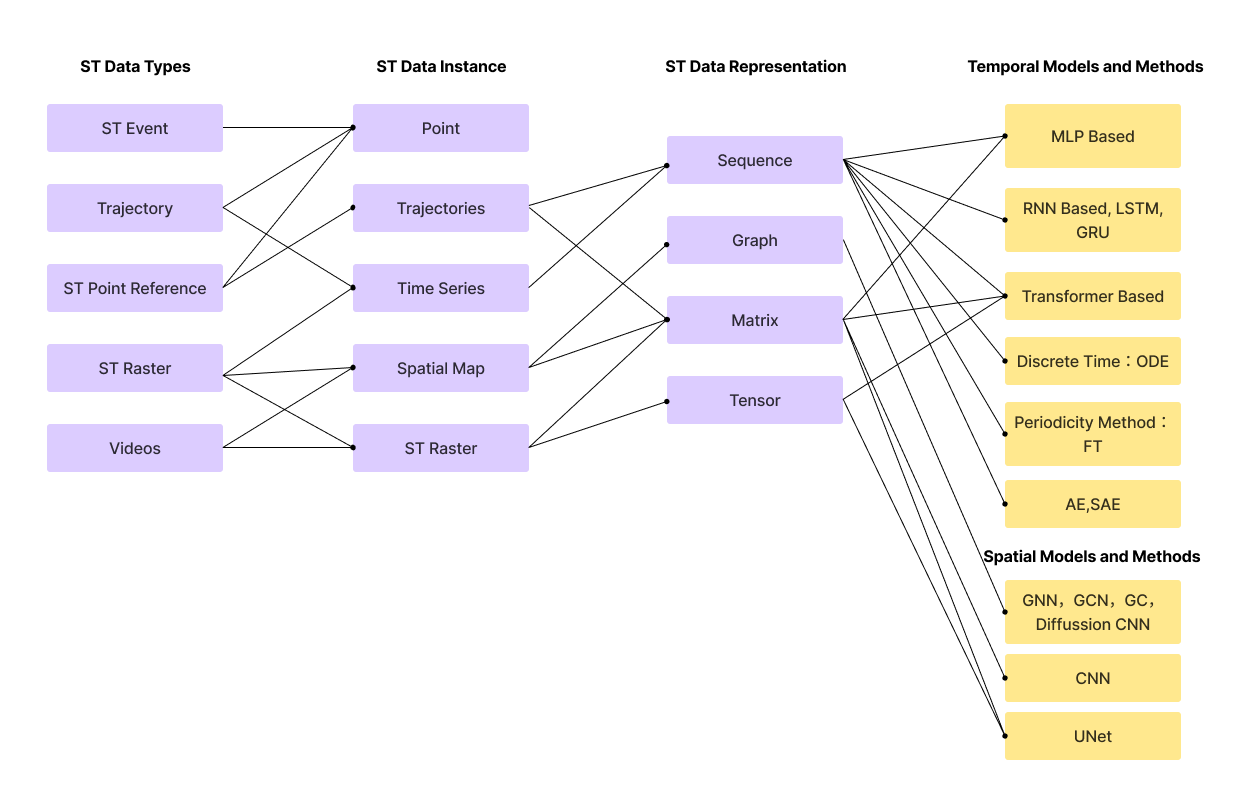
\includegraphics[width=\linewidth]{Frame 9 (3).png}
%     \caption{ST Data Categories}
%     \Description{A diagram illustrating different categories of Spatiotemporaldata (e.g., spatial only, temporal only, Spatiotemporal).}

%     \label{fig:ST Data Categories}
% \end{figure}


\section{Introduction}
When patients seek care, clinicians typically combine static patient characteristics, snapshot clinical observations, demographic risk factors, and longitudinal history such as prior diagnoses, laboratory trends, medication records, and treatment responses. Static information helps assign patients to broad risk groups, snapshot observations indicate the current clinical state, and historical records provide temporal context for understanding disease progression. For chronic or progressive diseases, periodic follow-up visits create an intermittently sampled view of health evolution, but this view remains coarse, fragmented, and often disconnected from daily behavior and environmental exposure. Digital health reframes this workflow as a collection of time-stamped and context-dependent observations, enabling symptoms, physiological signals, behavioral patterns, and exposures to be recorded more continuously and modeled as evolving trajectories.

Computational health modeling has gradually moved from static risk estimation toward dynamic and contextual prediction. Early rule-based systems were interpretable but struggled with ambiguity, incomplete information, and heterogeneity across patients. Electronic health records enabled probabilistic and survival models for population-level risk prediction, while later machine learning methods improved nonlinear pattern recognition but often reduced longitudinal history to aggregated features. A major shift occurred when temporal models began to represent disease evolution directly from sequential observations, a transition accelerated by wearable sensors and mobile health technologies. In diabetes management, for example, models trained on continuous glucose monitoring data can capture short-term glucose dynamics and longer-term changes in insulin sensitivity, supporting more responsive prediction and treatment adjustment \cite{Vaughan2025CGMPrediction,Gecili2020CGMPrediction}.

Temporal modeling alone, however, cannot fully represent how health unfolds in real life. Human health evolves in a four-dimensional setting shaped by time and space: geographic location, food environments, air quality, physical activity opportunities, mobility patterns, work routines, and socioeconomic context all influence physiological and behavioral trajectories. Large-scale nutrition studies, for instance, show that diet quality and chronic disease risk vary systematically across regions and socioeconomic groups \cite{McCullough2022Diet}. Incorporating spatial information therefore allows models to connect environmental and lifestyle context with longitudinal patient states, improving personalization and helping explain why individuals with similar clinical profiles may follow different health trajectories.


\begin{figure}
    \centering
    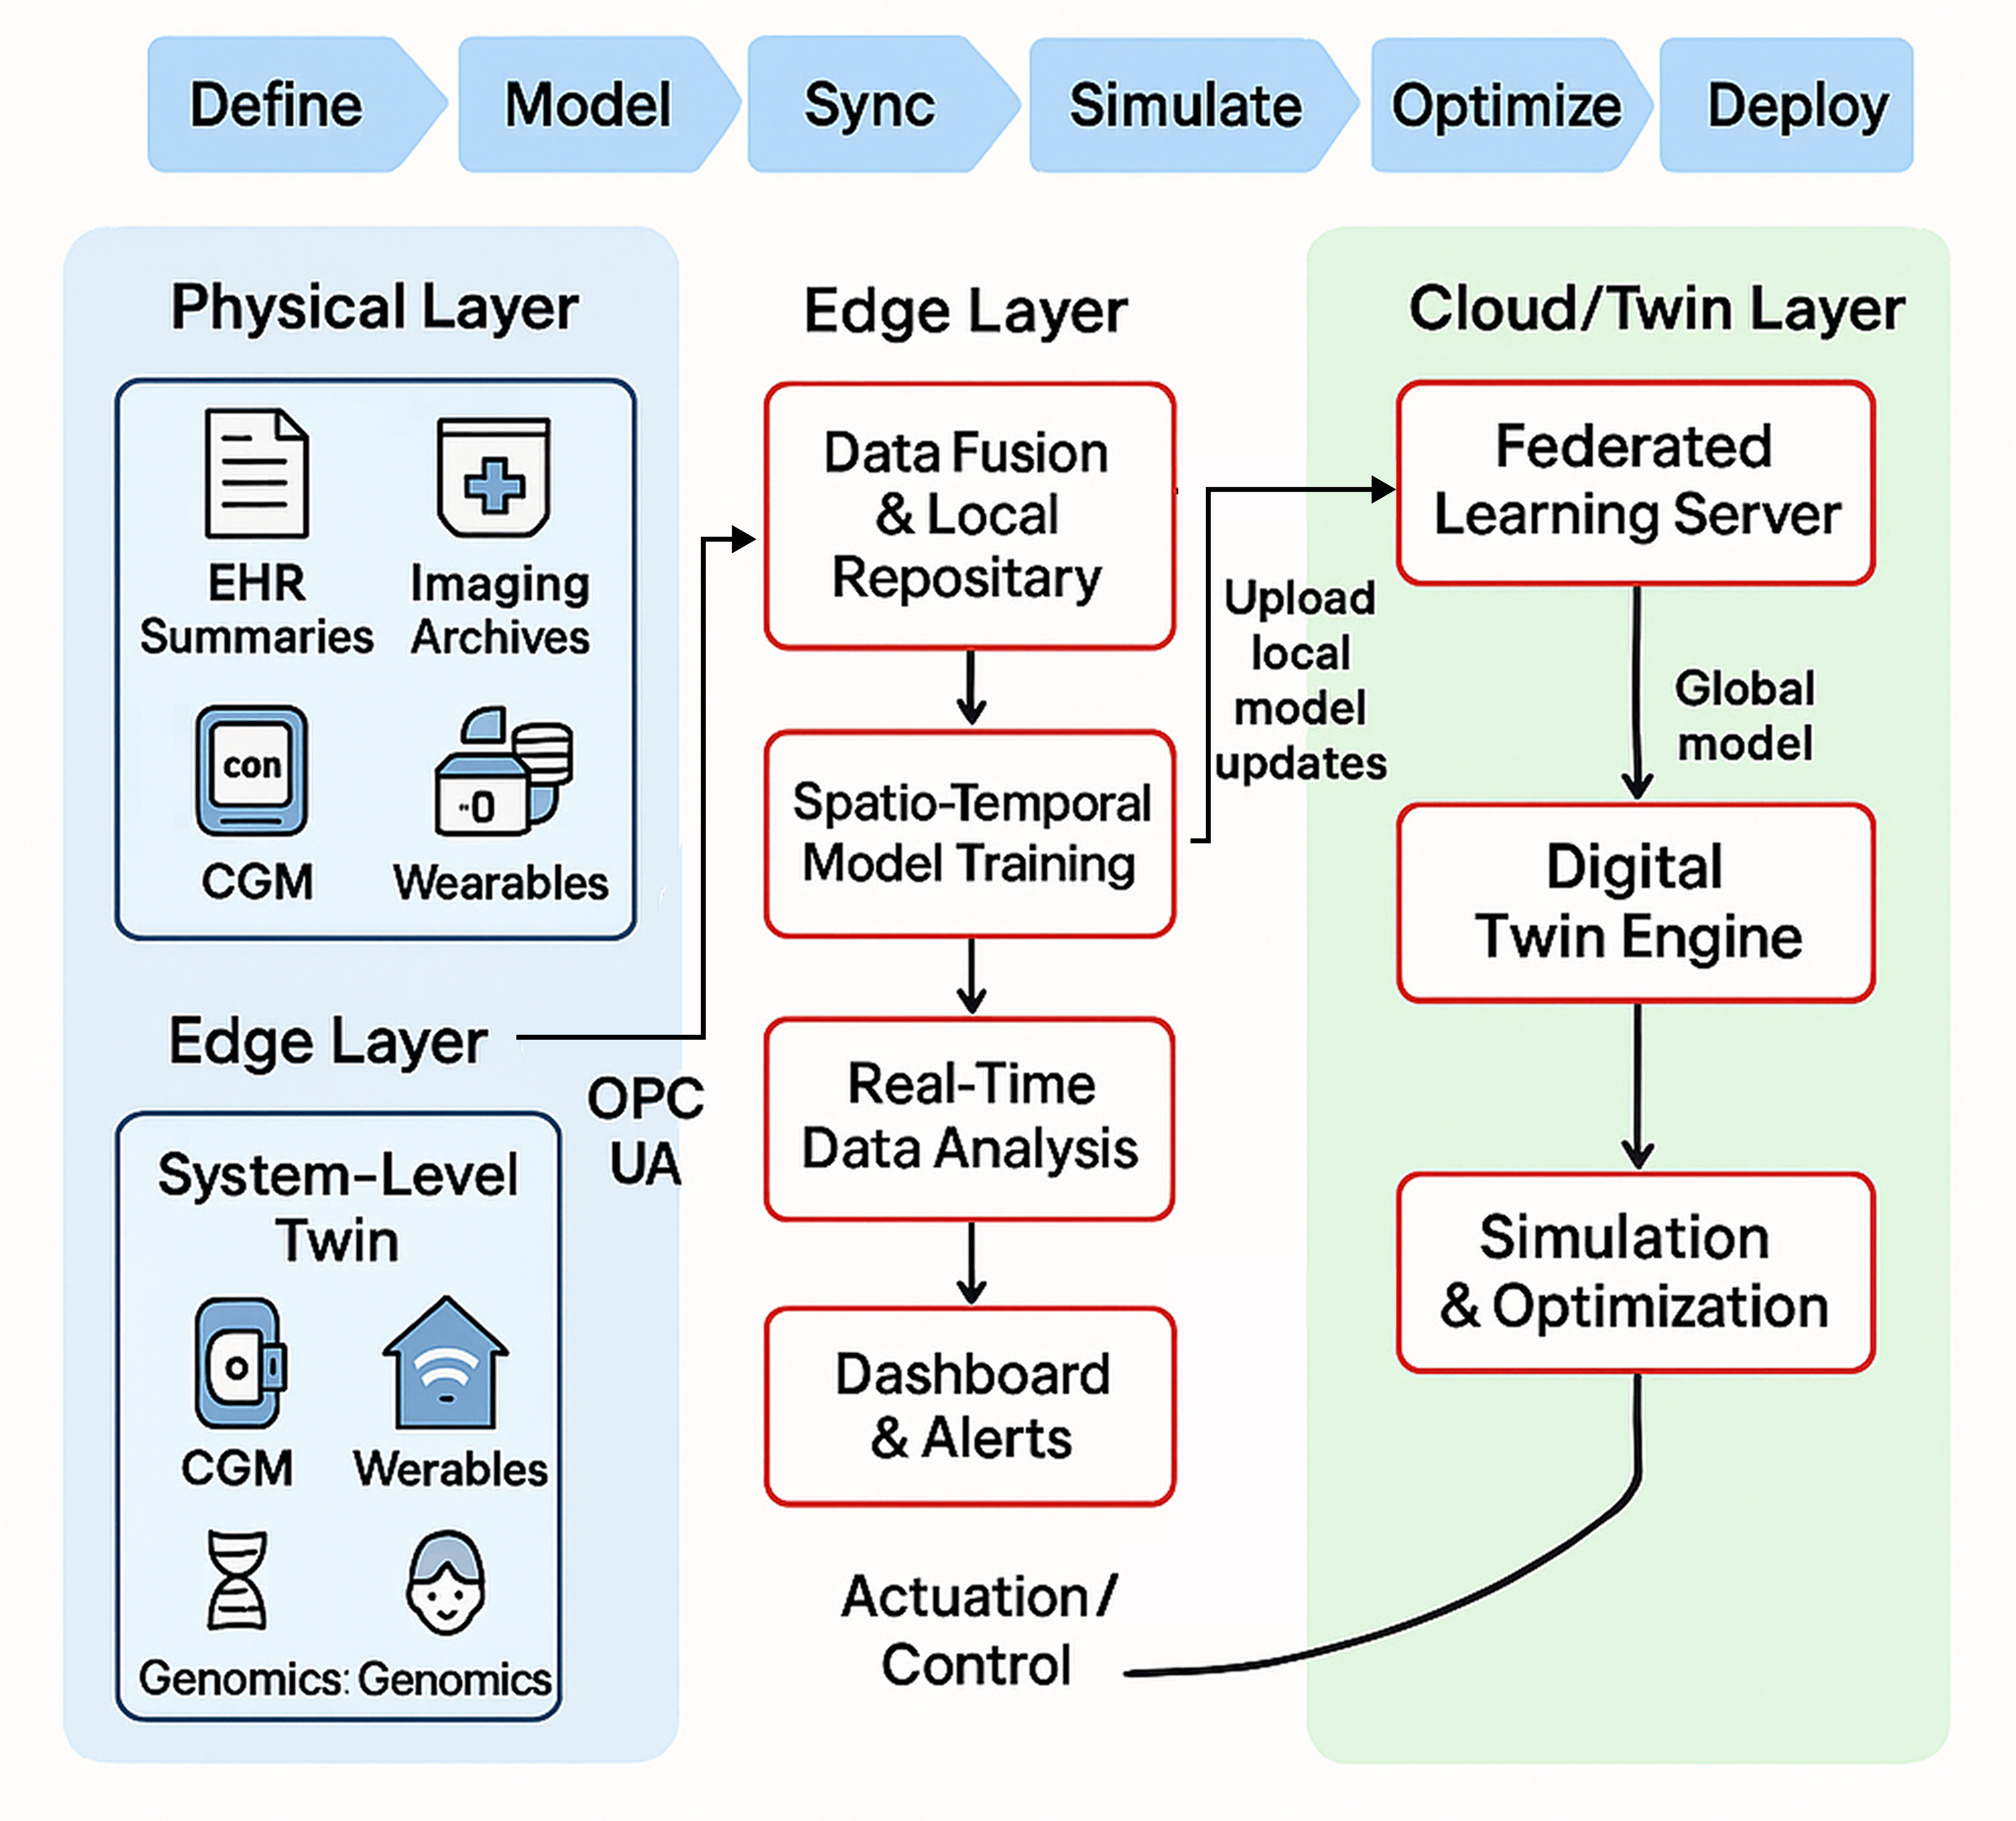
\includegraphics[width=0.75\linewidth]{digital twin in health care.png}
    \caption{Conceptual overview of a digital twin in healthcare: real world patient data from sensors, wearables, and clinical records continuously update a virtual patient replica, which in turn supports monitoring, prediction, and intervention planning in a closed feedback loop.}
    \Description{A conceptual diagram of a digital twin in healthcare, in which real world patient data from sensors, wearables, and clinical records continuously update a virtual patient replica that supports monitoring, prediction, and intervention planning.}
    \label{fig:digital twin in health care}
\end{figure}
This survey argues that spatiotemporal modeling is a necessary step in this progression. By reviewing spatiotemporal models and their applications in digital health, we aim to clarify how environmental and lifestyle factors such as dietary quality can be incorporated into longitudinal disease prediction, and how such models can support more faithful and personalized digital twin systems for healthcare.


Our primary audience comprises (i) developers who build spatiotemporal models (ii) researchers who plan to deploy models in digital‑health settings or digital twin research. To serve these groups, we first introduce a practical taxonomy of spatiotemporal models for digital health; we then explore application scenarios, recommend appropriate data‑processing pipelines and model choices, and provide guidelines for thorough evaluation by comparing different models. We also present representative case studies—including diet‑related chronic‑disease datasets—to illustrate best practices. Finally, we address common privacy concerns that arise during deployment (e.g., patient data protection) and discuss potential solutions such as federated learning, before forecasting future trends in model adoption and the role of digital twin in digital health.

All data used in this study are deidentified and comply with relevant data protection regulations. Data access and usage follow institutional and ethical guidelines. No identifiable personal information is used, and data ownership remains with the original data providers.

First, we develop a digital-health-centered taxonomy that connects spatiotemporal data types (event, trajectory, point-reference, raster, and video data), their preprocessing challenges (sparsity, irregular sampling, and multi-scale spatial and temporal structure), the foundational deep architectures (CNN, GNN, RNN, and Transformer), and representative clinical applications, providing a unified map from data to model to deployment. Second, we synthesize the major spatiotemporal model families---CNN--RNN hybrids, spatiotemporal graph neural networks, Transformer-based models, 3D-CNN and hybrid networks, and irregular-time, longitudinal, and statistical deep-learning approaches---with practical guidance on when each family is appropriate for digital-health data, illustrated across dietary, diabetes, depression, and cardiac applications. Third, we analyze deployment pathways for spatiotemporal models through medical digital twins, including privacy-preserving federated learning, visualization, uncertainty quantification, and emerging world-model-based patient simulators for counterfactual planning. Finally, we present a diet-centered case study on chronic-disease analysis that demonstrates best practices for data processing, model selection, and evaluation, grounding the survey's recommendations in a concrete spatiotemporal digital-health setting.


The remainder of this survey is organized as follows. 
Section~\ref{sec:data} introduces the characteristics of spatiotemporal data in digital health and discusses key challenges such as sparsity, irregular sampling, and multi-scale structures. 
Section~\ref{sec:history} reviews the historical development of deep learning–based spatiotemporal modeling methods.
Section~\ref{sec:models} presents spatiotemporal modeling approaches and their applications in digital health across multiple domains. 
Section~\ref{sec:categorization} further categorizes deep learning–based medical models and longitudinal modeling strategies, providing a unified perspective on existing methodologies.
Section~\ref{sec:DT} discusses the integration of spatiotemporal models within digital twin systems, including modeling, system integration, and key challenges such as data collection and privacy. 
Finally, Section~\ref{sec:future} outlines future research directions and the potential of combining spatiotemporal modeling with digital twin technologies in real-world healthcare applications.


\section{Spatiotemporal Data in Digital Health}
\label{sec:data}
Before introducing spatiotemporal models, it is useful to clarify what we mean by spatiotemporal 
data in the first place. In the physical world, most patient-related phenomena can be indexed by 
both time and space, which means they can often be represented in four dimensions: three spatial 
dimensions plus one temporal dimension. Drawing on prior work~\cite{wang2022deep,atluri2018stdm}, spatiotemporal 
data in digital health can be categorized into five major types: event data, trajectory data, 
point reference data, raster data, and video data, as illustrated in Figure~\ref{fig:Five Spatio temporal Data Categories}.




\begin{figure}
    \centering
    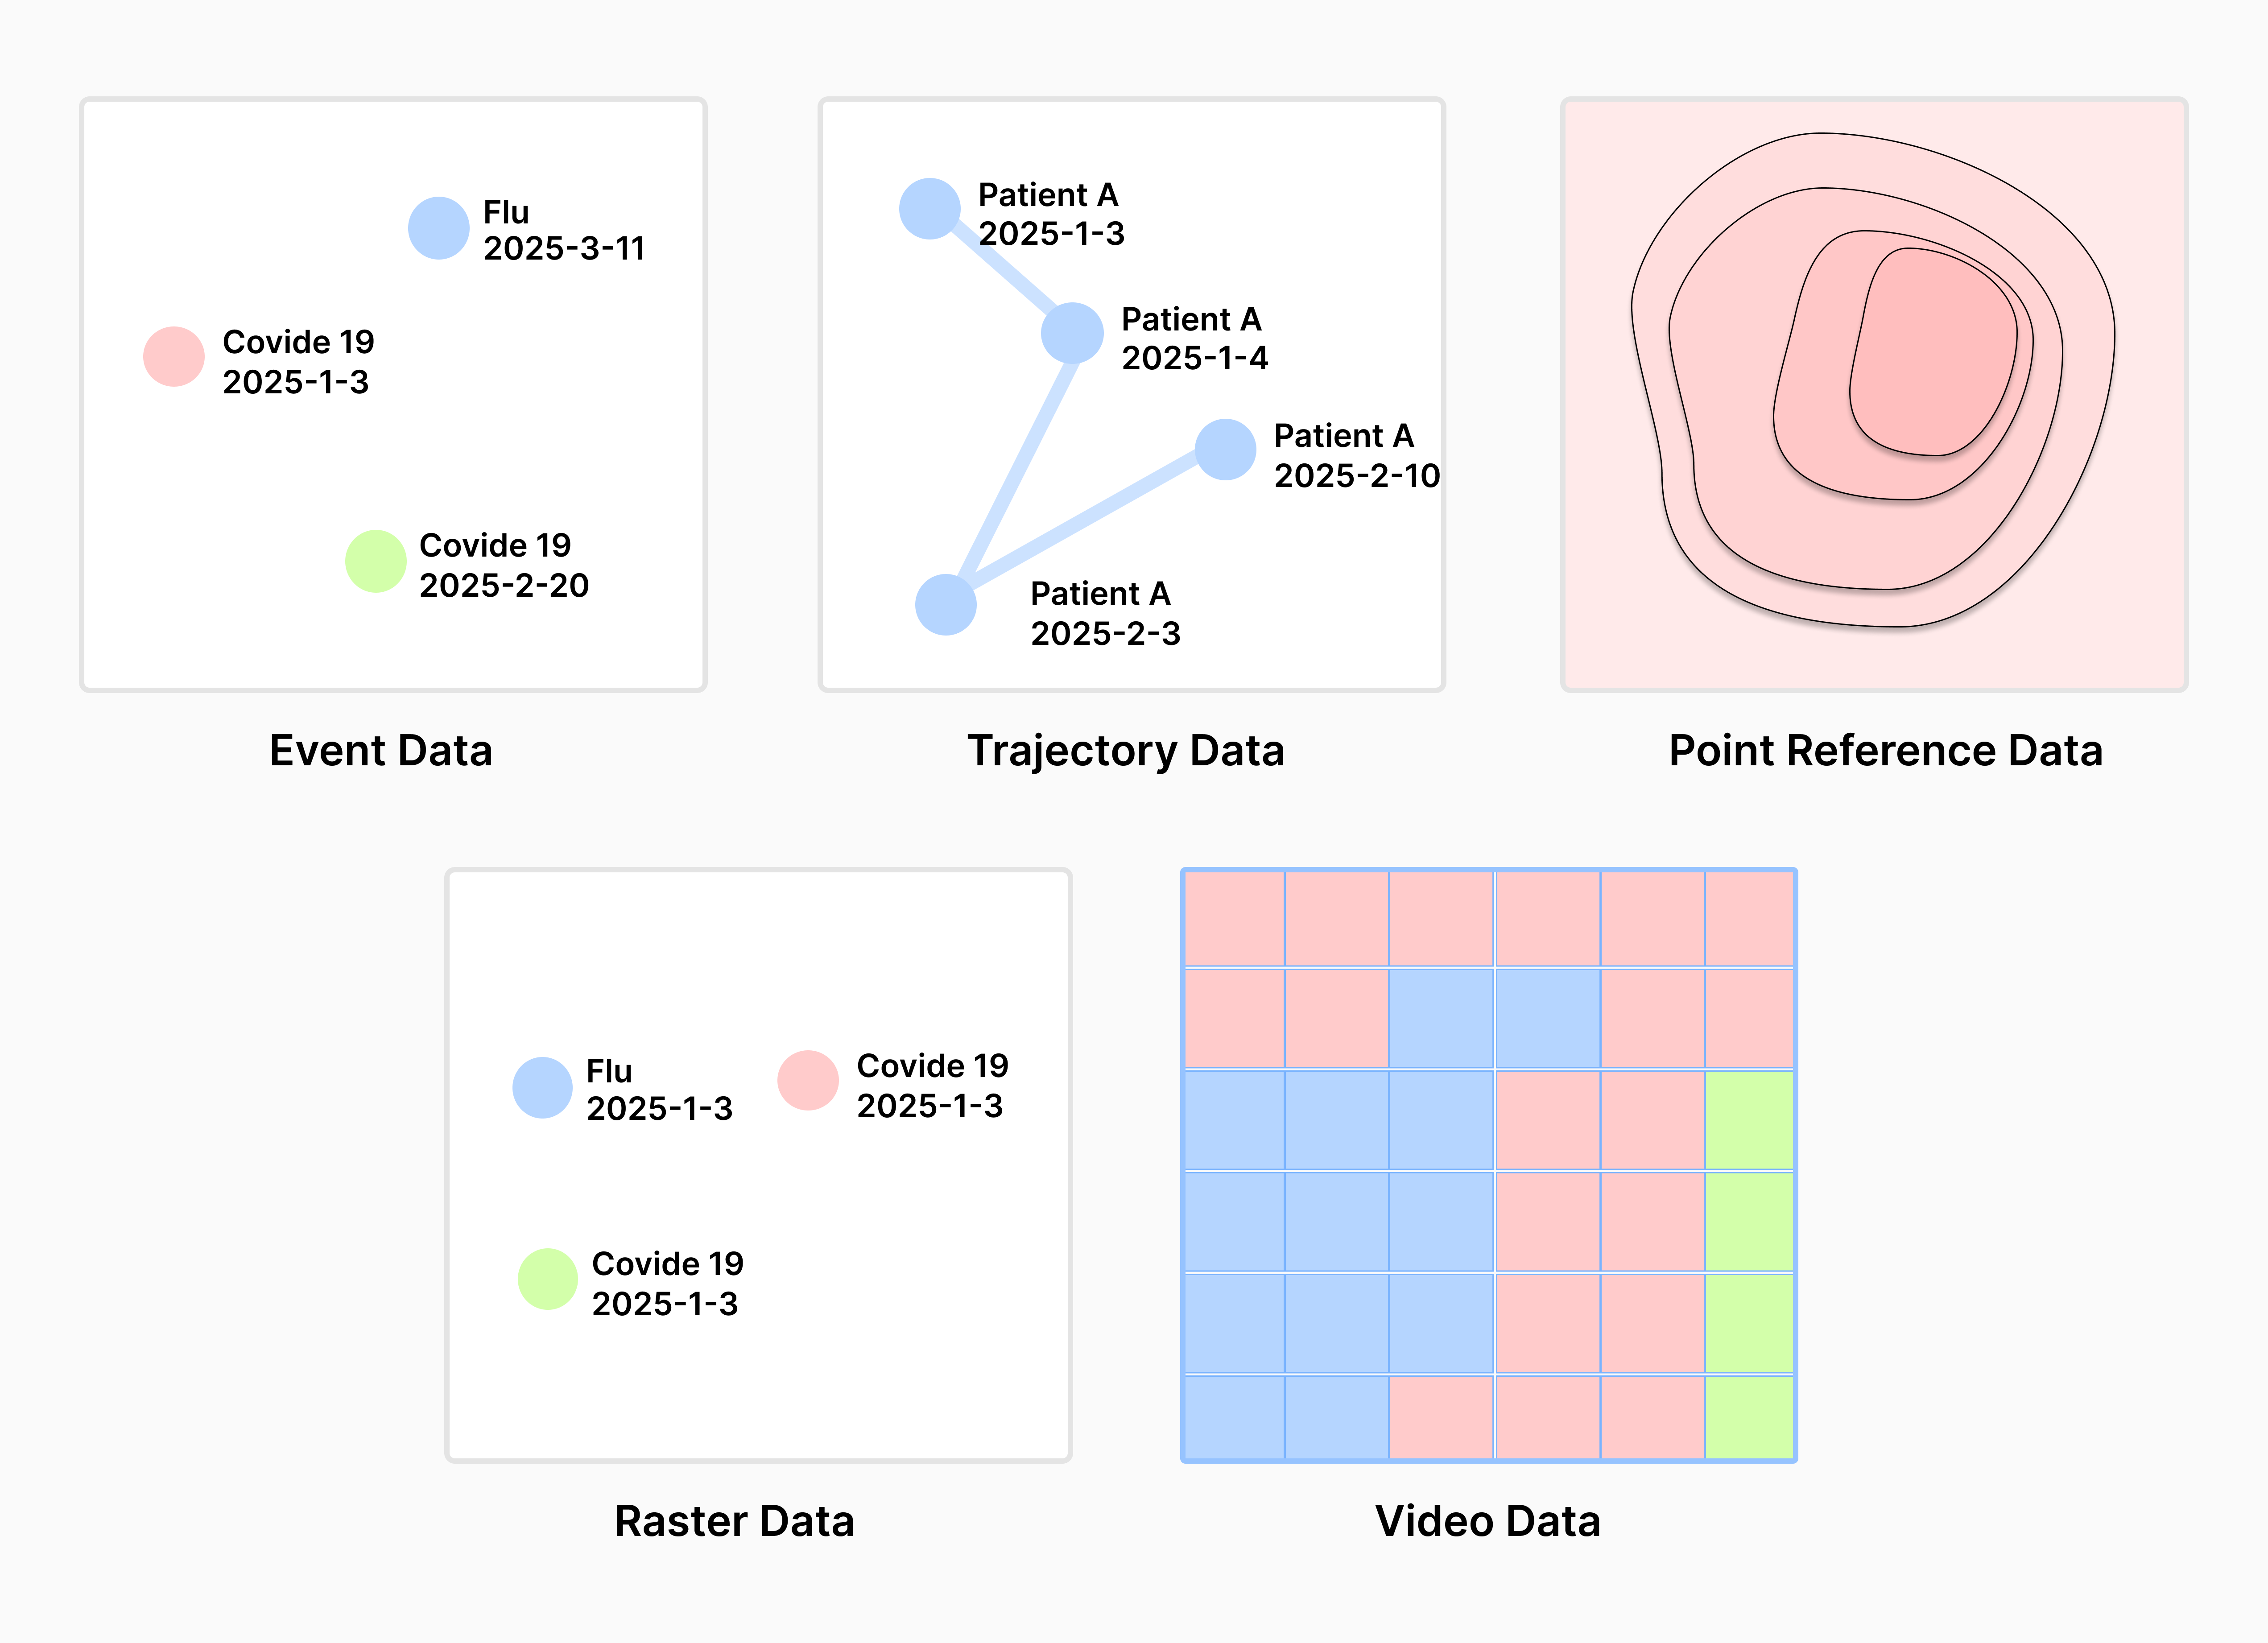
\includegraphics[width=\linewidth]{Fivecategories.png}
    \caption{The five categories of spatiotemporal data in digital health---event, trajectory, point reference, raster, and video data---each shown with a representative clinical example (e.g., outbreak reports, wearable mobility traces, vital-sign fields, hospital monitoring grids, and surgical video).}
    \Description{An illustration of the five categories of spatiotemporal data in digital health: event data, trajectory data, point-reference data, raster data, and video data, each paired with a representative clinical example.}
    \label{fig:Five Spatio temporal Data Categories}
\end{figure}

\textbf{Event data} consists of discrete single-point records in both time and space, typically 
structured as (location, time, event type). In digital health, representative examples include 
newly confirmed infectious disease cases, sudden surges in emergency visits, or outbreak reports 
for diseases such as influenza or COVID-19. Such data are commonly used for risk prediction, 
anomaly detection, and transmission chain analysis.

\textbf{Trajectory data} describes the continuous path of one or multiple entities over time, 
represented as an ordered series of (location, time) observations. In digital health, it arises 
from wearable devices recording personal mobility, ambulance routing, or mobile screening unit 
paths. These data support tasks such as path prediction, travel time estimation, and 
epidemiological analysis of how population movement shapes disease spread.

\textbf{Point reference data} takes the form (location, time, measurement), capturing sampled 
values of a target field --- such as air quality, heart rate, or blood pressure --- at specific 
locations. Rather than tracking entity movement, it focuses on precise measurements of 
environmental or physiological metrics, supporting field interpolation, anomaly detection, and 
multisensor fusion tasks.

\textbf{Raster data} consists of observations sampled at fixed spatial locations over regular 
time intervals, forming a structured matrix or tensor indexed by both space and time. Common 
digital health examples include daily outpatient volumes across hospital departments, fixed air 
quality monitoring stations, and fMRI brain imaging time series. Typical downstream tasks include 
spatiotemporal prediction, anomaly detection, and clinical segmentation.

\textbf{Video data} is composed of sequential image frames with high spatial and temporal 
resolution, capturing dynamic visual changes over time. In digital health, it appears primarily 
in surgical videos, ultrasound imaging, and endoscopic recordings, and is used for tasks such as 
lesion tracking, object detection, and action recognition in clinical and monitoring settings.

Beyond these five primitive types, much spatiotemporal health data also carries an explicit relational structure, in which individual measurements are linked by node--edge relationships, as in traffic and road networks, brain functional-connectivity graphs, or hospital and regional referral networks. Such graph-structured data is not a sixth, independent category; rather, it is a relational organization layered on top of the categories above --- most often on point reference and raster data --- in which fixed measurement sites, sensors, or regions become graph nodes and their spatial adjacency, topological connectivity, or functional correlations become edges. Modeling these data therefore reuses the same primitives while adding an explicit graph over them, and is handled by spatiotemporal graph neural networks (STGNN), discussed in Section~\ref{sec:history} and Section~\ref{sec:models}.

While all five types appear in digital health research, our primary interest throughout this
survey is in how patient covariates --- behavior, exposure, and physiology --- vary jointly 
across space and time. Trajectory data is therefore the most central form discussed, though the 
modeling principles introduced here generalize across these categories.

Public datasets further illustrate why trajectory centric spatiotemporal data is increasingly feasible in digital health research. The StudentLife study, for example, uses smartphone sensing to capture day to day and week to week behavioral patterns and links them to stress, sleep, sociability, and mental health related outcomes over time and across contexts~\cite{wang2014studentlife}. In addition, harmonized multi site nutrition and biomarker efforts are increasingly incorporating time indexed measurements and site level metadata, enabling analyses that connect dietary and physiological variation to context. As one example, the NIH funded iPAT project explicitly targets harmonized multi study dietary pattern analysis for chronic disease related research\cite{Fang2021iPAT}. Together, these resources suggest that the relationship between covariates and outcomes can be examined at a spatiotemporal level rather than only as static summaries.

Downstream tasks built on trajectory data in digital health can be grouped into several recurring goals. First, spatiotemporal feature aggregation aims to summarize how covariates evolve across time and context, for example by extracting multi scale temporal patterns and context sensitive exposures that are not visible from a single visit. Second, prediction tasks use spatiotemporal covariates to forecast future states, which may include predicting the next location or activity context, predicting future covariate values at a given time point and context, or directly predicting clinical outcomes and risks by modeling how covariates move along time and space. Third, spatiotemporal representations can support intervention oriented reasoning, where the goal is not only to predict what happens next, but to identify when and where interventions are most likely to reduce risk, for instance by linking mobility and context to lifestyle patterns such as diet and then suggesting context aware behavior adjustments. These task types are consistent with trajectory mining and mobility modeling literature, which emphasizes forecasting, representation learning, and decision support built on movement sequences.

Methodologically, three common strategies are widely used to process trajectory data. 
The first strategy is sequential modeling, which orders observations chronologically and applies sequence models to capture short-term and long-term temporal dependencies. Classic choices include recurrent models and gated variants, sequence-to-sequence architectures, and attention-based Transformers. This family is common in mobility prediction and trajectory forecasting, including models that handle sparse, long trajectories using attention mechanisms. These approaches are further discussed in Section~\ref{sec:history} and Section~\ref{sec:models}, particularly in the context of RNN-based and Transformer-based spatiotemporal models.The second strategy is spatial mapping, where trajectories are discretized into spatial units such as grids or mapped onto structured spatial supports such as road networks, after which convolutional models or spatial learning modules emphasize local proximity and spatial regularities. 
Related modeling techniques are introduced in Section~\ref{sec:history} and further elaborated in Section~\ref{sec:models}, including CNN-based and grid-based spatiotemporal representations. The third strategy is hybrid modeling, which combines temporal sequence learning with graph-based structure, for example by defining nodes and edges from road networks or interaction graphs and then coupling graph neural networks with temporal encoders. Such designs can enforce topological constraints and improve robustness under sparse sampling, which is common in real-world trajectories. 
These hybrid approaches are extensively discussed in Section~\ref{sec:models} and Section~\ref{sec:categorization}, particularly in the form of spatiotemporal graph neural networks (STGNN) and integrated architectures.

\subsection{Challenges of Sparsity, Irregularity, and Multi-scale Structure in Spatiotemporal Health Data}
While the previous sections illustrate why spatiotemporal models are theoretically well suited for digital health applications, practical data challenges substantially complicate their deployment. In ideal settings, spatiotemporal models benefit from dense and continuous observations, enabling accurate representation learning and strong predictive performance. In reality, however, health related spatiotemporal data are almost always characterized by sparsity and irregular sampling, which fundamentally constrain model design, training, and evaluation.

Temporal sparsity is a common and unavoidable property of medical and behavioral data. Clinical follow up periods often span many months or years, yet observations are recorded intermittently rather than continuously. Not every patient provides complete information at every time point, and missingness may arise from participant non-compliance, privacy concerns, or operational limits in data collection. As a result, sparsity should be viewed not as an exception but as a defining characteristic of real world digital health datasets, as has been noted in studies of longitudinal electronic health records and mobile sensing where data patterns are irregular and incomplete over time (e.g., irregular EHR time series and self-reports)~\cite{che2018grud}.

Beyond missing observations, temporal irregularity further complicates spatiotemporal modeling. Different hospitals and research institutions adopt distinct follow up schedules and data collection protocols, and when data from multiple sources are combined, the resulting time series frequently exhibit highly uneven intervals. Such irregular sampling violates the assumptions of many standard temporal models and may distort learned dynamics without explicit modeling of time intervals and relative sampling rates~\cite{shukla2021irregular}.

Challenges in the spatial dimension are closely related but manifest in different forms. Health related spatial data typically exist at multiple levels of granularity. At a coarse spatial granularity, location information is often recorded only as long term residential or regional attributes, such as home address or census level location, which may remain unchanged over extended periods. While this form of spatial information is more consistently available in large cohort and harmonized datasets, it is inherently sparse with respect to spatial transitions and may fail to capture environmental shifts and contextual exposures that influence disease progression. The importance of incorporating environmental and behavioral context into health research has been highlighted in studies that combine mobile sensing data with GPS and accelerometry to better understand behavioral drivers of chronic disease risk.

At a finer spatial granularity, data may reflect individuals’ short range, high frequency movements in daily life, such as visits to workplaces, food environments, or social venues. These fine grained mobility patterns are increasingly observable through wearable sensors and mobile devices, enabling environmental exposure estimation and context aware analyses that were previously infeasible. However, such data are often noisy, incomplete, and unevenly available across individuals and time periods. Effectively extracting health relevant signals from detailed but irregular spatial traces remains challenging, particularly when distinguishing meaningful contextual exposures from incidental movement.

Importantly, fine and coarse spatial representations are not independent. Short term mobility patterns are embedded within long term residential contexts, and spatial covariates across scales may exhibit strong correlations and hierarchical dependency. Modeling these cross scale relationships introduces additional challenges, including redundancy, confounding effects, and scale mismatch. Similar multi-scale structure also exists in the temporal dimension, where short term dynamics and long term trends coexist and interact, further complicated by irregular sampling across data sources. Addressing these intertwined multi scale challenges is crucial for robust spatiotemporal modeling in digital health.

Together, temporal sparsity, irregular sampling, heterogeneous spatial granularity, and cross scale dependency constitute central challenges for spatiotemporal modeling in digital health. Addressing these issues requires models that are robust to missing and irregular observations while effectively integrating information across multiple spatial and temporal scales.

\section{History of Deep Learning–Based Spatiotemporal Modeling Methods in Digital Health}
\label{sec:history}
After understanding the applicability of Spatiotemporal data in digital health, as well as the corresponding data processing methods and applications, let us first review the historical development of Spatiotemporal models and explore the research surrounding different Spatiotemporal forecasting categories. We will then provide a detailed introduction to the mainstream Spatiotemporal models before moving on to their applications in digital health.

\subsection{The Historical Development of Spatiotemporal Models in Digital Health}
Historically, the exploration of deep learning for ST tasks commenced with simpler feed-forward networks such as Multilayer Perceptrons (MLPs). Early applications (pre-2015) adapted MLPs primarily for time-series prediction (e.g., forecasting disease incidence or patient visits~\cite{miotto2018deeplearning}), albeit with limited capacity to handle complex spatial relationships. Subsequently, RNNs and LSTMs gained prominence by extending the modeling scope to longer sequences and more nuanced temporal dynamics. By incorporating spatial structures into LSTM cells (e.g., ST-LSTM), these architectures could capture both spatial and temporal correlations, making them valuable in tasks like epidemic forecasting and wearable device data analytics.

Between 2015 and 2020, Spatiotemporal graph neural networks (STGNN) and attention-based mechanisms (e.g., Transformers) emerged. STGNNs introduced graph convolutional layers to model non-Euclidean spatial relationships, broadening potential use cases from city-wide traffic flow prediction to hospital network analyses. Meanwhile, Transformers and self-attention-based architectures such as ST-Transformer offered greater flexibility in capturing long-range dependencies. These breakthroughs facilitated multi-modal data fusion by integrating imaging, EHR, wearable device signals, and environmental data into a single predictive pipeline~\cite{caroprese2018deepehr}.

Since 2020, ST deep learning approaches have increasingly combined Transformers, self-supervised learning, and multi-modal fusion to capture fine-grained Spatiotemporal dependencies. Exemplars include TimeSformer and ST-Transformer variants for modeling large-scale medical imaging sequences and climate-health interactions~\cite{liu2024temporallearning}. As model complexity and data modalities continue to grow, federated learning has also emerged as a critical privacy-preserving framework, enabling model training across distributed medical datasets without compromising patient confidentiality.

In parallel, recent work in leading statistics journals has strengthened the statistical foundations that are useful for digital-health ST modeling, even when the final predictive model is deep neural. Representative examples include physics-informed convection--diffusion models, Lagrangian cross-covariance functions, score-driven ST models, semiparametric autoregressive models for irregular nonstationary locations, dynamic-deformation covariance models, graphical models for nonstationary time series, spatiotemporal varying-coefficient disease mapping, spatial SIR emulators, and statistical deep-learning syntheses for spatial and spatiotemporal data~\cite{liu2022convectionDiffusion,salvana2023lagrangian,gasperoni2023scoreDriven,lu2024dyfast,castroMorales2025dynamicDeformation,basu2023graphicalNonstationary,wang2024respiratoryDiseaseMapping,trostle2024spatialSIR,wikle2023statisticalDeepLearning}. These papers complement DNN-based approaches by providing interpretable covariance structures, physical constraints, uncertainty quantification, and principled baselines for evaluating neural spatiotemporal models.

We have reviewed the models mentioned above and will begin by briefly introducing several common foundational neural network architectures—CNN, GNN, RNN, and Transformer. Building on these, we then present the following mainstream Spatiotemporal models:
	1.	CNN-RNN Hybrid Models: These leverage Convolutional Neural Networks (CNN) to extract spatial features and employ Recurrent Neural Networks (RNN) to capture temporal dependencies in time series data.
	2.	Spatiotemporal Graph Neural Networks (STGNN): By conducting Spatiotemporal modeling on graph structures, these models use Graph Neural Networks (GNN) to represent spatial relationships among nodes, combined with time-series models to capture temporal dependencies.
	3. Transformer Models for ST Data: Relying on attention mechanisms, these models efficiently capture dependencies over long temporal and spatial ranges and perform well in spatiotemporal forecasting tasks.
    4. 3D CNN and Hybrid Networks: Designed for high dimensional spatiotemporal data such as video, these approaches combine 3D convolution with other modules or networks to better capture spatiotemporal features.

Within each of these architectures, we also discuss their applications in the domain of digital health.

\begin{figure}
    \centering
    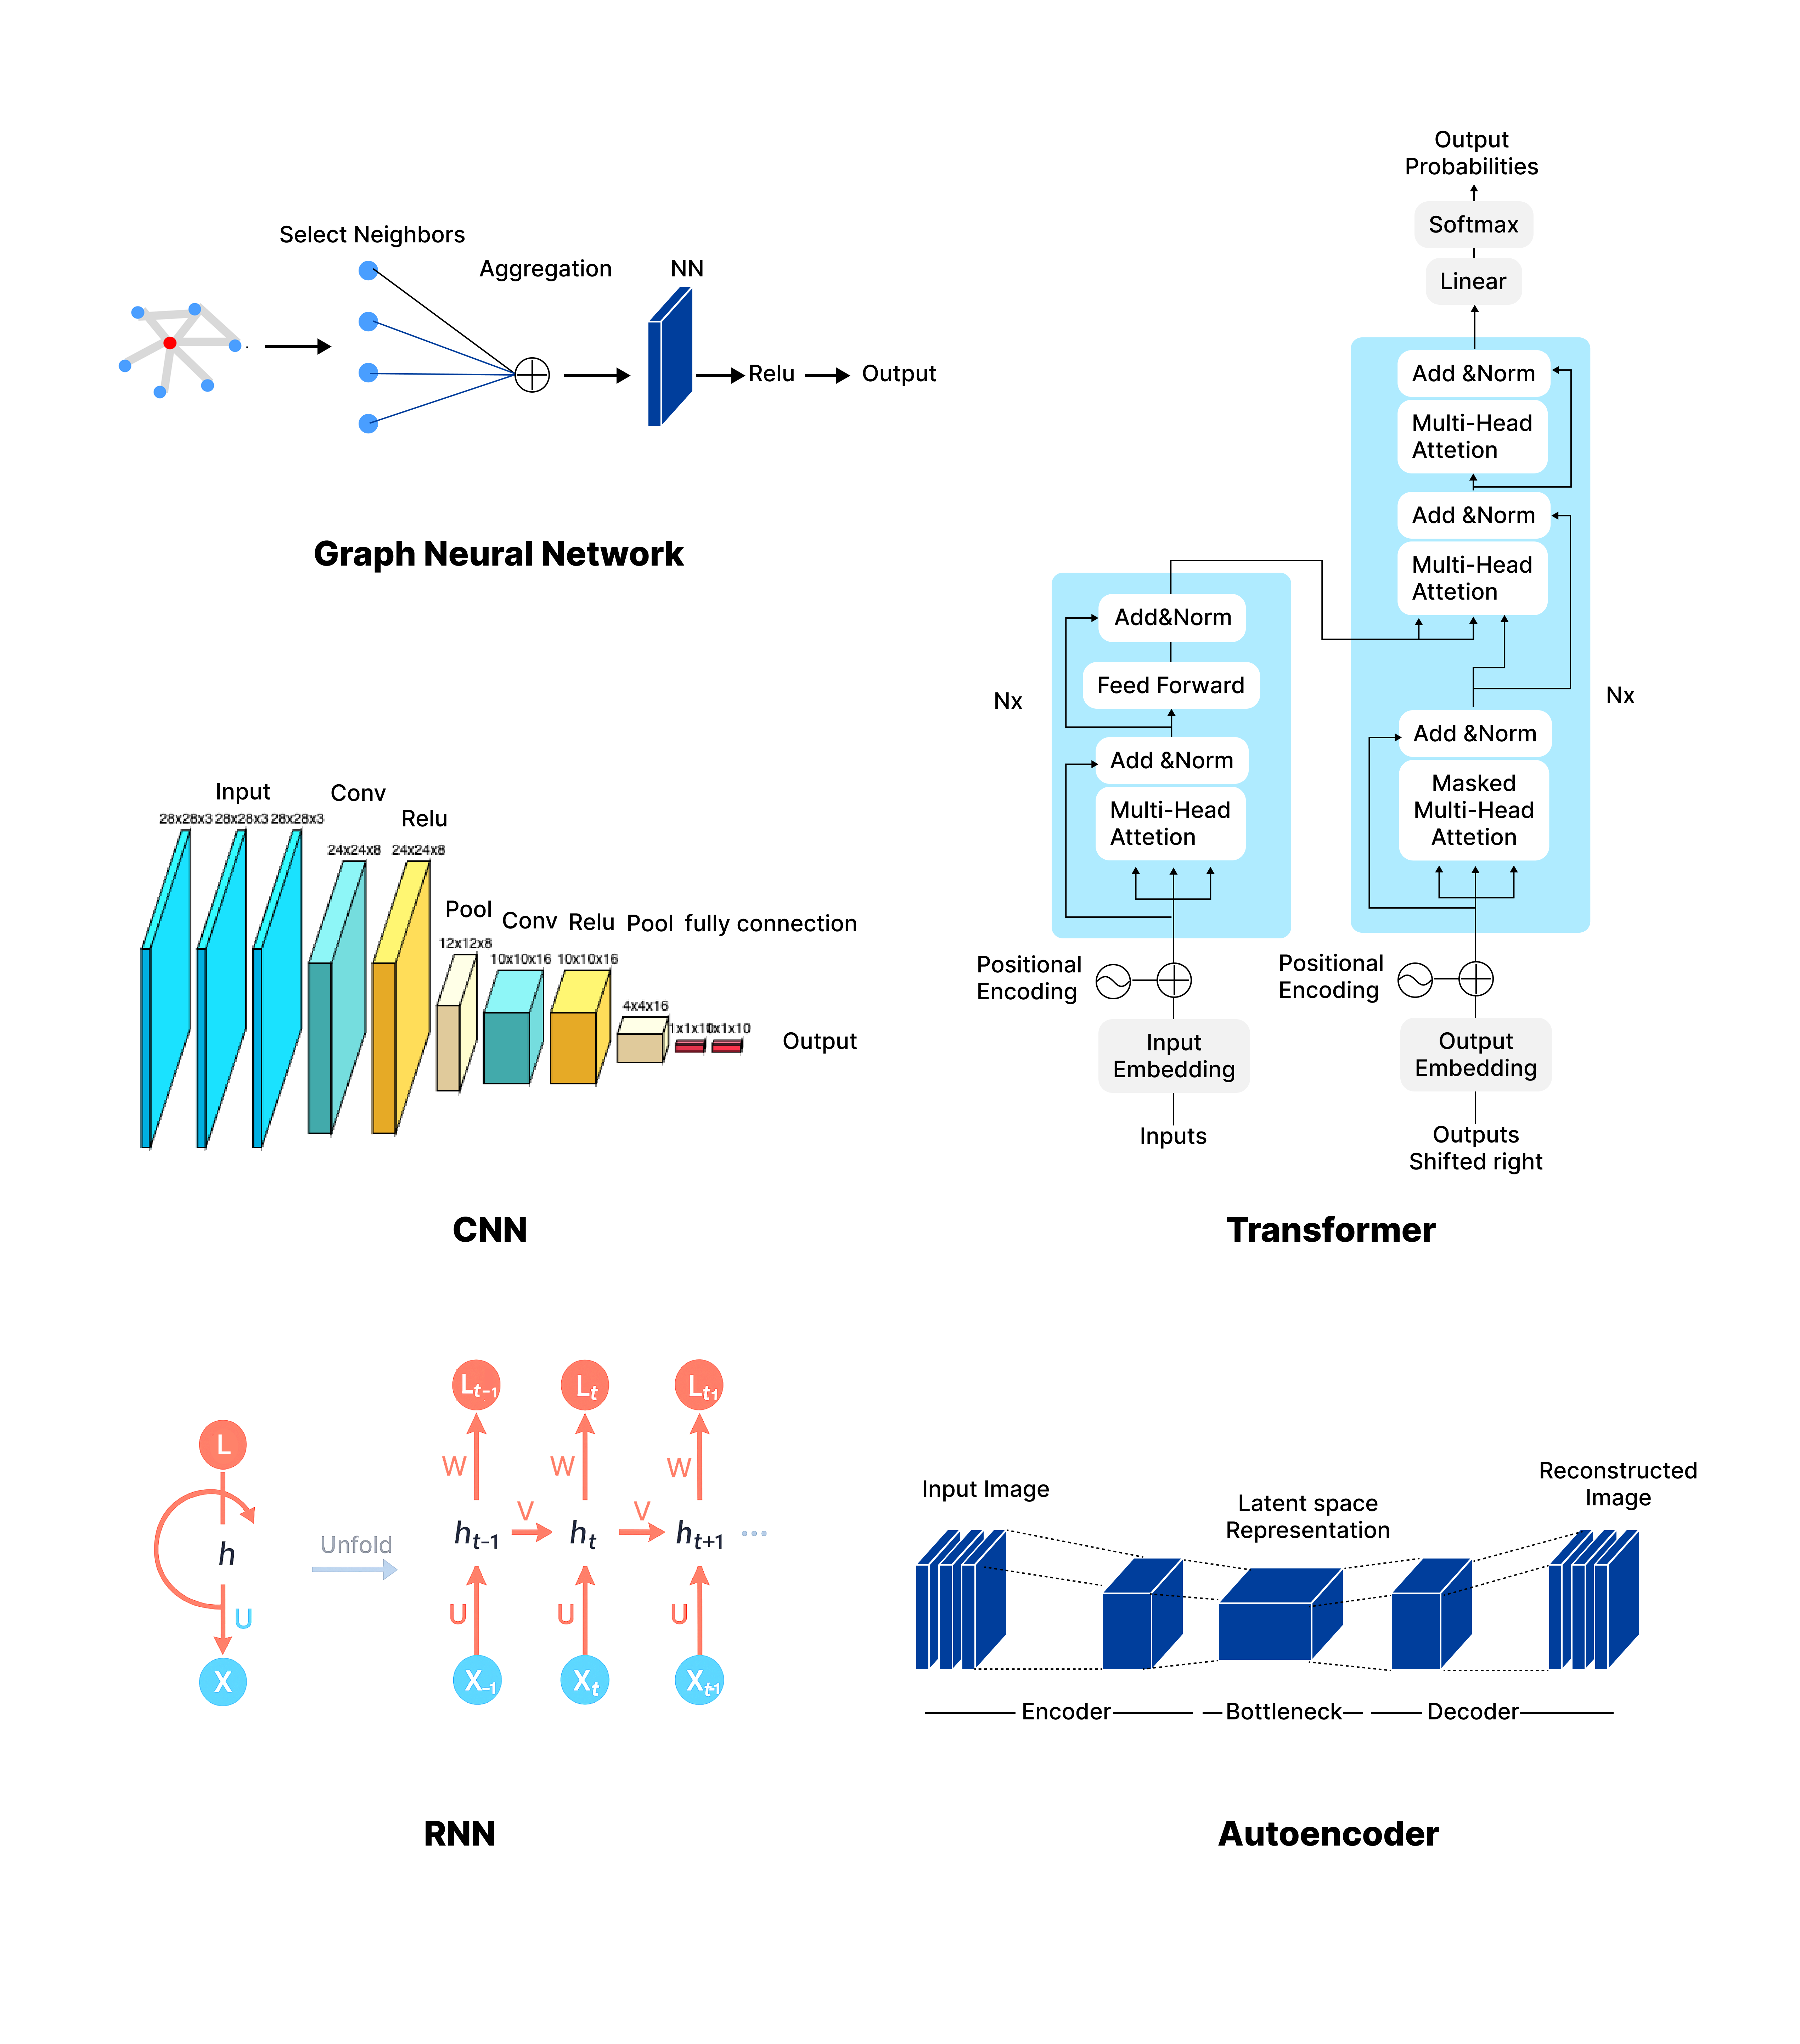
\includegraphics[width=1\linewidth]{Frame 34.png}
    \caption{A general spatiotemporal modeling pipeline for digital health: foundational deep learning architectures (CNN, GNN, RNN, Transformer, and autoencoders) transform raw spatiotemporal health data into clinical predictions, forming the basis for the specialized model families surveyed in Sections~\ref{sec:history}--\ref{sec:categorization}. Figure~\ref{fig:foundation_arch} details the internal structure of several of these architectures.}
    \Description{A schematic of a general spatiotemporal modeling pipeline for digital health, showing how raw spatiotemporal health data are encoded by foundational deep learning architectures (CNN, GNN, RNN, Transformer, and autoencoders) and mapped to clinical prediction tasks.}
    \label{fig:GeneralModel}
\end{figure}

\begin{figure}
    \centering
    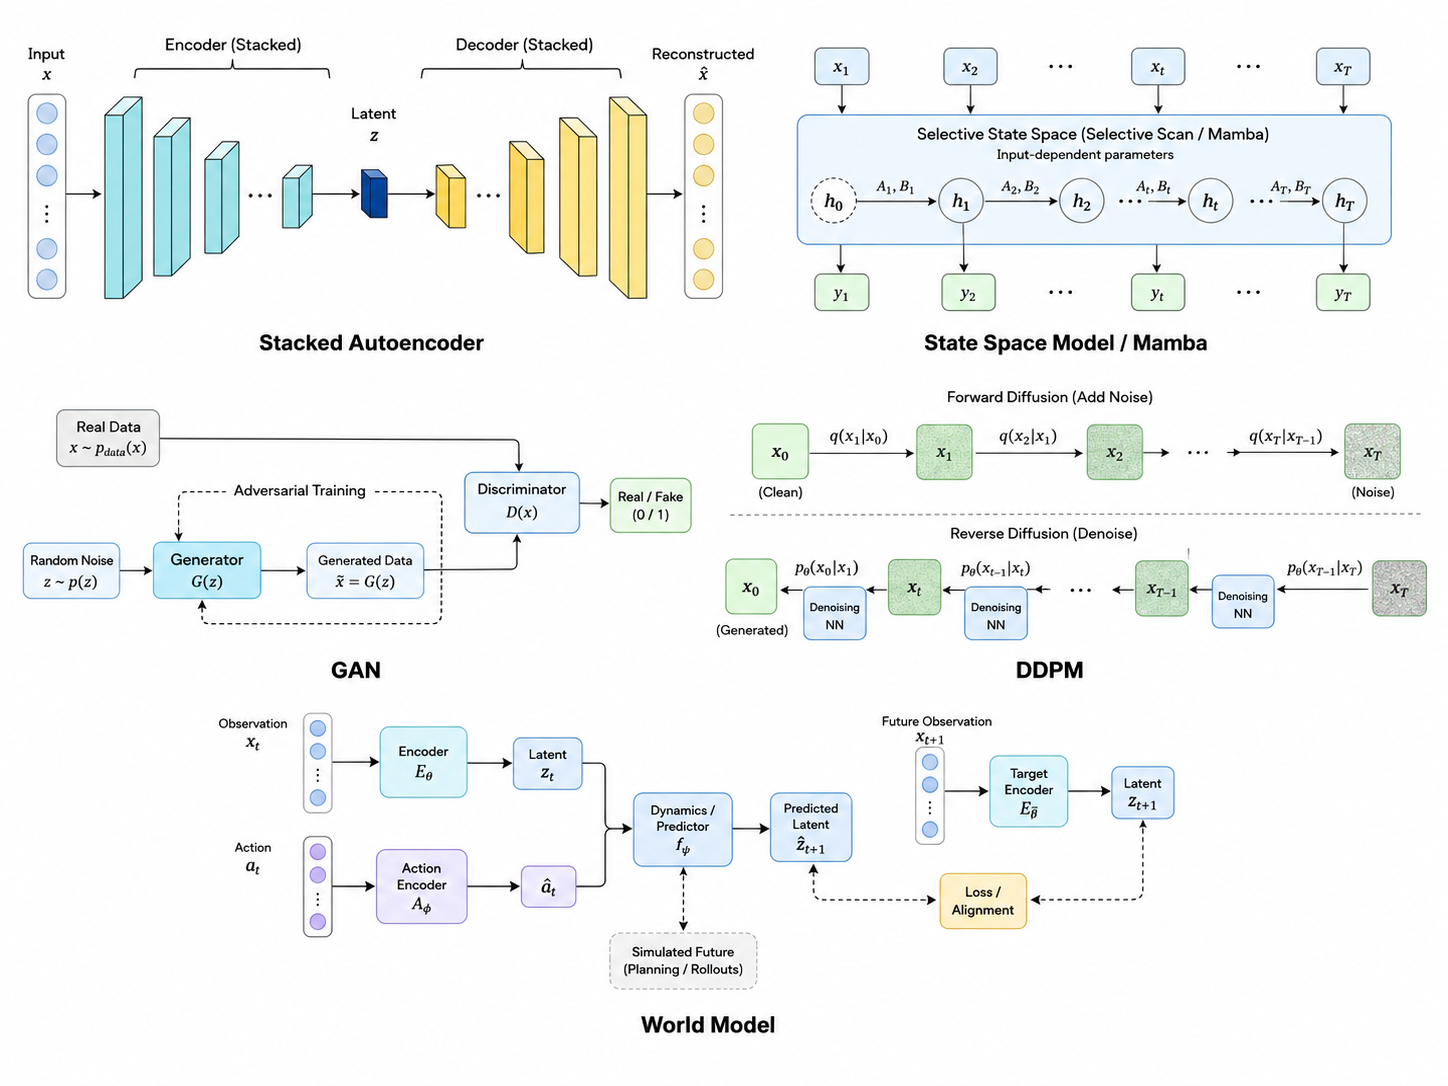
\includegraphics[width=\linewidth]{arch2.png}
    \caption{Internal structure of five foundational deep learning architectures, complementing the pipeline overview in Figure~\ref{fig:GeneralModel}. The stacked autoencoder compresses an input into a latent code and reconstructs it through stacked encoder and decoder layers; the state space model (Mamba) propagates an input dependent hidden state across time through a selective scan; the generative adversarial network (GAN) trains a generator against a discriminator that separates real from synthetic samples; the denoising diffusion probabilistic model (DDPM) corrupts data with noise in a forward process and learns to reverse it to generate clean samples; and the world model encodes an observation and an action into a latent state, predicts the next latent state, and aligns it with a target encoding of the future observation to support simulation and planning.}
    \Description{Five panels showing the architectures of a stacked autoencoder, a state space model (Mamba), a generative adversarial network, a denoising diffusion probabilistic model, and a world model, each drawn as a block diagram with its inputs, latent states, and outputs.}
    \label{fig:foundation_arch}
\end{figure}

\subsection{Foundational Deep Learning Architectures}
Building on the core concepts of deep learning introduced earlier, this section provides an overview of general deep-learning-based architectures that form the foundation for many advanced Spatiotemporal models. By understanding how fundamental structures such as Graph Neural Networks (GNNs) \cite{scarselli2009gnn}, Recurrent Neural Networks (RNN) \cite{rumelhart1986rnn}, Transformers \cite{vaswani2017attention}, AutoEncoders (AEs) \cite{hinton2006reducing}, Stacked AutoEncoders (SAEs) \cite{masci2011stacked}, State-Space Models including Mamba \cite{gu2023mamba}, Generative Adversarial Networks (GANs) \cite{goodfellow2014gan}, Denoising Diffusion Probabilistic Models (DDPMs) \cite{ho2020ddpm}, and World Models \cite{maes2026leworldmodel} operate, as shown in Figure~\ref{fig:GeneralModel} and Figure~\ref{fig:foundation_arch}, we can better appreciate their extensions and adaptations for complex tasks. The following subsections delve into these key components, setting the stage for specialized Spatiotemporal techniques.

\paragraph{Graph Neural Networks (GNNs)}: Many real-world applications involve data structured as graphs, such as social networks, molecular structures, transportation systems, and recommendation engines. Traditional deep learning methods, including CNNs \cite{lecun1998cnn} and RNNs, excel in handling tabular, sequential, and image data but struggle with non-Euclidean structures like graphs. Graph Neural Networks (GNNs) \cite{scarselli2009gnn} extend neural network capabilities to directly process graph-structured data, capturing both local and global structural relationships.

A graph is typically represented as $G = (V, E)$, where:
- $$V = \{v_1, v_2, ..., v_N\}$$ denotes the set of nodes.
- $E \subseteq V \times V$ represents the set of edges (connections between nodes).
- Each node $v_i$ may have a feature vector $h_i$ representing its attributes.

The goal of GNNs is to learn node embeddings that encapsulate both graph topology and node-specific properties.

GNNs operate using a message passing and neighborhood aggregation framework, where each node updates its feature representation by aggregating information from its neighbors.

At layer $l$, the message from neighboring nodes is aggregated as:

\begin{equation}
m_i^{(l)} = \sum_{j \in N(i)} f(h_j^{(l-1)}, h_i^{(l-1)}, e_{ij})
\end{equation}

where $h_i^{(l-1)}$ represents the previous layer’s node features, $e_{ij}$ is the edge feature (if available), and $f(\cdot)$ defines the aggregation function, which can be a weighted sum or an MLP.

After aggregation, each node updates its representation via a non-linear transformation:

\begin{equation}
h_i^{(l)} = \sigma(W m_i^{(l)} + b)
\end{equation}

where $W$ and $b$ are trainable parameters, and $\sigma$ is a non-linear activation function such as Rectified Linear Unit (ReLU).

Different GNN architectures adopt distinct aggregation and update mechanisms, including:
Graph Convolutional Networks (GCN):Uses spectral graph convolutions for information propagation\cite{kipf2017gcn}.
Graph Attention Networks (GAT): Introduces attention mechanisms to weigh contributions from different neighbors \cite{velickovic2018gat}.
Graph Isomorphism Networks (GIN): Enhances expressiveness by leveraging MLP-based feature transformations \cite{xu2019gin}.

By leveraging these models, GNNs provide a powerful framework for learning representations from graph-structured data, enabling applications across multiple domains.

\paragraph{Recurrent Neural Networks (RNN) and Their Variants}: Before the widespread adoption of Transformer models, recurrent neural networks (RNNs)\cite{rumelhart1986rnn} and their variants were widely used for time series modeling. RNNs use recurrent connections, allowing the hidden state at time step $t$ to depend on the previous hidden state, capturing temporal dependencies. Given an input sequence $X = (x_1, x_2, ..., x_T)$, the hidden state and output are computed as:

\begin{equation}
h_t = f(W_h h_{t-1} + W_x x_t + b_h), \quad y_t = g(W_y h_t + b_y)
\end{equation}

where $W_h, W_x, W_y$ are weight matrices, $b_h, b_y$ are biases, $f(\cdot)$ is a nonlinear activation function (e.g., tanh or ReLU), and $g(\cdot)$ is typically softmax for classification. However, standard RNNs suffer from vanishing and exploding gradients, making long-term dependency learning difficult.

Long Short-Term Memory (LSTM)\cite{rnn_lstm} networks address this issue with gating mechanisms: the forget gate, input gate, and output gate, along with a cell state to store long-term information. The LSTM updates are as follows:

\begin{equation}
f_t = \sigma(W_f [h_{t-1}, x_t] + b_f), \quad i_t = \sigma(W_i [h_{t-1}, x_t] + b_i)
\end{equation}
\begin{equation}
\tilde{C}_t = \tanh(W_C [h_{t-1}, x_t] + b_C), \quad C_t = f_t \odot C_{t-1} + i_t \odot \tilde{C}_t
\end{equation}
\begin{equation}
o_t = \sigma(W_o [h_{t-1}, x_t] + b_o), \quad h_t = o_t \odot \tanh(C_t)
\end{equation}

where $\sigma(\cdot)$ is the sigmoid function, $\tanh(\cdot)$ is the hyperbolic tangent function, and $\odot$ denotes element-wise multiplication. LSTM’s gating mechanism allows effective long-term information retention while filtering out irrelevant details. 

\paragraph{Transformer Model}: The Transformer model \cite{vaswani2017attention} consists of an encoder and a decoder, both composed of multiple stacked layers. Each layer includes a multi-head self-attention mechanism (MHSA), a feedforward neural network (FFN), and residual connections. The architecture follows the structure:

\begin{equation*}
\text{Input Sequence} \xrightarrow{\text{Embedding Layer}} \text{Encoder} \rightarrow \text{Decoder} \xrightarrow{\text{Output Layer}} \text{Prediction}
\end{equation*}

The encoder is formed by $N$ identical layers, each containing multi-head self-attention, FFN, layer normalization, and residual connections. The input sequence $X \in \mathbb{R}^{T \times d}$ is embedded and passed to the encoder, where self-attention representations are computed.

The decoder follows a similar structure but includes masked multi-head self-attention to prevent seeing future tokens during training (causal masking). Additionally, an encoder-decoder attention mechanism allows the decoder to incorporate encoder outputs. The final output is generated via a Softmax layer.

At the core of Transformer is the self-attention mechanism, which determines the importance of each element relative to others. Given an input sequence $X$, the self-attention weights are computed as follows:

\begin{equation}
Q = X W_Q, \quad K = X W_K, \quad V = X W_V
\end{equation}

where $Q, K, V$ are the query, key, and value matrices, and $W_Q, W_K, W_V$ are learnable weights. The attention scores are calculated using:

\begin{equation}
\text{Attention}(Q, K, V) = \text{softmax} \left(\frac{Q K^T}{\sqrt{d_k}} \right) V
\end{equation}

where $d_k$ is the key dimension, and $\frac{1}{\sqrt{d_k}}$ is a scaling factor to prevent large gradients. This mechanism enables the model to capture long-range dependencies efficiently.

\paragraph{AutoEncoder (AE) and Stacked AutoEncoder (SAE)}: AutoEncoder (AE) is an unsupervised learning model consisting of an encoder and a decoder. The encoder maps the input data $\mathbf{x} \in \mathbb{R}^{n}$ to a lower-dimensional latent representation $\mathbf{h}$, while the decoder reconstructs the original input from this latent representation. The encoding and decoding processes are defined as follows:
\begin{equation}
\mathbf{h} = f(\mathbf{x}) = \sigma(\mathbf{W}_e \mathbf{x} + \mathbf{b}_e),
\end{equation}
\begin{equation}
\hat{\mathbf{x}} = g(\mathbf{h}) = \sigma'(\mathbf{W}_d \mathbf{h} + \mathbf{b}_d),
\end{equation}
where $\sigma(\cdot)$ and $\sigma'(\cdot)$ are activation functions, and $\mathbf{W}_e, \mathbf{b}_e$, $\mathbf{W}_d, \mathbf{b}_d$ are the weights and biases of the encoder and decoder, respectively. The objective function minimizes the reconstruction error, often using mean squared error (MSE):
\begin{equation}
L(\mathbf{x}, \hat{\mathbf{x}}) = \| \mathbf{x} - \hat{\mathbf{x}} \|^2.
\end{equation}
Hinton and Salakhutdinov \cite{hinton2006reducing} introduced deep AEs for dimensionality reduction, laying the foundation for subsequent deep learning advancements.

In Spatiotemporal modeling, AEs are employed to capture local spatial and temporal patterns. They have been successfully applied in traffic flow prediction, environmental monitoring, and other applications where feature extraction is critical \cite{vincent2008extracting, bengio2009learning}.

Stacked AutoEncoder (SAE) extends AE by stacking multiple layers of AEs to form a deeper architecture. By pre-training each layer separately and then fine-tuning the entire model, SAE effectively extracts high-level abstract representations of complex Spatiotemporal data. The training process of SAE typically involves two stages: first, each AE layer is trained independently, and then all layers are fine-tuned together \cite{erhan2010why, ranzato2007unsupervised}. In DNN-based Spatiotemporal models, SAEs enhance multiscale feature extraction, providing a powerful representation capability \cite{masci2011stacked, vincent2010stacked}.

Furthermore, Variational AutoEncoders (VAE) \cite{kingma2013auto} introduced a probabilistic perspective to AEs, expanding their applications in Spatiotemporal data representation and generation. Understanding the challenges in training deep neural networks \cite{glorot2010understanding} also contributes to the effective application of SAEs in complex tasks. Combining these approaches, modern DNN-based Spatiotemporal models have demonstrated superior performance in traffic prediction, weather analysis, and video understanding \cite{zhang2017deep, yu2018spatio}.

\paragraph{State Space Models and Mamba}: State space models (SSMs) describe a sequence through a latent state that evolves linearly over time, offering an efficient alternative to attention for long-range temporal modeling. A continuous SSM maps an input $x(t)$ to an output $y(t)$ through a hidden state $h(t)$, and after discretization with step size $\Delta$ it reduces to a linear recurrence:
\begin{equation}
h_t = \bar{A} h_{t-1} + \bar{B} x_t, \quad y_t = C h_t,
\end{equation}
where $\bar{A}$ and $\bar{B}$ are the discretized state and input matrices and $C$ is the output matrix. Because this recurrence is linear, it can be unrolled as a global convolution, enabling efficient training over very long sequences---a property exploited by the Structured State Space (S4) family and its Spatiotemporal extensions \cite{smith2023convssm}. Mamba \cite{gu2023mamba} further makes the SSM parameters input dependent (a selective mechanism), allowing the model to emphasize relevant context while maintaining linear time complexity and constant memory usage during inference. In spatiotemporal digital health, these properties are attractive for modeling long, densely sampled physiological streams such as continuous glucose monitoring, ECG, and EEG, as well as long videos and longitudinal trajectories spanning multiple years, where the quadratic cost of standard attention becomes prohibitive.

\paragraph{Generative Adversarial Networks (GANs)}: Generative Adversarial Networks (GANs) \cite{goodfellow2014gan} learn to generate realistic data through a two-player game between a generator $G$, which maps a noise vector $z$ to a synthetic sample $G(z)$, and a discriminator $D$, which estimates the probability that a sample is real rather than generated. The two networks are trained jointly by optimizing the minimax objective:
\begin{equation}
\min_G \max_D \; \mathbb{E}_{x \sim p_{\text{data}}}[\log D(x)] + \mathbb{E}_{z \sim p_z}[\log (1 - D(G(z)))].
\end{equation}
At convergence, the generator reproduces the data distribution while the discriminator can no longer distinguish real from synthetic samples. In Spatiotemporal digital health, GANs are widely used to synthesize realistic medical images and physiological signals, to augment scarce or imbalanced cohorts, and to impute missing values in irregular time series; conditional and temporal GAN variants further enable the generation of Spatiotemporal sequences conditioned on patient context.

\paragraph{Denoising Diffusion Probabilistic Models (DDPMs)}: Denoising Diffusion Probabilistic Models (DDPMs) \cite{ho2020ddpm} are generative models that gradually corrupt data with Gaussian noise and then learn to reverse this process. The forward process adds noise over $T$ steps according to a variance schedule $\{\beta_t\}$:
\begin{equation}
q(x_t \mid x_{t-1}) = \mathcal{N}\!\left(x_t; \sqrt{1-\beta_t}\, x_{t-1}, \; \beta_t \mathbf{I}\right),
\end{equation}
and a neural network $\epsilon_\theta$ is trained to predict the added noise by minimizing the simplified objective:
\begin{equation}
L = \mathbb{E}_{x_0, \epsilon, t}\!\left[\, \left\| \epsilon - \epsilon_\theta(x_t, t) \right\|^2 \,\right].
\end{equation}
New samples are produced by iteratively denoising from pure noise. Compared with GANs, diffusion models offer more stable training and higher sample fidelity, and in Spatiotemporal digital health they are increasingly applied to high-fidelity generation and denoising of medical images and physiological signals, to imputation of missing or irregularly sampled measurements, and to data augmentation for downstream Spatiotemporal prediction.

\paragraph{World Models}: World models learn a compact internal model of how an environment evolves, so that future states can be predicted and candidate actions evaluated through simulation rather than direct trial. A common design encodes high-dimensional observations into a latent state and predicts its evolution in that latent space; recent Joint-Embedding Predictive Architectures (JEPA) train the predictor to match the latent representation of future observations \cite{maes2026leworldmodel}. Formally, an encoder $E_\theta$ maps an observation $x_t$ to a latent state, a predictor $P_\phi$ rolls the latent state forward under an action $a_t$, and the model is trained to align the prediction with the target-encoded future observation:
\begin{equation}
z_t = E_\theta(x_t), \quad \hat{z}_{t+1} = P_\phi(z_t, a_t), \quad L = \left\| \hat{z}_{t+1} - E_{\bar{\theta}}(x_{t+1}) \right\|^2,
\end{equation}
where $E_{\bar{\theta}}$ denotes a slowly updated target encoder. In spatiotemporal digital health, world models provide a principled basis for patient state simulation and counterfactual planning by predicting how a patient's trajectory would respond to alternative interventions before they are implemented, and they also underpin the digital twins based on world models discussed in Section~\ref{sec:DT}.


% \subsection{Spatiotemporal Model}
% While general DNN frameworks like Transformers and AEs excel at feature learning, many real world challenges involve both space and time dimensions. In this section, we shift our focus to Spatiotemporal models, which integrate spatial feature extraction with temporal sequence modeling. These models address tasks such as traffic prediction, meteorological forecasting, and video analysis by capturing interactions across both space and time. We will explore various architectures—from 3D CNN, CNN-RNN hybrids to graph-based and Transformer-based solutions that build upon the fundamentals described in the previous section.

% \paragraph{CNN-RNN Hybrid Model}The CNN-RNN hybrid model is one of the earliest deep learning architectures applied to ST modeling. This model extracts spatial features using Convolutional Neural Networks (CNN) and learns temporal dependencies using Recurrent Neural Networks (RNN), such as Long Short-Term Memory (LSTM) or Gated Recurrent Units (GRU). This approach has demonstrated effectiveness in tasks like weather forecasting and video analysis. For instance, Li et al.~\cite{li2025solar} proposed a hybrid deep learning framework for solar radiation forecasting, utilizing CNN for spatial feature extraction and LSTM for capturing temporal dependencies, significantly improving prediction accuracy. However, a major drawback of this model is its high computational complexity and the potential vanishing gradient problem when dealing with long-term dependencies.

% \paragraph{ST Graph Neural Networks (STGNN)} ST Graph Neural Networks (STGNN) \cite{shao2022longterm} have gained significant attention for modeling complex, non-Euclidean spatial data, such as traffic flow and power grid monitoring. STGNNs utilize Graph Neural Networks (GNN) to model spatial relationships between nodes while employing temporal models like LSTM or Transformer to learn temporal evolution patterns. For example, Wang et al.~\cite{wang2025rul} proposed a Graph Feature Attention Network (GFAN)-based method for predicting the remaining useful life of multi-sensor systems, effectively capturing ST dependencies between sensors. Although STGNNs perform well in many applications, they are computationally expensive and require significant resources for large-scale graph data processing.

% \paragraph{Transformer-based ST model} Transformer-based ST models have become a research hotspot in recent years. The self-attention mechanism in Transformer architectures allows them to capture long-range dependencies effectively, making them highly suitable for ST sequence modeling. Unlike traditional RNN-based models, Transformers handle long-term dependencies more efficiently. For example, Yu et al.~\cite{yu2025graph} introduced a method integrating dynamic Transformers with Graph Diffusion Learning (GDL) to improve anomaly detection in multivariate time series. Additionally, Wang et al.~\cite{wang2025propeller} developed a Transformer-SMFANet-based model to enhance the accuracy of propeller wake predictions. While Transformer-based models have made significant breakthroughs in ST forecasting, their high computational cost and dependence on large-scale data remain major challenges.

\paragraph{Patient's State Simulation and Planning}

Patient-State Simulation and Planning. Counterfactual patient-state simulation extends conventional spatiotemporal learning from prediction toward intervention planning. Because this capability depends on both latent dynamics and synchronized digital twin infrastructure, it is discussed together with world model–based digital twins in Section 7. 

\paragraph{CNN-RNN Hybrid Model}
The CNN-RNN hybrid model is one of the earliest deep learning architectures applied to Spatiotemporal modeling, and it remains widely used due to its intuitive two-stage design: a CNN module first extracts spatial features from grid-structured inputs, and a recurrent module subsequently models the temporal evolution of those features.
 
In a typical pipeline, the input at each time step $t$ is a spatial snapshot—such as a satellite image, a sensor heatmap, or a gridded environmental field—passed through a CNN encoder composed of convolutional layers, pooling layers, and nonlinear activations. The CNN transforms the raw spatial input $X_t \in \mathbb{R}^{H \times W \times C}$ into a compact feature vector $z_t \in \mathbb{R}^{d}$ that summarizes the spatial configuration at that moment. These feature vectors are then arranged as a temporal sequence $\{z_1, z_2, \ldots, z_T\}$ and fed into a recurrent network—most commonly an LSTM \cite{rnn_lstm} or a Gated Recurrent Unit (GRU) \cite{cho2014gru}—which learns how the extracted spatial patterns evolve over time.
 
Several representative works illustrate the breadth of this paradigm. Shi et al.~\cite{shi2015convolutional} introduced ConvLSTM, which replaces the fully connected operations inside LSTM gates with convolutions, thereby preserving spatial structure throughout the recurrent computation rather than collapsing it into a flat vector. This design proved highly effective for precipitation nowcasting and has since been adopted in numerous weather and climate studies. Li et al.~\cite{li2025solar} proposed a hybrid deep learning framework for solar radiation forecasting that uses CNN for spatial feature extraction and LSTM for temporal dependency modeling, achieving notable improvements in prediction accuracy over purely recurrent baselines. Beyond meteorology, CNN-RNN hybrids have been applied to video prediction \cite{srivastava2015unsupervised}, action recognition \cite{donahue2015longterm}, and medical imaging time series, where the spatial component may capture anatomical structure while the temporal component tracks disease progression.
 
Despite their versatility, CNN-RNN hybrids have several well-known limitations. First, the CNN module operates on regular grids and therefore cannot naturally accommodate irregularly structured spatial data such as road networks or hospital referral graphs—a gap that motivates graph-based alternatives. Second, RNNs process sequences step by step, which limits parallelism during training and can become a bottleneck for very long sequences. Third, although LSTM and GRU gating mechanisms mitigate the vanishing gradient problem relative to vanilla RNNs, capturing dependencies over hundreds or thousands of time steps remains challenging in practice \cite{bengio1994learning}. Finally, the two-stage design treats spatial and temporal modeling as largely separate processes; more tightly coupled architectures, such as ConvLSTM and later attention-based models, have been shown to learn richer Spatiotemporal interactions.
 
\paragraph{Spatiotemporal Graph Neural Networks (STGNN)}
Spatiotemporal Graph Neural Networks (STGNN) \cite{shao2022longterm} have emerged as a powerful paradigm for modeling data that exhibit complex, non-Euclidean spatial relationships alongside temporal dynamics. Unlike CNN-based methods that assume grid-structured inputs, STGNNs represent the spatial domain as a graph $G = (V, E)$, where nodes correspond to entities of interest (e.g., traffic sensors, hospitals, or brain regions) and edges encode pairwise relationships such as physical proximity, functional connectivity, or administrative linkage. This graph-based formulation allows the model to directly capture irregular and heterogeneous spatial topologies that are prevalent in real-world systems.
 
A typical STGNN architecture alternates between spatial aggregation layers and temporal modeling layers. In the spatial component, each node updates its feature representation by aggregating messages from its neighbors using a GNN operator—commonly a Graph Convolutional Network (GCN) \cite{kipf2017gcn}, a Graph Attention Network (GAT) \cite{velickovic2018gat}, or a message-passing variant. Formally, for node $i$ at spatial layer $l$:
 
\begin{equation}
h_i^{(l)} = \sigma \Bigl( \sum_{j \in \mathcal{N}(i)} \alpha_{ij} \, W^{(l)} h_j^{(l-1)} + b^{(l)} \Bigr)
\end{equation}
 
where $\alpha_{ij}$ denotes the edge weight or attention coefficient, $W^{(l)}$ and $b^{(l)}$ are learnable parameters, and $\sigma$ is a nonlinear activation. The temporal component then operates on the sequence of graph-level (or node-level) representations across time steps, using mechanisms such as LSTM \cite{rnn_lstm}, GRU \cite{cho2014gru}, temporal convolution networks (TCN) \cite{lea2017temporal}, or Transformer-style attention \cite{vaswani2017attention}.
 
Several landmark models exemplify different design choices within this framework. DCRNN \cite{li2018dcrnn} combines diffusion convolution on directed graphs with an encoder-decoder GRU architecture for traffic speed forecasting. STGCN \cite{yu2018spatio} interleaves graph convolutions with 1D temporal convolutions in a fully convolutional structure, avoiding the sequential bottleneck of recurrent models. Graph WaveNet \cite{wu2019graphwavenet} introduces an adaptive adjacency matrix learned end-to-end alongside dilated causal convolutions, enabling the model to discover latent spatial dependencies not present in the predefined graph. More recently, ASTGCN \cite{guo2019astgcn} incorporates spatial and temporal attention mechanisms to dynamically weight the contributions of different nodes and time steps, improving performance on datasets with non-stationary patterns. Wang et al.~\cite{wang2025rul} proposed a Graph Feature Attention Network (GFAN)-based method for predicting the remaining useful life of multi-sensor systems, effectively capturing Spatiotemporal dependencies between sensors.
 
STGNNs have demonstrated strong performance across a range of applications, including traffic flow prediction \cite{yu2018spatio, li2018dcrnn}, air quality forecasting, power grid monitoring, and brain connectivity analysis. However, they also face notable challenges. Constructing an appropriate graph structure often requires domain knowledge and may introduce bias if the chosen topology does not faithfully reflect the underlying spatial relationships. Scalability is another concern: as the number of nodes grows into the tens of thousands, storing and computing over large adjacency matrices becomes resource-intensive. Techniques such as graph sampling \cite{hamilton2017inductive}, graph sparsification, and mini-batch training have been proposed to address this issue, but they introduce trade-offs between computational efficiency and information completeness. Additionally, most STGNN architectures assume a static graph topology; extending them to dynamic or evolving graphs—where edges appear or disappear over time—remains an active area of research \cite{pareja2020evolvegcn}.
 
\paragraph{Transformer-Based Spatiotemporal Models}
Transformer-based Spatiotemporal models have rapidly gained prominence as alternatives to recurrent and graph-convolutional architectures. The core advantage of the Transformer \cite{vaswani2017attention} lies in its self-attention mechanism, which computes pairwise interactions among all elements of an input sequence in parallel, thereby circumventing the sequential processing bottleneck of RNNs and enabling efficient modeling of long-range dependencies.
 
Adapting Transformers to Spatiotemporal data requires careful treatment of both spatial and temporal dimensions. A common strategy is to treat the spatial locations (or graph nodes) at each time step as tokens and apply self-attention across space to capture spatial correlations, followed by (or interleaved with) self-attention across time to model temporal dynamics. Positional encodings—either learned or derived from spatial coordinates and timestamps—are injected into the token representations to preserve ordering information that the permutation-invariant attention mechanism would otherwise discard.
 
Several influential architectures illustrate how this paradigm has been realized in practice. Spatial-Temporal Transformer Network (STTNet) applies factorized attention, computing spatial and temporal attention in separate modules to reduce the quadratic complexity of full Spatiotemporal attention from $O((N \times T)^2)$ to $O(N^2 + T^2)$, where $N$ is the number of spatial locations and $T$ is the sequence length. Traffic Transformer \cite{cai2020traffic} introduces a graph-informed attention mask that restricts attention to spatially proximate nodes, combining the topological awareness of GNNs with the long-range modeling capability of Transformers. In the video understanding domain, TimeSformer \cite{bertasius2021timesformer} proposes divided space-time attention, where each layer alternates between attending over spatial patches within a frame and attending over the same spatial patch across frames, achieving competitive accuracy on action recognition benchmarks with lower computational cost than full joint attention.
 
Beyond these foundational designs, recent work has pushed the boundaries of Transformer-based ST models in several directions. Yu et al.~\cite{yu2025graph} integrated dynamic Transformers with Graph Diffusion Learning (GDL) to improve anomaly detection in multivariate time series, demonstrating that combining graph-structural priors with attention-based temporal modeling can outperform either approach in isolation. Wang et al.~\cite{wang2025propeller} developed a Transformer-SMFANet-based model that enhances the accuracy of propeller wake predictions by leveraging multi-scale feature aggregation within the attention framework. Informer \cite{zhou2021informer} addresses the efficiency challenge by introducing ProbSparse self-attention, which selects the most informative queries and reduces complexity to $O(T \log T)$, making it feasible to process sequences of thousands of time steps. Autoformer \cite{wu2021autoformer} incorporates series decomposition into the Transformer architecture, separating trend and seasonal components to improve forecasting accuracy on long-horizon prediction tasks.
 
Despite their strong performance, Transformer-based ST models face several open challenges. The quadratic memory and compute cost of standard self-attention remains prohibitive for very large spatial domains or very long temporal horizons, even with efficient variants. Pre-training on large-scale Spatiotemporal corpora—analogous to language model pre-training—has shown promise but is limited by the availability and diversity of suitable datasets. Furthermore, Transformers lack the explicit structural inductive biases of CNNs (locality) and GNNs (graph topology), relying instead on positional encodings and data volume to learn spatial structure; in low-data regimes, this can lead to underfitting compared to architectures with stronger priors. Ongoing research into hybrid designs that combine Transformer attention with graph convolution or convolutional feature extraction aims to bridge this gap, offering models that are both flexible and data-efficient.
 
% \begin{figure*}
%     \centering
%     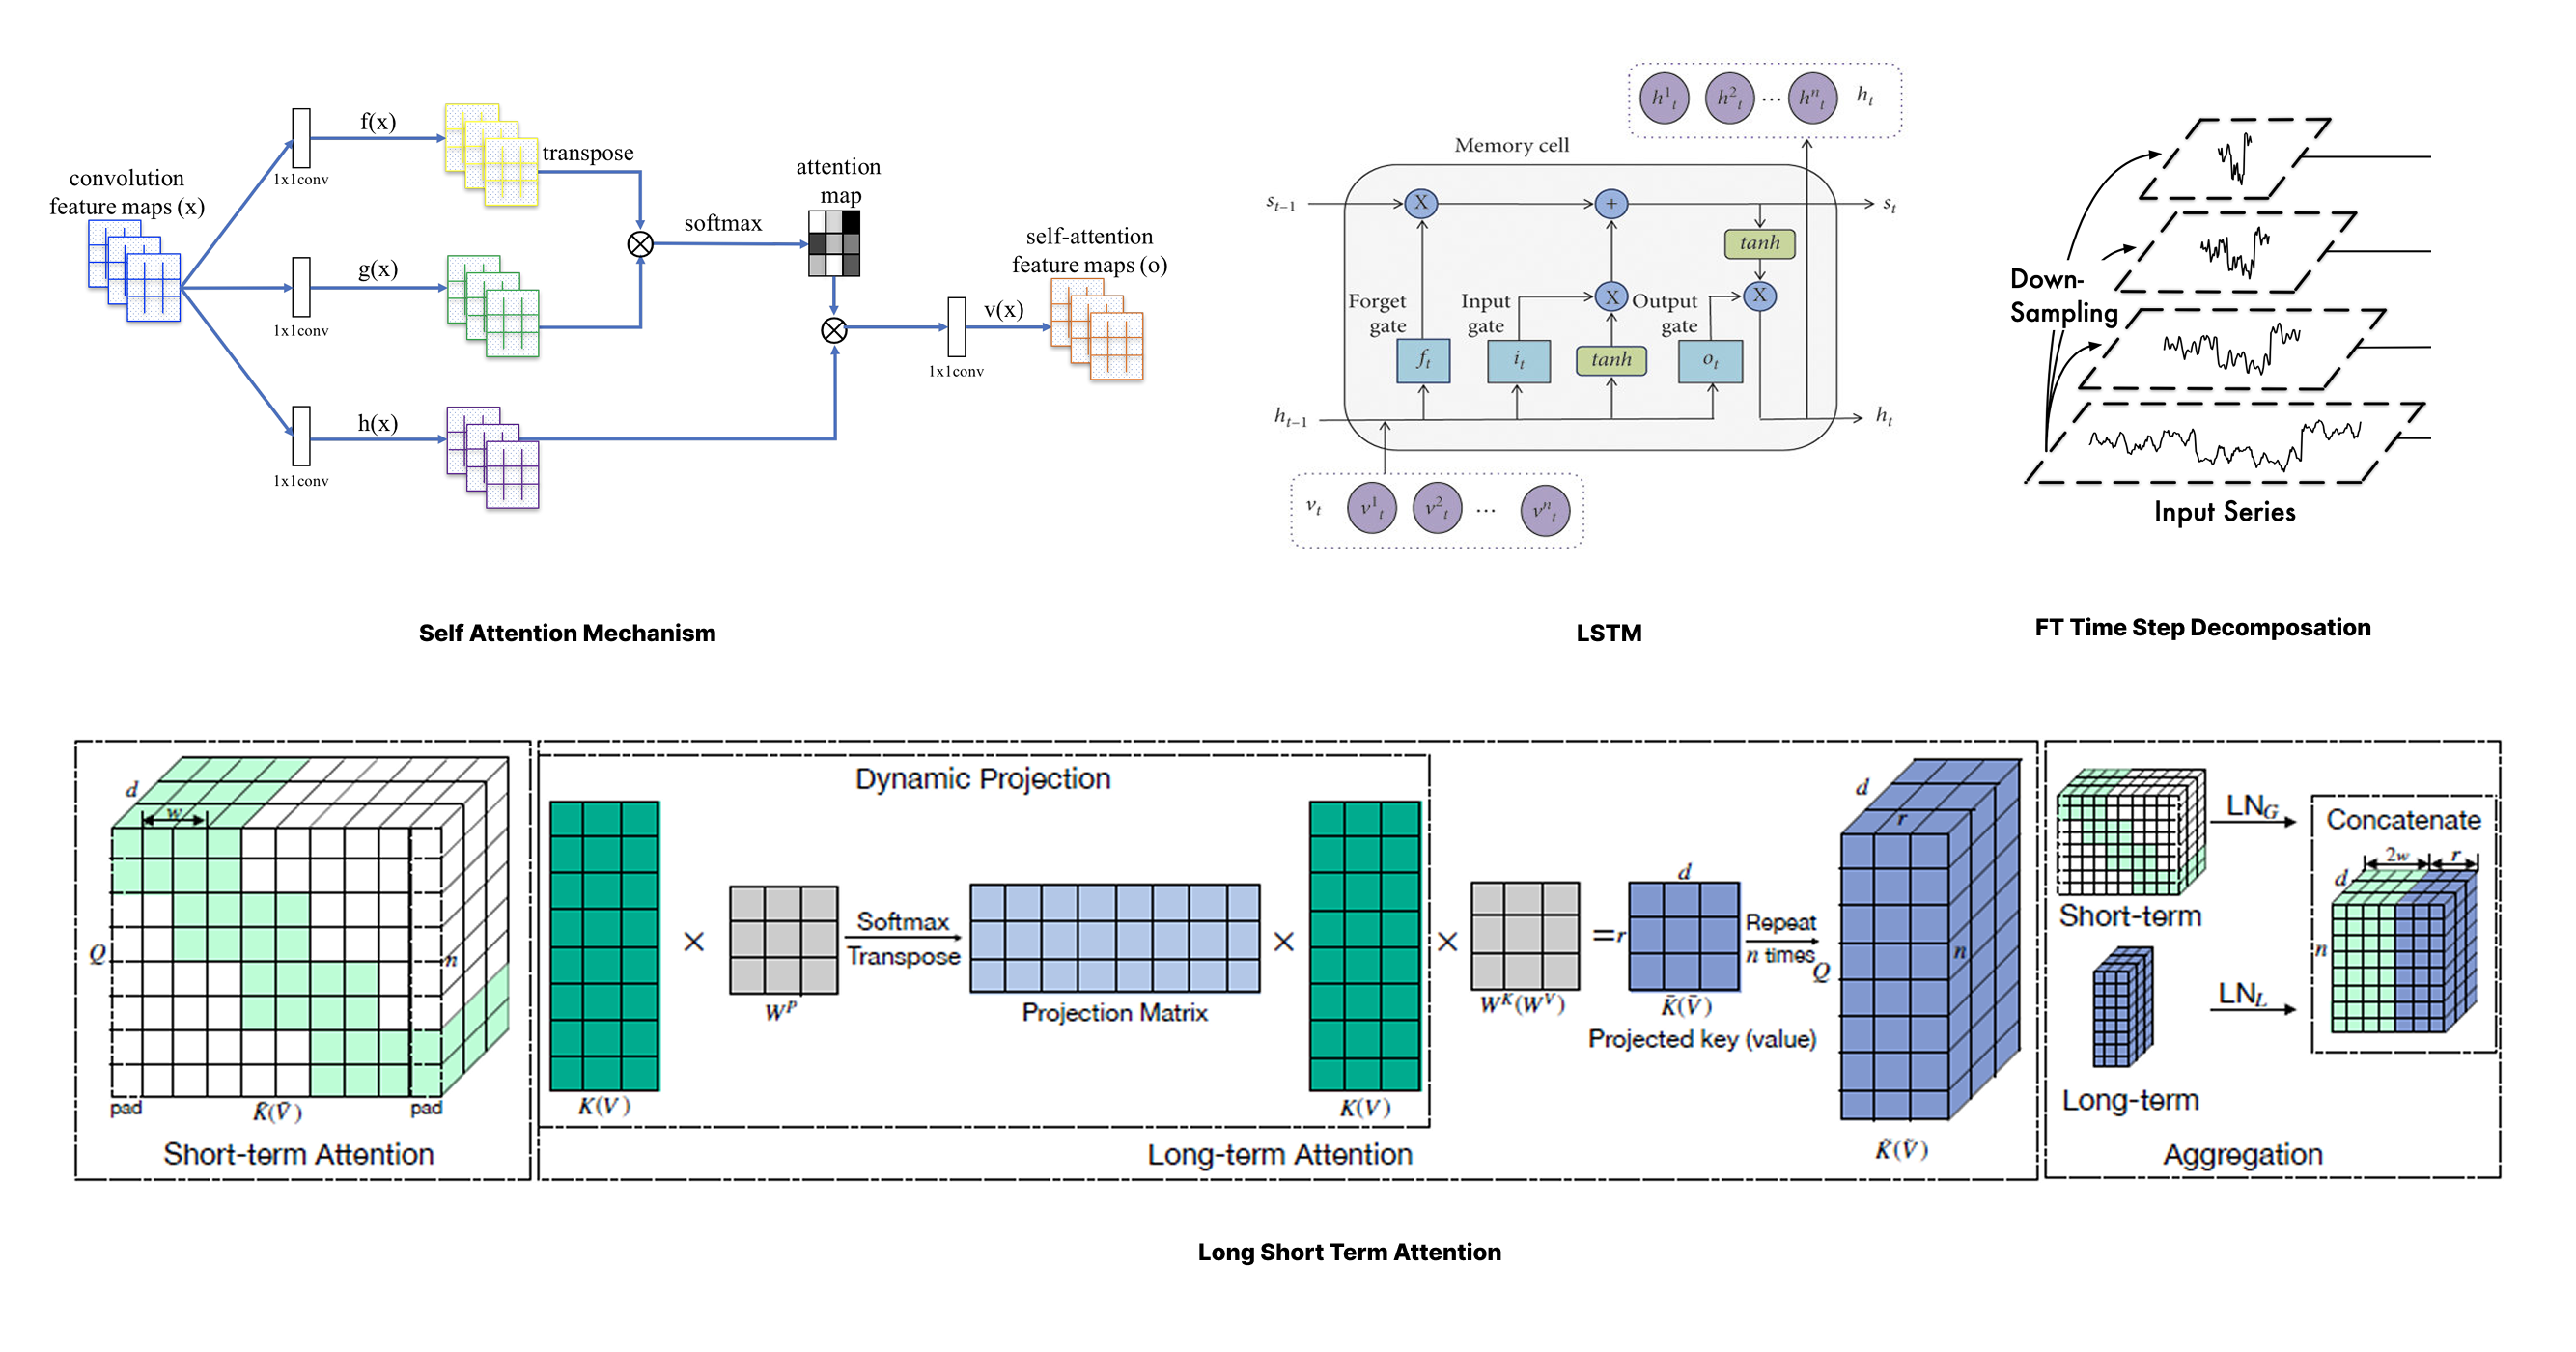
\includegraphics[width=1\linewidth]{temporal (1).png}
%     \caption{Temporal Model}
%     \label{Temporal Model}
%     \Description{Temporal Model}
% \end{figure*}
\begin{table*}[htbp]
\centering
\caption{Comparison of Deep Learning–Based Spatiotemporal Architectures for Digital Health Applications}
\label{tab:st-model-comparison}
\small
\renewcommand{\arraystretch}{1.35}
\begin{tabularx}{\textwidth}{>{\raggedright\arraybackslash}p{2.2cm} >{\raggedright\arraybackslash}p{2.5cm} >{\raggedright\arraybackslash}p{2.5cm} >{\raggedright\arraybackslash}p{1.4cm} >{\raggedright\arraybackslash}p{1.8cm} >{\raggedright\arraybackslash}X}
\toprule
\textbf{Model Type} & \textbf{Spatial Handling} & \textbf{Temporal Handling} & \textbf{Comp. Cost} & \textbf{Data Needs} & \textbf{Digital Health Examples} \\
\midrule
 
CNN-RNN Hybrid
& CNN extracts local spatial features via convolutional filters on grid-structured inputs (e.g., images, spatial maps)
& RNN/LSTM/GRU models sequential dependencies through recurrent hidden states
& Moderate to High
& Moderate; requires spatially gridded or image-like data with temporal ordering
& Medical image sequence analysis; wearable sensor forecasting; regional disease incidence prediction \\
 
\addlinespace[4pt]
 
STGNN
& GNN (GCN, GAT) propagates information over graph-structured spatial relationships (non-Euclidean)
& Temporal modules (LSTM, GRU, or temporal convolution) capture evolution along the time axis
& High
& Requires explicit graph structure (e.g., adjacency matrix); moderate to large labeled data
& Hospital network patient flow; multi-sensor physiological monitoring; epidemic spread over contact/mobility networks \\
 
\addlinespace[4pt]
 
Transformer-based ST
& Self-attention over spatial tokens or positional embeddings; no fixed spatial inductive bias
& Self-attention with temporal positional encoding captures long-range dependencies in parallel
& High to Very High
& Large-scale data preferred; benefits from pre-training; positional encoding needed for spatial structure
& Large-scale EHR longitudinal prediction; climate–health interaction modeling; multi-modal medical data fusion \\
 
\bottomrule
\end{tabularx}
\end{table*}
 
 
% Part 2: 3D-CNN and AE/SAE/VAE (continued on next page)
 
\begin{table*}[htbp]
\centering
\caption*{Table~\ref{tab:st-model-comparison} (continued)}
\small
\renewcommand{\arraystretch}{1.35}
\begin{tabularx}{\textwidth}{>{\raggedright\arraybackslash}p{2.2cm} >{\raggedright\arraybackslash}p{2.5cm} >{\raggedright\arraybackslash}p{2.5cm} >{\raggedright\arraybackslash}p{1.4cm} >{\raggedright\arraybackslash}p{1.8cm} >{\raggedright\arraybackslash}X}
\toprule
\textbf{Model Type} & \textbf{Spatial Handling} & \textbf{Temporal Handling} & \textbf{Comp. Cost} & \textbf{Data Needs} & \textbf{Digital Health Examples} \\
\midrule
 
3D-CNN \& Hybrid Networks
& 3D convolution jointly captures spatial patterns across height, width, and depth/time dimensions
& Temporal dynamics learned implicitly through the depth axis of 3D convolution kernels
& High
& High-dimensional volumetric or video-like data (e.g., $H \times W \times T$)
& Medical video analysis (e.g., echocardiography, surgical video); fMRI/brain imaging sequences; motion-based rehabilitation assessment \\
 
\addlinespace[4pt]
 
AE / SAE / VAE
& Encoder compresses spatial features into a latent space; can be combined with CNN or GNN encoders
& Temporal patterns captured when paired with sequential encoders or applied per time step
& Low to Moderate
& Can leverage unlabeled data (unsupervised / self-supervised); flexible input formats
& Anomaly detection in patient vitals; missing data imputation in longitudinal records; latent phenotype discovery from EHR \\

 
\addlinespace[4pt]

State-Space Models / Mamba
& Spatial structure handled implicitly through tokenization or combined with CNN/GNN encoders; no built-in spatial bias
& Selective state-space recurrence captures long-range temporal dependencies in linear time
& Low to Moderate
& Efficient on very long sequences; moderate labeled data
& Long continuous physiological streams (CGM, ECG, EEG); long-horizon longitudinal trajectories; long medical video \\



\bottomrule
\end{tabularx}
\end{table*}

\begin{table*}[htbp]
\centering
\caption*{Table~\ref{tab:st-model-comparison} (continued)}
\small
\renewcommand{\arraystretch}{1.35}
\begin{tabularx}{\textwidth}{>{\raggedright\arraybackslash}p{2.2cm} >{\raggedright\arraybackslash}p{2.5cm} >{\raggedright\arraybackslash}p{2.5cm} >{\raggedright\arraybackslash}p{1.4cm} >{\raggedright\arraybackslash}p{1.8cm} >{\raggedright\arraybackslash}X}
\toprule
\textbf{Model Type} & \textbf{Spatial Handling} & \textbf{Temporal Handling} & \textbf{Comp. Cost} & \textbf{Data Needs} & \textbf{Digital Health Examples} \\
\midrule

GAN
& Generator and discriminator use CNN or GNN backbones to model spatial structure
& Temporal dynamics modeled by recurrent or temporal convolution generators (conditional or temporal GAN variants)
& Moderate to High
& Augments scarce or imbalanced cohorts; benefits from moderate real samples
& Synthetic medical image and signal generation; data augmentation for rare conditions; missing value imputation \\

\addlinespace[4pt]

DDPM (Diffusion)
& U-Net (CNN) backbone captures spatial structure during iterative denoising
& Temporal or spatiotemporal dynamics modeled by conditioning the denoiser on time or sequence context
& High
& Moderate to large data; stable training with high sample fidelity
& High-fidelity medical image and signal synthesis and denoising; imputation of irregular measurements; data augmentation \\

\addlinespace[4pt]

World Model
& Encoder (CNN, GNN, or Transformer) maps observations into a latent state representing spatial context
& Latent dynamics model rolls the state forward over time for prediction and simulation
& High
& Sequential observation and action data; benefits from large interaction data
& Patient-state simulation; counterfactual intervention planning; world-model-based digital twins \\
\bottomrule
\end{tabularx}
\vspace{4pt}
{\footnotesize \textit{Note:} Computational cost is characterized relative to other architectures in this table. Actual cost depends on data scale, graph size, sequence length, and implementation details.}
\end{table*}
 
 
\subsection {Irregular Time Series and Longitudinal Modeling in Digital Health}
We include irregular time series and longitudinal modeling in this spatiotemporal survey because they form the temporal backbone of spatiotemporal modeling under real-world digital-health constraints: irregular sampling and personalized, non-stationary trajectories are precisely the temporal phenomena against which spatial and contextual covariates must be aligned, so the methods below extend rather than depart from the spatiotemporal framework developed in Sections~\ref{sec:data}--\ref{sec:history}.

Spatiotemporal models, as outlined above, have proven highly effective in capturing complex dependencies in data with spatial and temporal components. However, in digital health scenarios, additional challenges arise from non-stationary distributions, irregular sampling, and personalized trajectories. This section presents specialized methods designed to tackle these issues, including hybrid architectures for long-short term dynamics, and techniques for handling irregular time series in medical contexts. By tailoring these approaches, researchers can achieve robust and accurate predictions on real-world health datasets.

Hybrid Architecture for Capturing Long and Short Term Dependencies: Forecasting tasks often involve both short-term fluctuations and long-term trends, making it difficult for a single model to effectively capture both. The Long-Short Transformer (LST) integrates LSTM and Transformer, leveraging their respective strengths.

LSTM efficiently captures short-term variations by updating hidden states with gating mechanisms. However, its ability to model long-term dependencies is limited due to vanishing gradients. To address this, LST passes LSTM-processed features into a Transformer module, which uses self-attention to capture long-range dependencies by computing query, key, and value representations.

Self-attention enables the model to consider relationships across the entire sequence simultaneously, mitigating the limitations of recurrent architectures. By combining LSTM for local patterns and Transformer for global dependencies, LST achieves robust performance in tasks such as stock market prediction, weather forecasting, and energy consumption modeling.

\paragraph{TimeMixer: Combining Fourier Transform and Multi-Period Features}TimeMixer \cite{timemixer} processes time series using a sliding window approach, enabling the model to focus on fixed-length segments and learn both short-term and long-term periodic dependencies. Given an input sequence $X \in \mathbb{R}^{T \times D}$, where $T$ represents the number of time steps and $D$ is the feature dimension, the model applies token mixing through an MLP-based structure for temporal pattern extraction.

In addition to time-domain processing, TimeMixer incorporates frequency-domain information using the Fast Fourier Transform (FFT), which decomposes the input into frequency components:

\begin{equation}
X_f = \text{FFT}(X)
\end{equation}

where $X_f$ represents the frequency-domain representation of the input. The low-frequency components correspond to long-term trends, while high-frequency components capture short-term variations. By integrating information from different frequency bands, the model effectively enhances its ability to learn periodic patterns.

\paragraph{Trajectory-based Representation Learning and Its Relevance to Digital Health}
Recent advances in trajectory based recommendation systems provide a useful reference for spatiotemporal modeling in digital health. A representative example is the work by Yan et al., which proposes a spatio temporal hypergraph framework for next point of interest recommendation. In this setting, an individual’s historical mobility is represented as a longitudinal trajectory composed of visited locations and timestamps, and the modeling objective is to predict future behavior based on personalized spatiotemporal patterns. Although the target task is recommendation, the underlying data structure aligns closely with longitudinal health trajectories, where individual states evolve over time and across contexts.

Methodologically, the model represents user trajectories using a spatio temporal hypergraph, where hyperedges connect multiple entities such as users, locations, and time contexts. This design enables the model to capture higher order interactions beyond pairwise relationships, preserving both temporal dependency and spatial co occurrence patterns. Through hypergraph message passing, the model learns a compact latent representation of each individual trajectory, which summarizes historical behavior while retaining contextual structure. The downstream prediction task is then formulated as an optimization problem that scores candidate outcomes based on their compatibility with the learned trajectory representation.

This modeling paradigm naturally extends to digital health applications. By replacing points of interest with health related contexts such as environments, behaviors, or exposure states, and by redefining the prediction target from recommendation to disease risk or health outcome forecasting, the same spatiotemporal representation learning framework can be reused. In this view, trajectory based hypergraph models offer a principled approach for capturing personalized spatiotemporal patterns, making them a promising foundation for disease prediction and intervention modeling in digital health.

\paragraph{Multi-Scale Convolutional Network with Transformer (MICN)} MICN \cite{wang2023micn}is designed for nonlinear time series prediction by integrating multi-scale convolution with Transformer-based self-attention. The convolutional component applies filters of different sizes, where smaller kernels are effective in capturing short-term fluctuations, while larger kernels help to identify long-term dependencies. This allows MICN to extract both local and global patterns within time series data.

Once features are extracted through convolution, they are further refined using a Transformer module, which models relationships across different time steps. The self-attention mechanism assigns varying importance to different time points, effectively capturing dependencies that span across multiple scales.

By combining the strengths of convolutional networks for localized feature extraction and Transformers for long-range dependencies, MICN is particularly suited for applications such as air quality prediction, weather forecasting, and traffic flow analysis, where both short-term variations and long-term trends must be accurately modeled.

\paragraph{Periodic Transformers and Frequency-Based Models}Several Transformer-based architectures have been proposed to enhance the modeling of periodic patterns in time series: PeriFormer (Periodic Transformer): Introduces periodic encoding to capture cyclical variations, optimizing time series modeling under irregular sampling conditions. It is particularly effective in meteorological and biomedical applications.
FEDformer: Combines frequency-domain modeling with time-domain optimization to improve predictive performance, especially for strongly periodic sequences \cite{piao2024frednormer}.

Additionally, signal processing techniques such as wavelet transforms can further enhance periodic feature extraction by simultaneously analyzing temporal and spectral characteristics, providing a complementary approach to deep learning-based models.

Modeling Discrete-Time Data Features:Many real-world time series, such as medical records, sensor data, and financial transactions, exhibit irregular sampling intervals. Traditional recurrent neural networks (RNNs) assume uniform time steps, making them less effective for handling such data. Several models have been proposed to address this issue by incorporating time-aware mechanisms.

\paragraph{GRU-$\Delta t$: Gated Recurrent Units with Time Decay} GRU-$\Delta t$ \cite{metzger2023crop} extends the standard GRU by introducing a time decay factor to adjust hidden state updates based on the time interval between observations. In conventional GRUs, the hidden state is updated using reset and update gates. However, these updates assume a fixed sampling interval, making the model less adaptable to irregularly spaced data points.

To address this, GRU-$\Delta t$ introduces a decay function $\Gamma(\Delta t) = e^{-\Delta t / \tau}$, where $\Delta t$ represents the time gap between the current and previous observations, and $\tau$ is a learnable parameter that controls the rate of memory decay. When $\Delta t$ is small, the decay factor remains close to 1, preserving information from the past. Conversely, for large $\Delta t$, the decay factor approaches zero, ensuring that outdated information is gradually forgotten. This mechanism enables GRU-$\Delta t$ to handle irregular time series effectively and is widely used in medical monitoring, sensor-based forecasting, and predictive maintenance.

\paragraph{ODE-RNN: Continuous-Time Hidden State Evolution}ODE-RNN \cite{rubanova2019latent} combines neural ordinary differential equations (Neural ODEs) \cite{chen2018neural} with RNNs to model the continuous evolution of hidden states over time. Unlike conventional RNNs, which update states at fixed intervals, ODE-RNN formulates hidden state dynamics using an ODE:

\begin{equation}
\frac{dh}{dt} = f(h, t; \theta)
\end{equation}

which is solved numerically (e.g., using the Runge-Kutta method) to obtain:

\begin{equation}
h(t) = h(t_{\text{prev}}) + \int_{t_{\text{prev}}}^{t} f(h, t'; \theta) \, dt'.
\end{equation}

This approach allows hidden states to evolve smoothly between observations, making the model well-suited for irregularly sampled data. When a new observation arrives, the ODE-updated hidden state is further refined using a standard RNN update. By combining continuous-time modeling with discrete updates, ODE-RNN captures both long-term trends and sudden changes, making it applicable to ECG/EEG signal processing, financial modeling, and epidemiological forecasting.

\paragraph{Transformer-Based Models for Irregular Time Series}Several transformer-based architectures have been developed to handle irregularly spaced time series by leveraging neural differential equations and path-aware computations:
ContiFormer: Integrates neural ODEs with the Transformer framework to model continuous-time dynamics, making it effective for capturing irregular time intervals\cite{chen2023contiformer}.
Rough Transformer: Inspired by Rough Path theory, this model is designed for handling high-noise and irregularly sampled data. It computes fluctuations in unevenly spaced time series, making it particularly robust for ICU monitoring and other medical applications.

By combining time-aware mechanisms such as decay functions, differential equations, and path-based transformations, these models significantly improve the handling of irregular time series data in real-world applications.

% \begin{figure}[ht]
%     \centering
%     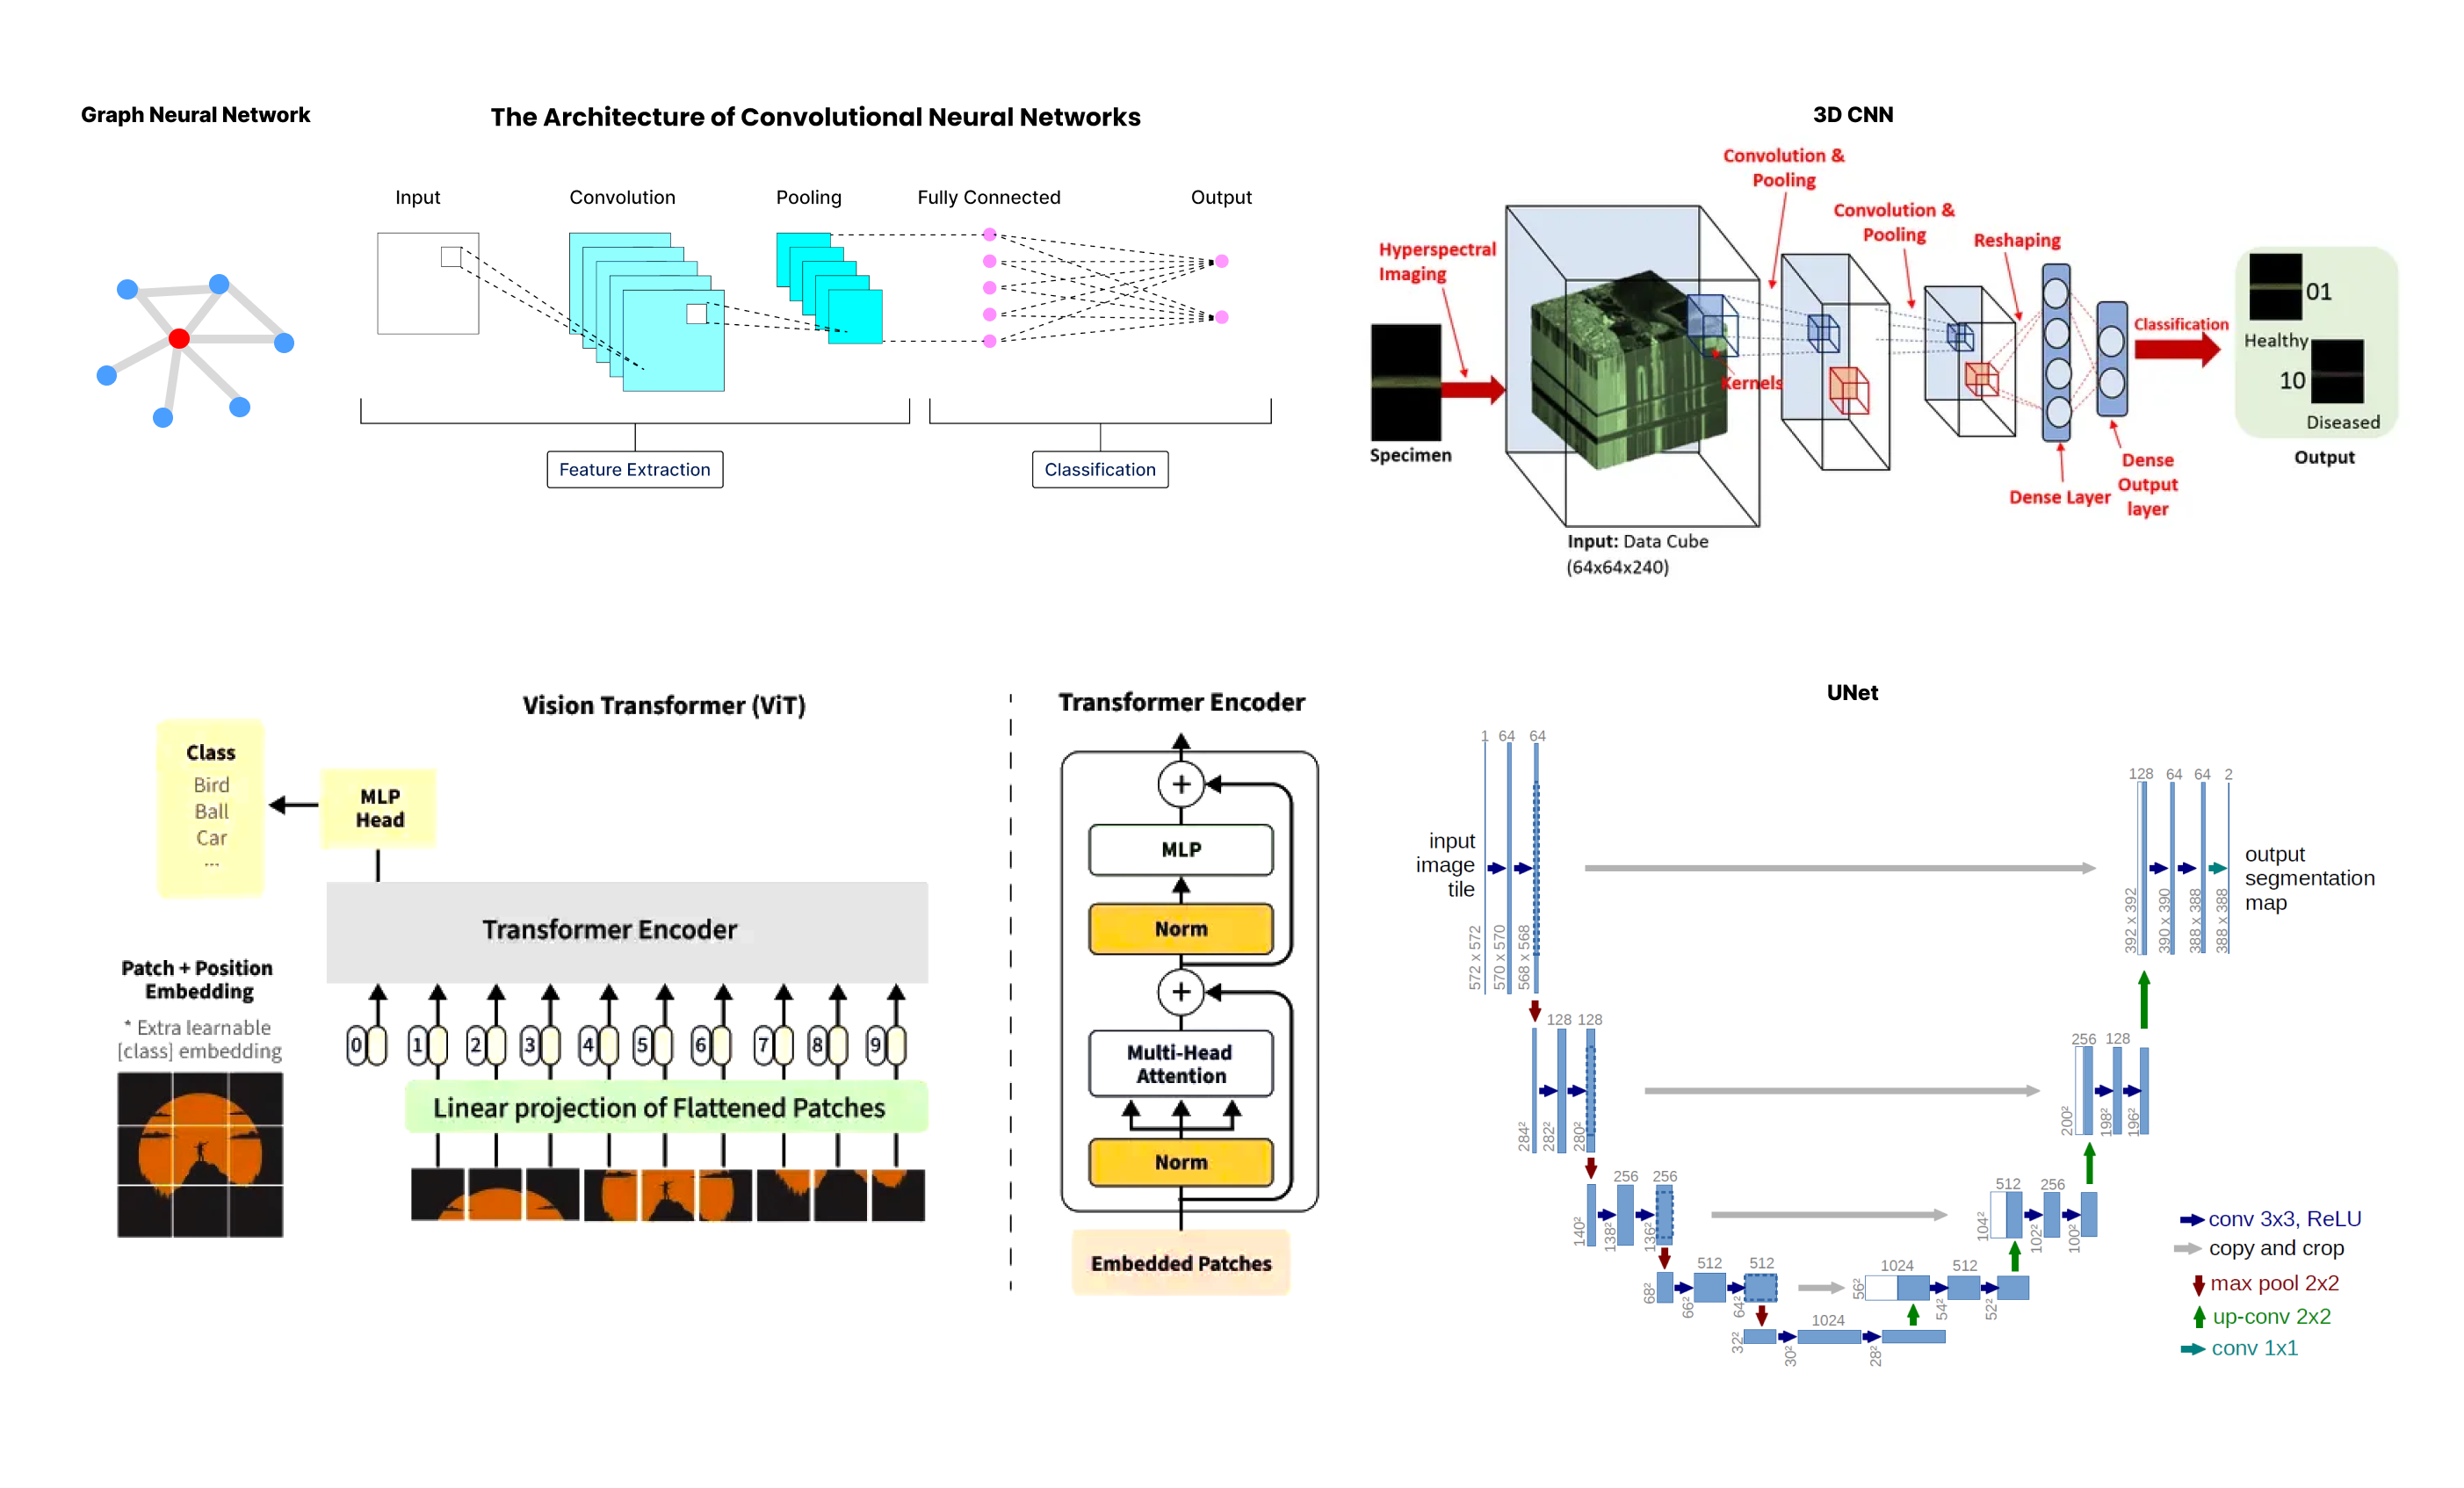
\includegraphics[width=\linewidth]{Spatio.png}
%     \caption{Spatial Model}
%     \Description{An illustration of a spatial model highlighting spatial correlations (e.g., location-based influences).}

%     \label{Spatial Model}
% \end{figure}

\paragraph{Longitudinal data analysis} Longitudinal data describes the trajectory of individuals over time, capturing both overall trends and inter-individual differences. Compared to traditional time series analysis, modeling longitudinal data requires accounting for both within-subject correlation and between-subject variability. The linear mixed-effects model (LMM) is a classical approach for handling longitudinal data, where fixed effects explain the overall trend and random effects capture individual differences. Specifically, LMM assigns random intercepts or random slopes to different individuals, allowing for personalized initial states and rates of change, thereby providing a more accurate representation of individual trajectories. However, LMM relies on linear assumptions, making it less effective when dealing with complex or nonlinear temporal patterns.  

To overcome the linearity assumption of LMM, the generalized additive mixed model (GAMM) integrates the generalized additive model (GAM) with mixed-effects modeling. It incorporates a nonlinear smoothing function, such as B-splines or P-splines, in the fixed-effects component to model temporal trends while retaining the LMM structure for random effects to capture individual differences. This enables GAMM to accommodate complex nonlinear variations in the data, making it more flexible for trend modeling. However, GAMM requires manual selection of spline basis functions and smoothness parameters, making it computationally intensive in high-dimensional scenarios. This complexity can lead to issues such as overfitting or underfitting.  

To address the limitations of GAMM in handling high-dimensional data and complex patterns, the deep generalized additive mixed model (DGAMM) replaces traditional spline functions with deep neural networks (DNN) for nonlinear mapping. By doing so, DGAMM eliminates the need for manual selection of basis functions and offers superior nonlinear modeling capabilities. The mathematical formulation of DGAMM is given by  

\[
Y_{ij} = DNN(X_{ij}) + Z_{ij} u_i + \epsilon_{ij}
\]

where \(DNN(X_{ij})\) learns nonlinear relationships automatically, while \(Z_{ij} u_i\) continues to model inter-individual random effects. Despite its advantages, DGAMM still faces challenges in long-term trend modeling. For example, DGAMM may struggle to capture long-term dependencies when processing data over extended time spans. Additionally, it lacks a dedicated mechanism for modeling individual temporal dynamics, limiting its ability to fully leverage the global structure of time-series data.  

To address these challenges, the temporal-context transformer (TCTformer) introduces both global temporal attention and personalized feature attention, leveraging the transformer architecture to enhance long-term dependency modeling while improving the representation of individual differences. The global temporal attention mechanism captures dependencies across distant time points, ensuring greater stability in health trend predictions. Simultaneously, personalized feature attention enables individualized modeling, allowing predictions to better align with unique subject trajectories. The mathematical representation of TCTformer is  

\[
Y_{ij} = TCTformer(X_{ij}) + \epsilon_{ij}
\]

TCTformer employs the transformer framework, integrating both individual-level and global temporal information, thereby overcoming the limitations of traditional methods in long-term trend prediction. Compared to LSTM or RNN, TCTformer does not rely on sequential computations, avoiding gradient vanishing issues and enabling more efficient handling of long-range dependencies. Additionally, unlike LMM, GAMM, and DGAMM, TCTformer does not require manual specification of random effects or spline basis functions. Instead, it automatically adapts to data patterns, improving modeling flexibility and generalization capabilities.  

In summary, the progression from LMM to GAMM, then to DGAMM, has successively removed constraints related to linear assumptions and manual feature selection. However, challenges remain in long-term prediction and individual feature modeling. By leveraging the transformer architecture, TCTformer provides superior capabilities in capturing long-term dependencies and personalized dynamics, opening new possibilities for longitudinal health data analysis and enabling more precise personalized health assessments and predictions.  


\section{Spatiotemporal Models in Digital Health}
\label{sec:models}
After reviewing the types of Spatiotemporal data and their downstream tasks, the subsequent sections focus on four typical application scenarios in digital health research over the past five years, namely dietary interventions, diabetes management, depression diagnosis, and cardiac disease analysis \cite{2,3,5,8}. These four domains encompass a variety of Spatiotemporal data, ranging from video-based behavior recognition and regularly sampled time-series forecasting to brain functional connectivity and cardiac imaging sequences at the 3D/4D levels, thus reflecting feature extraction and modeling requirements across different dimensions \cite{9,4}. Specifically, in the field of dietary interventions, researchers often utilize video clips or time-series sensor data to capture individual eating behavior and nutritional intake; in diabetes scenarios, the focus lies on predicting and detecting anomalies in continuously monitored blood glucose levels and area-based prevalence data; studies on depression typically involve dynamic physiological signals, such as fMRI videos or EEG, to perform high-dimensional classification and inference; meanwhile, cardiac disease analysis frequently combines 3D/4D imaging and physical priors to model the myocardium, heart chambers, or electrophysiological conduction over space and time \cite{2,5,7}. The following subsections respectively examine the data forms, the common categories of downstream tasks, and representative deep learning architectures adopted in these applications, and then provide a systematic analysis of the challenges such models encounter and future trends in their development.

\subsection{Spatiotemporal Modeling in Dietary Interventions}
Within dietary intervention and nutrition counseling, Spatiotemporal data usually appear in the form of continuous image sequences capturing exercise or eating behaviors, or as time-series sensor data transformed into ``video frames'' \cite{9}. Because such data exhibit clear temporal evolution (e.g., the duration of eating actions, posture changes, etc.) and can be viewed in terms of spatial distributions (body posture and food items within the frame), they are often treated as video data. Some studies also map environmental context and body-movement data onto a regular grid or multi-channel tensor, thus forming a raster data structure to facilitate convolution-based processing.

Regarding downstream tasks, researchers generally employ detection or classification models to recognize individual eating behaviors, or use video sequences to conduct aggregation analyses and anomaly detection \cite{9}. Such approaches not only allow for the real-time discovery of unhealthy eating patterns, but also support personalized nutrition interventions. Certain studies additionally combine external data (e.g., heart rate, activity trackers) to carry out prediction or recommendation, thereby achieving multimodal fusion.

Mainstream Spatiotemporal models often adopt a 2D-CNN plus RNN (LSTM/GRU) architecture, in which the CNN extracts spatial features from video frames and the RNN module captures temporal dependencies across frames; other research has explored 3D-CNN or ConvLSTM, which directly convolve across three-dimensional or temporal dimensions, improving the capture of continuous behavior \cite{9}. Compared to traditional methods, these architectures better handle environmental noise and variations in posture.

Nevertheless, due to the high labeling cost and the complexity of real-world situations (lighting, occlusion, individual differences, etc.), data collection and cleaning remain challenging for such applications. Future trends may include tighter integration of wearable sensors with video data to reduce the reliance on large-scale annotation via self-supervised or few-shot learning, and employing real-time inference on mobile or edge devices. The advantage of these models lies in their ability to detect subtle eating actions and support individualized interventions automatically, but the downside involves high demands on computational resources as well as the need for deeper research into explainability and cross-population generalization.

\subsection{Spatiotemporal Models for Diabetes Management and Prediction}
In diabetes scenarios, Spatiotemporal data predominantly appear as regularly sampled rasterized time-series, such as the blood glucose readings captured by continuous glucose monitors (CGMs) at fixed intervals, along with the prevalence rates of diabetes in particular regions by month or year \cite{3}. At the individual level, wearable devices or electronic health records may record personal trajectories (trajectory data) or point-referenced samples (point reference data), for example, obtaining blood glucose measurements at specific home-visit coordinates.

The key downstream tasks revolve around prediction and anomaly detection: researchers seek to predict short-term fluctuations in blood glucose from historical series or identify abrupt spikes and drops, issuing timely alerts \cite{2}. At the population level, some employ long-term time-series models of incidence in various administrative regions, aiming to forecast future prevalence rates nationally or in a particular locale for public-health policy-making \cite{3}. Additionally, certain research addresses inference or estimation, such as interpolating missing blood glucose readings or recommending individual insulin dosage based on food intake and exercise volume.

In terms of model architectures, personal-level blood glucose data are often tackled with RNN, LSTM, GRU, or attention-based Transformers to capture possible cyclical or abrupt changes in glucose \cite{2}. For region-level data, graph convolutional networks (GCNs) are utilized in conjunction with temporal modules (e.g., STGCN) to characterize inter-regional diabetes propagation or risk correlations, using geographic adjacency or social networks \cite{3}. Furthermore, some hybrid models incorporate hospital resource distribution, patient trajectory, environmental factors, and other data sources holistically.

At present, the main obstacles center on multi-source heterogeneous data fusion and privacy protection. Since the data from EHRs, wearable devices, and geographic information systems (GIS) often differ in format—and because stringent security standards exist in healthcare—real-time collection and cross-platform sharing are impeded. Future research may lie in building large-scale multimodal datasets, employing privacy-preserving methods (e.g., federated learning), and developing more intelligent personalized-adaptive models. Compared to traditional statistical methods, deep Spatiotemporal models excel at automatically learning non-linear patterns and extracting fine-grained temporal features; however, a lack of explainability, high computational demands, and possible generalization issues in new domains remain as drawbacks.

\subsection{Spatiotemporal Modeling for Depression Diagnosis and Intervention}
In depression research, fMRI video sequences and EEG time-series represent two common forms of Spatiotemporal data \cite{2,4,5}. For population-level disease statistics, these data may be viewed as a fixed grid of continuously sampled raster data, e.g., monthly or annual counts of confirmed diagnoses \cite{3}. If investigators must describe the functional connectivity topology between neurons or brain regions, they often construct a dynamic functional connectivity (dynamic FC) graph evolving over time \cite{4,5}.

Downstream tasks typically include classification (distinguishing between patients with depression and healthy controls \cite{2,5}), detection (identifying abnormal brain activity), inference or estimation (filling in missing segments of signals), as well as larger-scale prediction (e.g., predicting depression case counts in the next time window using national-level data \cite{3}). Additionally, for specific patients, there may be tasks related to predicting treatment response or clinical prognosis \cite{4,5}.

The choice of Spatiotemporal model depends substantially on the data type: for fMRI video sequences (video data), researchers often leverage 3D-CNN, ConvLSTM, bidirectional ConvLSTM U-Net, etc., to capture both spatial-anatomical structures and temporal changes (e.g., over a cardiac or neural cycle) \cite{7,8}. For one-dimensional EEG time-series, CNN + GRU/LSTM is commonly employed to model both frequency and temporal dependencies \cite{2}. When handling dynamic brain connectivity networks, it is feasible to combine a graph convolutional network (GCN) with an RNN, forming an STGCN; or to use attention mechanisms to highlight interactions between critical brain regions \cite{4,5}.

A key challenge in this domain is the inherently high-dimensional yet small-sample nature of fMRI/EEG data: each subject can produce huge amounts of Spatiotemporal data, yet due to scanning expense and ethical limitations, total sample sizes may only number a few hundred \cite{4,5}. Moreover, merging data across multiple centers introduces heterogeneity in scanning equipment and protocols, making cross-domain generalization extremely difficult. Future directions include small-sample or self-supervised learning approaches, multimodal fusion (integrating imaging, behavioral, and genetic data), and more flexible distributed or federated training. While these methods can autonomously capture complex neural patterns or the population spread of disease—thus aiding individual-level diagnosis and public-health forecasting—significant obstacles remain, such as data scarcity, privacy constraints, and the need for interpretable models before reaching clinical deployment.

\subsection{Spatiotemporal Modeling in Cardiac Diseases}
Research on cardiac diseases primarily involves cardiac imaging sequences (e.g., MRI, CT, echocardiography) along with signals from ECG or intracardiac leads \cite{6,7,8}. Cine-MRI or ultrasound sequences are often regarded as video data that can be used by segmentation or detection models to dynamically identify myocardium or cardiac chambers. ECG and lead signals, on the other hand, are time-series that may be mapped onto discrete spatial nodes to form raster data or Spatiotemporal graphs \cite{8}.

Typical downstream tasks include segmentation and detection (automatically delineating cardiac anatomical structures or lesions \cite{6,7,8}), classification (e.g., detecting arrhythmias or heart failure), prediction (anticipating future cardiac function indicators or clinical risks), and inference (employing physical priors to model the Spatiotemporal propagation of electrical signals \cite{8}). Some studies adopt multi-task learning to combine segmentation with functional estimations or lesion identification.

Commonly used Spatiotemporal models include 3D-CNN and ConvLSTM (as well as variants like bidirectional ConvLSTM U-Net), which directly apply spatial convolution and temporal recurrences to multi-frame cardiac sequences; for electrical signals, LSTMs or Transformers are employed to capture long-range temporal dependencies \cite{6,7}. When representing cardiac electrophysiological topologies, researchers often introduce GNNs or physics-informed deep learning to enhance the precision of conduction modeling \cite{8}.

Challenges in this area primarily arise from center-to-center variations in scanning protocols and instrumentation, which cause inconsistencies in labels and degrade out-of-domain performance; also, high-resolution cardiac imaging significantly increases training overhead, and real-time demands in clinical settings necessitate rapid inference speeds \cite{7}. With improved hardware performance and broader multi-center collaborations, future developments are likely to explore more lightweight and interpretable models, potentially combining physical priors with multimodal data (e.g., ECG, imaging, genetics) to boost accuracy and robustness. Although such techniques allow a fine-grained capture of cardiac motion and pathological evolution, they also require high-quality data and robust training environments, posing barriers for deployment across diverse clinical domains.

\subsection{Cross Domain Patterns in Spatiotemporal Modeling for Digital Health}
Across the four application domains above, several recurring patterns clarify how spatiotemporal modeling choices map onto the data forms and clinical tasks of digital health; we synthesize them below as practical guidance for selecting and deploying spatiotemporal models
\paragraph{Cross-domain versatility and adaptability.}
In dietary interventions, diabetes management, depression diagnosis, and cardiac disease scenarios, researchers frequently adopt CNN- or GCN-based networks coupled with time-series modules (LSTM/GRU/Transformer) or Spatiotemporal graph convolutional networks (STGCN) to jointly model spatial and temporal information \cite{2,3,4,6}. Such approaches are effective across diverse data types (video sequences, raster data, EEG time-series, etc.). For instance, in depression research, functional connectivity analysis often integrates anatomical priors \cite{4}, whereas cardiac disease research uses physical equations to describe blood flow or cardiac electrophysiology \cite{5,7}. Although each application area emphasizes distinct details, the fundamental principle remains the unified modeling of spatial dependencies and temporal evolution.

\paragraph{The bottleneck of small sample sizes coupled with high-dimensional data.}
Neuroimaging data (fMRI/EEG) and cardiac imaging data (4D MRI/CT) are both high-resolution and high-dimensional. However, feasible sample sizes remain small due to expensive data collection and ethical constraints, making models prone to overfitting and poor domain transfer \cite{4,5,6}. Some efforts seek to mitigate data scarcity through physical priors \cite{7}, active learning, or multi-center collaboration (federated learning). For example, in studies with limited fMRI data for depression, self-supervised or attention-based mechanisms can pinpoint critical brain regions, preventing the model from being overwhelmed by universally high-dimensional input \cite{2,4}.

\paragraph{Multimodal fusion and external knowledge.}
An increasing number of studies integrate heterogeneous data sources—environmental factors, exercise, genetics—alongside the principal Spatiotemporal signals, resulting in more comprehensive assessments of health status \cite{2,3}. In the diabetes context, the combination of blood glucose monitoring and geographical statistics yields risk maps of disease prevalence \cite{3}, whereas in cardiac research, incorporating physiological or physical models can boost interpretability and modeling accuracy \cite{5,7}. These so-called ``deep learning + clinical or physics-based priors'' methods enhance the overall model capacity and offer more feasible clinical applications.

Recent statistics-journal work reinforces this direction by showing how domain constraints and uncertainty models can be formalized before or alongside neural representation learning. For example, stochastic convection--diffusion and dynamic-deformation models encode physical transport and nonstationary spatial dependence, while spatiotemporal disease-mapping and spatial SIR emulator models demonstrate how Bayesian hierarchical structure can connect environmental exposure, regional health outcomes, and temporal disease dynamics~\cite{liu2022convectionDiffusion,castroMorales2025dynamicDeformation,wang2024respiratoryDiseaseMapping,trostle2024spatialSIR,wikle2023statisticalDeepLearning}.

\paragraph{Real-world deployment in clinical and public health contexts.}
Some studies have shifted from individual level diagnostics to broader macro scale analyses, such as long term predictions of diabetes or depression at the regional or city level, in order to assess the geographic spread and temporal trends of these diseases \cite{3}. However, this approach requires socioeconomic factors, transportation networks, and population mobility to be incorporated into spatiotemporal frameworks. In practice, uncertainty in defining geographic adjacency, together with data noise, can hinder robust model performance \cite{2,3}.

\paragraph{Increasing attention to computational efficiency and resource consumption.}
With Spatiotemporal data experiencing continual upscaling in resolution and sampling frequency, model training and inference carry higher computational overhead \cite{5,7}. Some researchers pursue network compression, edge computing, or hardware-software co-optimization to ensure real-time or near-real-time outputs, especially vital for continuous health monitoring (e.g., frequent blood glucose checks, dynamic cardiac supervision).

\paragraph{Demands for explainability and standardization.}
In clinical fields like cardiology or neuroscience, the call for deeper explainability in advanced models is growing \cite{4,6}. Visualization via attention maps or highlighting crucial time-space segments can help specialists validate or interpret diagnostic decisions \cite{2,4}. Moreover, data collection and labeling methodologies often lack consistency across centers, limiting model reproducibility \cite{6}. Scaling Spatiotemporal modeling to large-scale clinical usage thus requires further work on data governance, consistent annotation protocols, and established benchmarking.

\section{ DNN-based Medical Models and Longitudinal Models}
\label{sec:categorization}
Whereas the previous section organized spatiotemporal models by clinical application domain, this section turns to the complementary family of DNN-based medical and longitudinal models, organized around the modeling task---dynamic prediction and risk stratification---rather than the disease area.

In this section, we explore a range of advanced deep learning frameworks that have been developed to address the challenges of dynamic prediction and risk stratification in medical applications. These models leverage longitudinal data—from multivariate clinical measurements to sequential imaging scans—to capture temporal trends and complex non-linear interactions. By integrating diverse architectures such as MFPCA, CNNs, transformers, and recurrent networks, the reviewed methods provide innovative solutions for predicting survival outcomes, assessing long-term mortality risk, and improving personalized patient care.

\subsection{Deep Learning for Dynamic Prediction of Multivariate Longitudinal and Survival Data}
Lin et al. ~\cite{lin2022deep} propose a novel deep learning framework that jointly models multivariate longitudinal data and time-to-event outcomes. Traditional joint models often rely on restrictive parametric assumptions and encounter computational challenges when incorporating multiple longitudinal measures. To address these issues, the authors review and compare several methodologies:

MFPCA-based Approaches:
    The paper first discusses methods that use multivariate functional principal component analysis (MFPCA) to extract key features from longitudinal data. These features are then integrated into survival models such as the Cox model (MFPCA-Cox) and its deep learning variant, DeepSurv (MFPCA-DeepSurv). While computationally efficient, these approaches may not fully capture complex non-linear interactions.
    
CNN-based Method (MATCH-net): 
    MATCH-net adapts convolutional neural networks (CNNs) to handle the sequential nature of clinical data, effectively addressing irregular sampling and missing values. This model directly predicts survival probabilities but does not concurrently forecast future longitudinal trajectories.
    
Transformer-based Method (TransformerJM):
    The core contribution of the paper is TransformerJM, which leverages the transformer architecture for joint modeling. By treating each patient visit as a token in a sequence, the model employs masked multihead self-attention and positional encoding to capture temporal dependencies. This end-to-end framework not only predicts future longitudinal measurements but also dynamically updates survival probabilities as new data become available. TransformerJM is shown to excel in scenarios with non-linear interactions and non-proportional hazards.

\subsection{Deep Learning Approaches for Long-Term Mortality Risk Stratification in Liver Transplant Recipients}

Recent advances in deep learning have been applied to address the challenge of long-term mortality risk stratification in liver transplant recipients. In the study by Nitski et al. \cite{nitski2021long}, the authors developed and validated a series of deep learning models that leverage longitudinal clinical data to forecast patient outcomes over both short-term (1-year) and mid-term (5-year) horizons. Traditional risk models in liver transplantation predominantly rely on static logistic regression, focusing on the most recent clinical measurements alone. This overlooks the dynamic nature of post-transplant follow-up data as well as potential non-linearities among numerous clinical variables. By incorporating longitudinal data to update mortality risk predictions on a continual basis, the proposed framework addresses these limitations.

The authors compared several deep learning architectures: a simple Multilayer Perceptron (MLP) baseline, a Recurrent Neural Network (RNN) to capture temporal dependencies, a Temporal Convolutional Network (TCN) that employs convolutional filters for time-series feature extraction, and a Transformer model utilizing self-attention mechanisms to model long-term dependencies. The Transformer achieved the highest AUROC values and outperformed both conventional logistic regression and other deep learning methods. Model development relied on a large dataset from the Scientific Registry of Transplant Recipients (SRTR), and external validation took place using data from the University Health Network (UHN). A transfer learning strategy further fine-tuned the best-performing model (the Transformer) on the UHN dataset to improve generalizability. Performance metrics were based on AUROC, with the Transformer showing significant gains over baseline models.

The clinical implications are notable because this dynamic deep learning approach incorporates new follow-up data as it becomes available, allowing for real-time risk stratification. By more accurately identifying patients at elevated risk of mortality, clinicians can tailor post-transplant care strategies to prevent adverse outcomes and potentially improve overall transplant success rates.


\subsection{Deep Learning for All-Cause Mortality Prediction from Longitudinal DXA Imaging}

Glaser et al. \cite{glaser2022deep} address the challenge of predicting all-cause mortality by leveraging longitudinal total-body DXA imaging. Traditionally, mortality models based on body composition have relied on summary metrics extracted from imaging data; however, such approaches often overlook the rich, raw information present in DXA scans and the temporal changes in body composition. The authors propose and test two key hypotheses:

 Feature Extraction from Raw Imaging: Deep neural networks can automatically extract predictive features directly from raw DXA scans. These features, whether used alone or in combination with traditional clinical risk factors, improve the prediction of all-cause mortality.

Longitudinal Modeling: Sequence models, such as recurrent neural networks (e.g., LSTM), which process multiple DXA scans over time, outperform models that rely on a single scan. This approach captures the temporal evolution of body composition, leading to enhanced predictive performance.


To test these hypotheses, the study develops several architectures:

 \paragraph{Single-record models} utilize a DenseNet121 network to process image crops from the DXA scans, a fully-connected network for clinical metadata, and a combined-modality model that fuses both feature sets.
 
 \paragraph{Sequence models} treat the longitudinal data as a time series by extracting embeddings from each visit and processing these via an LSTM network to capture temporal dependencies.


\section{Spatiotemporal Models in Medical Digital Twins}
\label{sec:DT}
The preceding sections reviewed the development trajectory and key techniques of spatiotemporal models in digital health, yet bringing them into real-world clinical workflows still faces several practical constraints. Along the typical pathway of “symptom perception—clinic visit—diagnostic testing—treatment—rehabilitation,” diagnosis and treatment are the core of decision making; however, three issues remain salient: (1) Insufficient data collection and individual heterogeneity: reliance on patient recall and self-report often leads to information gaps and inconsistent time labels, which fundamentally limits a model’s ability to learn long-term dependencies and cross-modal associations. Building on this, differences in constitution, lifestyle, and social environment give rise to pronounced heterogeneity in clinical data; multifactorial etiologies and their interactions further mean that no single variable can fully explain disease trajectories. How to comprehensively collect heterogeneous information and achieve effective data fusion remains an open problem. (2) Data security and privacy: model training and individualized prediction must balance utility with privacy protection—on the one hand, fully leveraging highly sensitive health information, and on the other, meeting stringent compliance and security requirements. (3) Data presentation and interpretation: whether model outputs can be communicated to clinicians and patients accurately and efficiently directly determines clinical interpretability and usability; faced with diverse and interdependent data types, achieving multidimensional integration and intuitive presentation is a key challenge across the entire application pipeline.

Against this backdrop, digital twins offer a coherent, integrated solution to the above three challenges. The core concept is to construct, in virtual space, a “human mirror” that links to the individual in real time or near real time, serving as a hub that continuously aggregates and governs multisource time-series data from wearable devices (e.g., smart bands, smartphones) and fixed medical equipment (e.g., continuous glucose monitors, MRI), enabling cloud-based standardization, temporal alignment, and cross-modal fusion. At the population level, large-scale longitudinal observations provide spatiotemporal models with broader sample coverage and richer representations of inter-individual variation, thereby improving predictive accuracy and generalization while furnishing a more complete evidence base and case support for clinical practice. Furthermore, privacy-enhancing techniques such as federated learning enable model training under “data remain in place” constraints, balancing performance with data confidentiality. Finally, the digital twin’s multidimensional visualization and human-in-the-loop mechanisms can present both intermediate representations and final predictions in structured, interpretable forms to clinicians and patients, facilitating a closed loop of decision support and self-management. In what follows, we elaborate on data acquisition and fusion, privacy-preserving modeling, and clinical visualization and interaction.

\subsection{Digital Twin in Digital Health}

A Digital Twin (DT) is a cyber–physical feedback loop in which real-time, multimodal data from sensors and IoT devices stream to a high fidelity virtual replica, are analyzed, and then fed back to the physical asset for actuation or decision making. The concept originated in aerospace and manufacturing, where it supports the full product life cycle—including design, simulation, monitoring, and maintenance—to reduce development costs and prevent catastrophic failures \cite{Tao2018}. In healthcare, the emphasis shifts to the runtime phase. Four functional tiers are widely recognized: visualization and monitoring, prediction, optimization, and closed loop control, as outlined in the NIST digital twin framework and recent healthcare digital twin reviews \cite{NIST2021,sun2023digitaltwin}. De Kerckhove further argues that the most advanced form of a digital twin is the personal digital twin \cite{deKerckhove2021}.

Personal twin fuse continuous glucose monitors, wearables, home IoT and genomics to drive patient specific models. Faruqui \emph{et al.}\ applied transfer learning to a neural network and paired it with a clinician guided feedback controller to generate daily, personalized lifestyle recommendations for managing type 2 diabetes; prediction accuracy exceeded eighty percent and produced sustained improvements in HbA1c blood test result and weight \cite{Faruqui2024}. Silfvergren \emph{et al.} built a multi‑organ metabolic model that personalises fasting schedules and macronutrient ratios by simulating hepatic glycogen turnover \cite{Silfvergren2022}. For cardiovascular care, continuous PPG and ECG streams injected into cardiac twin detect atrial fibrillation and impending de‑compensation, reducing readmissions \cite{Bayoumy2021,Williams2023}. Because personal twin rely on high‑frequency, privacy‑sensitive data, they are increasingly paired with federated learning and differential‑privacy mechanisms.


\subsection{Challenges in Data Collection and Prediction for Medical Digital Twins}

In the construction of medical digital twins, data collection is both the most fundamental and one of the most challenging stages. The main difficulty arises from the diversity of data sources. In medical contexts, data originate from electronic health records (EHR), medical imaging (CT, MRI, ultrasound), laboratory test results, physiological signals captured by wearable devices, and real-time monitoring data from ICU systems. These different sources exhibit significant disparities in sparsity and sampling rates: for example, EHR records are sparse and infrequent, whereas ICU monitoring devices capture data at millisecond or second-level granularity; imaging data are usually interval based snapshots that fail to fully capture dynamic processes. Such heterogeneity leads to inconsistencies across temporal, spatial, and semantic dimensions, thereby increasing the difficulty of data alignment and integration.

Moreover, there are substantial differences between modalities, such as textual medical records versus imaging data, or structured laboratory indicators versus continuous physiological signals. Addressing the integration of heterogeneous multimodal data remains a key challenge in the implementation of digital twins in healthcare. Previous studies have pointed out that the standardization and fusion of multi-source heterogeneous medical data are prerequisites for achieving accurate digital twins\cite{tao2019digital,reddy2015healthcare}.

In the prediction stage of digital twins, leveraging multimodal data to achieve higher predictive accuracy is a research hotspot. Single modality data often fail to comprehensively represent a patient’s state; for instance, relying solely on electrocardiograms to predict cardiac events may be vulnerable to noise or missing values. Multimodal prediction methods can exploit the complementarity of different data sources, such as combining physiological signals, laboratory test results, and imaging information to construct patient specific digital twins that more accurately simulate disease progression. Multimodal learning frameworks can perform cross-modal feature alignment and information fusion, effectively mitigating the impact of sparsity and single-point failures~\cite{baltrusaitis2019multimodal}. For example, deep learning–based multimodal fusion models have demonstrated significant advantages in cardiovascular disease prediction, outperforming unimodal models in both predictive accuracy and robustness~\cite{huang2020fusion}. Therefore, the prediction stage of digital twins should incorporate as much multimodal and multi-source data as possible to enhance generalizability and clinical applicability.

Another major challenge in constructing medical digital twins lies in patient heterogeneity, which complicates precise disease prediction. Variability among patients not only arises from demographic factors (such as age, sex, and ethnicity), genetic background, and environmental exposures, but also from disease subtypes and individualized trajectories. Identical physiological indicators may have different clinical implications across patient populations; for example, the same BMI or blood pressure level may correspond to varying health risks in different ethnic groups. If such heterogeneity is not adequately modeled, systematic bias may occur, reducing the reliability of predictions in clinical applications~\cite{obermeyer2016predicting,rajkomar2019machine,yu2018artificial}. To address this, researchers have proposed introducing individual prior information into predictive modeling, such as baseline characteristics, genetic information, and medical history, to build patient specific digital twins. This approach enables the model to account for individual differences during prediction, thus improving specificity and robustness~\cite{bjornsson2020digitaltwins}. Methods based on Bayesian inference or meta learning can leverage small amounts of patient specific data to quickly adapt model parameters, making the digital twin more reflective of the real patient.

Beyond predictive accuracy, patient heterogeneity also significantly impacts model interpretability. Large distributional differences between individuals can lead to highly complex decision boundaries, making it difficult for clinicians to understand the basis of predictions. This ``black box effect'' undermines trust in clinical settings, thereby limiting real-world adoption~\cite{rudin2019stopexplaining}. Studies have shown that interpretability is as important as accuracy in medical AI, especially in high risk scenarios such as oncology, cardiovascular disease, and intensive care, where clinicians favor models that provide transparent reasoning processes~\cite{tonekaboni2019clinicians,lundberg2017unified}. The goal of digital twins is not only to replicate and predict patient health states but also to support clinical decision making. Thus, models must not only predict disease risk or progression accurately but also explain why a given prediction is made. This is crucial for physician understanding, trust, patient communication, and compliance~\cite{voigt2021digital}. Recent work has proposed various approaches to improve interpretability, such as attention based feature weight visualization, post hoc explanation methods (SHAP, LIME), and causality driven models integrating medical knowledge graphs, all of which contribute to improving transparency in medical digital twins~\cite{ahmad2018interpretable}.


\subsection{Medical Data Privacy Problem and Federated Learning in Digital Twin} 

\paragraph{Why medical data privacy is critical.} Data breaches and cybersecurity attacks in the healthcare sector have led to a wide range of consequences. First, identity theft and fraud occur frequently because healthcare data contains extensive personal information (such as Social Security numbers, insurance details, and medical histories), which is often more valuable on the black market than typical financial data.\cite{Seh2020HealthcareDataBreaches,Choi2021CybersecurityRisks} For example, in 2015, the Anthem Inc. data breach exposed nearly 80 million patient records, resulting in numerous fraudulent insurance claims. Second, ransomware attacks have become a prevalent threat to healthcare organizations, in which attackers encrypt patient data and demand ransom payments.\cite{Nemec2024HealthcareSecurity,Ronquillo2018HealthITHacking} One of the most notable examples is the 2017 WannaCry attack, which severely affected the United Kingdom’s National Health Service (NHS) and led to delays in surgeries and emergency services. Moreover, psychological and physical harm to patients should not be overlooked. Once sensitive health records (such as HIV status or psychotherapy notes) are exposed, patients may face social stigma, psychological distress, or even extortion by criminals.\cite{McLeod2018CyberAnalytics,Okafor2023CybersecurityUSHealthcare} In 2021, for instance, Finland’s psychotherapy center Vastaamo was hacked, and numerous patients were threatened with the publication of their therapy records, causing widespread fear. Another serious concern is medical identity theft, which can alter or confuse the original medical history and lead to misdiagnosis or improper treatment—such as adverse drug reactions—potentially resulting in death.\cite{Coventry2018CybersecurityHealthcare} At the same time, healthcare institutions face enormous financial losses. According to one report, the average cost of a data breach in the healthcare industry has reached USD 10.1 million per incident.\cite{Argaw2020HospitalCybersecurity} For example, in 2022, Scripps Health in San Diego, California, was hit by a cyberattack that prevented access to patient records and resulted in millions of dollars in losses. In general, medical data, by its very nature, is highly sensitive. Traditional security models that rely on centralized data storage have proven vulnerable to cyberattacks and breaches, compromising patient privacy. Recent research highlights the limitations of these conventional approaches and proposes enhanced security methods such as blockchain and differential privacy techniques. Rieke et al. discuss the privacy challenges inherent in digital health and introduce federated learning as a secure data sharing alternative \cite{rieke2020digitalhealth}. Similarly, Dhiman et al. compare federated learning with traditional security methods, emphasizing its potential to reduce risks associated with centralized storage \cite{dhiman2022FL}. \begin{figure}[ht] \centering 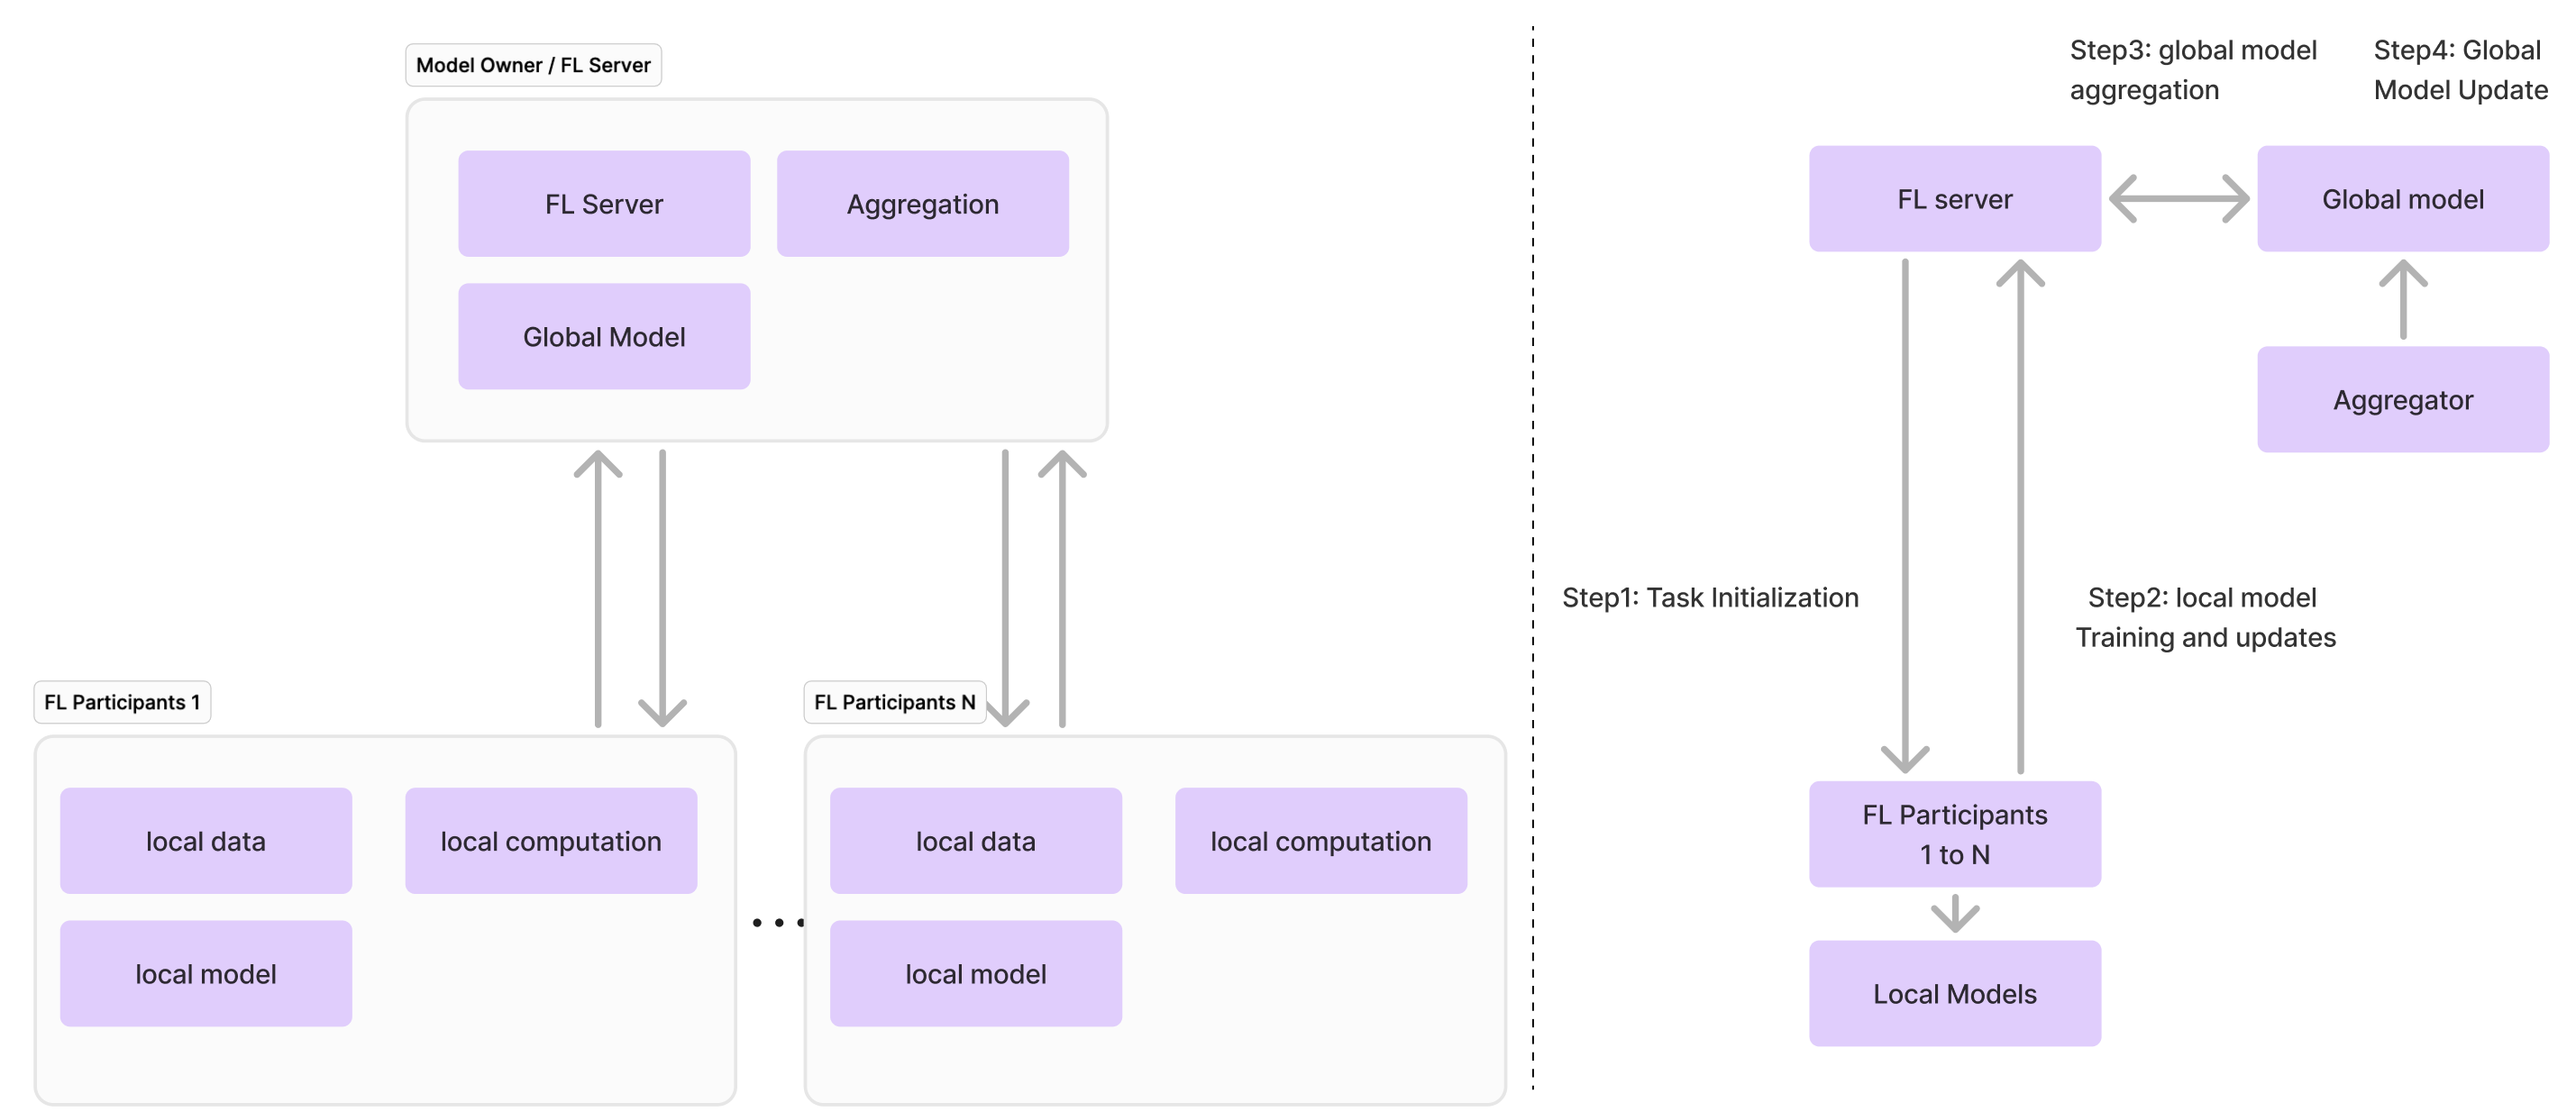
\includegraphics[width=\linewidth]{Screenshot 2025-02-28 at 11.06.26 AM.png} \caption{The federated learning training cycle: a global model is distributed to participating institutions, each trains it locally on its own private data, and only the resulting model updates are returned to a central server for aggregation, so raw patient data never leave the institution.} \Description{A schematic of the federated learning process, showing local training on multiple clients and global aggregation of model updates on a central server without sharing raw data.} \label{fig:Federated Learning Process} \end{figure}

\paragraph{How federated learning works.} Federated Learning offers a decentralized approach to machine learning, whereby multiple institutions can collaboratively train a model without transferring their raw data. Instead of sending sensitive patient information to a central server, FL enables training to occur locally on each institution’s dataset, exchanging only model updates while maintaining data privacy. Federated learning comprises four steps, shown in Figure~\ref{fig:Federated Learning Process}: (1)~\emph{Initialization:} a global model is initialized and sent to all participating clients; (2)~\emph{Local Training:} each client trains the model using its local data, computing updates rather than sharing raw information; (3)~\emph{Model Aggregation:} the locally trained models are encrypted and transmitted to a central aggregator (or decentralized peers), where updates are combined; and (4)~\emph{Global Model Update:} the aggregated updates refine the global model, and the process repeats iteratively. This method not only addresses privacy concerns but also helps institutions comply with regulatory frameworks like HIPAA and GDPR. However, FL faces challenges such as communication overhead, handling non-independent and identically distributed (non-IID) data, and defending against adversarial attacks. A systematic review by Prayitno et al. \cite{prayitno2021FLhealthcare} presents various FL implementations in healthcare, focusing on issues related to data partitioning and privacy. Coelho et al. further evaluate the security risks intrinsic to FL models, advocating for robust measures to counter potential cyber threats \cite{coelho2023FLsecurity}.


\paragraph{Federated learning for spatiotemporal models in digital twins.} Integrating federated learning (FL) with Spatiotemporal (ST) longitudinal models inside a digital twin (DT) framework creates a privacy‑preserving pipeline that ingests heterogeneous sensor streams, updates patient‑specific twin continuously, and distributes population‑level insights across institutions without moving raw data \cite{aouedi2022FLmedical}. In a typical workflow, local twin running on edge devices or hospital servers encode multivariate ST trajectories—such as diet logs, continuous‑glucose‑monitoring traces, and region‑dependent lifestyle factors—into latent representations. Each site refines a shared ST deep‑neural network on its private longitudinal cohort and transmits only encrypted model updates to a central aggregator. The aggregated parameters are redistributed, synchronizing thousands of twin while staying compliant with data‑protection regulations (see Fig.~\ref{fig:architecture of FL}).  From a DT life‑cycle perspective, FL chiefly enhances the stages of personalized model optimization and real‑time monitoring by letting each twin learn from a much larger virtual cohort while still reacting to local IoMT streams in near real time. This is especially valuable in nutrition‑centric applications, where dietary patterns vary by geography and season yet strict privacy rules often block data sharing \cite{nguyen2022FLsmarthealthcare}. Multi‑institution FL sidesteps that barrier and allows the ST model inside each twin to capture macro‑regional trends alongside micro‑temporal habits, yielding improved progression curves for conditions such as obesity, type 2 diabetes, and nonalcoholic fatty‑liver disease.  A DT‑aware FL architecture typically adds two extra layers atop a standard FL pipeline: (i) a semantic‑alignment layer that harmonizes site‑specific feature schemas into a unified ST tensor before local training, and (ii) a twin‑feedback layer that streams posterior uncertainties to bedside dashboards so clinicians can inspect model confidence before accepting recommended interventions. Early prototypes show that coupling these layers with transformer‑based longitudinal encoders lowers glycemic prediction error while cutting communication rounds nearly in half compared with non‑twin FL baselines.  

\paragraph{Outlook.} Looking ahead, the convergence of edge–cloud FL, explainable ST models, and physics‑informed organ simulators is expected to push DTs toward closed‑loop digital companions capable of proposing, simulating, and verifying lifestyle modifications or medication titrations before any real‑world action is taken. Achieving this vision will require standardized DT ontologies, differential‑privacy guarantees for gradient sharing, and lightweight continual‑learning schemes able to run on wearable‑class hardware. \begin{figure}[ht] \centering 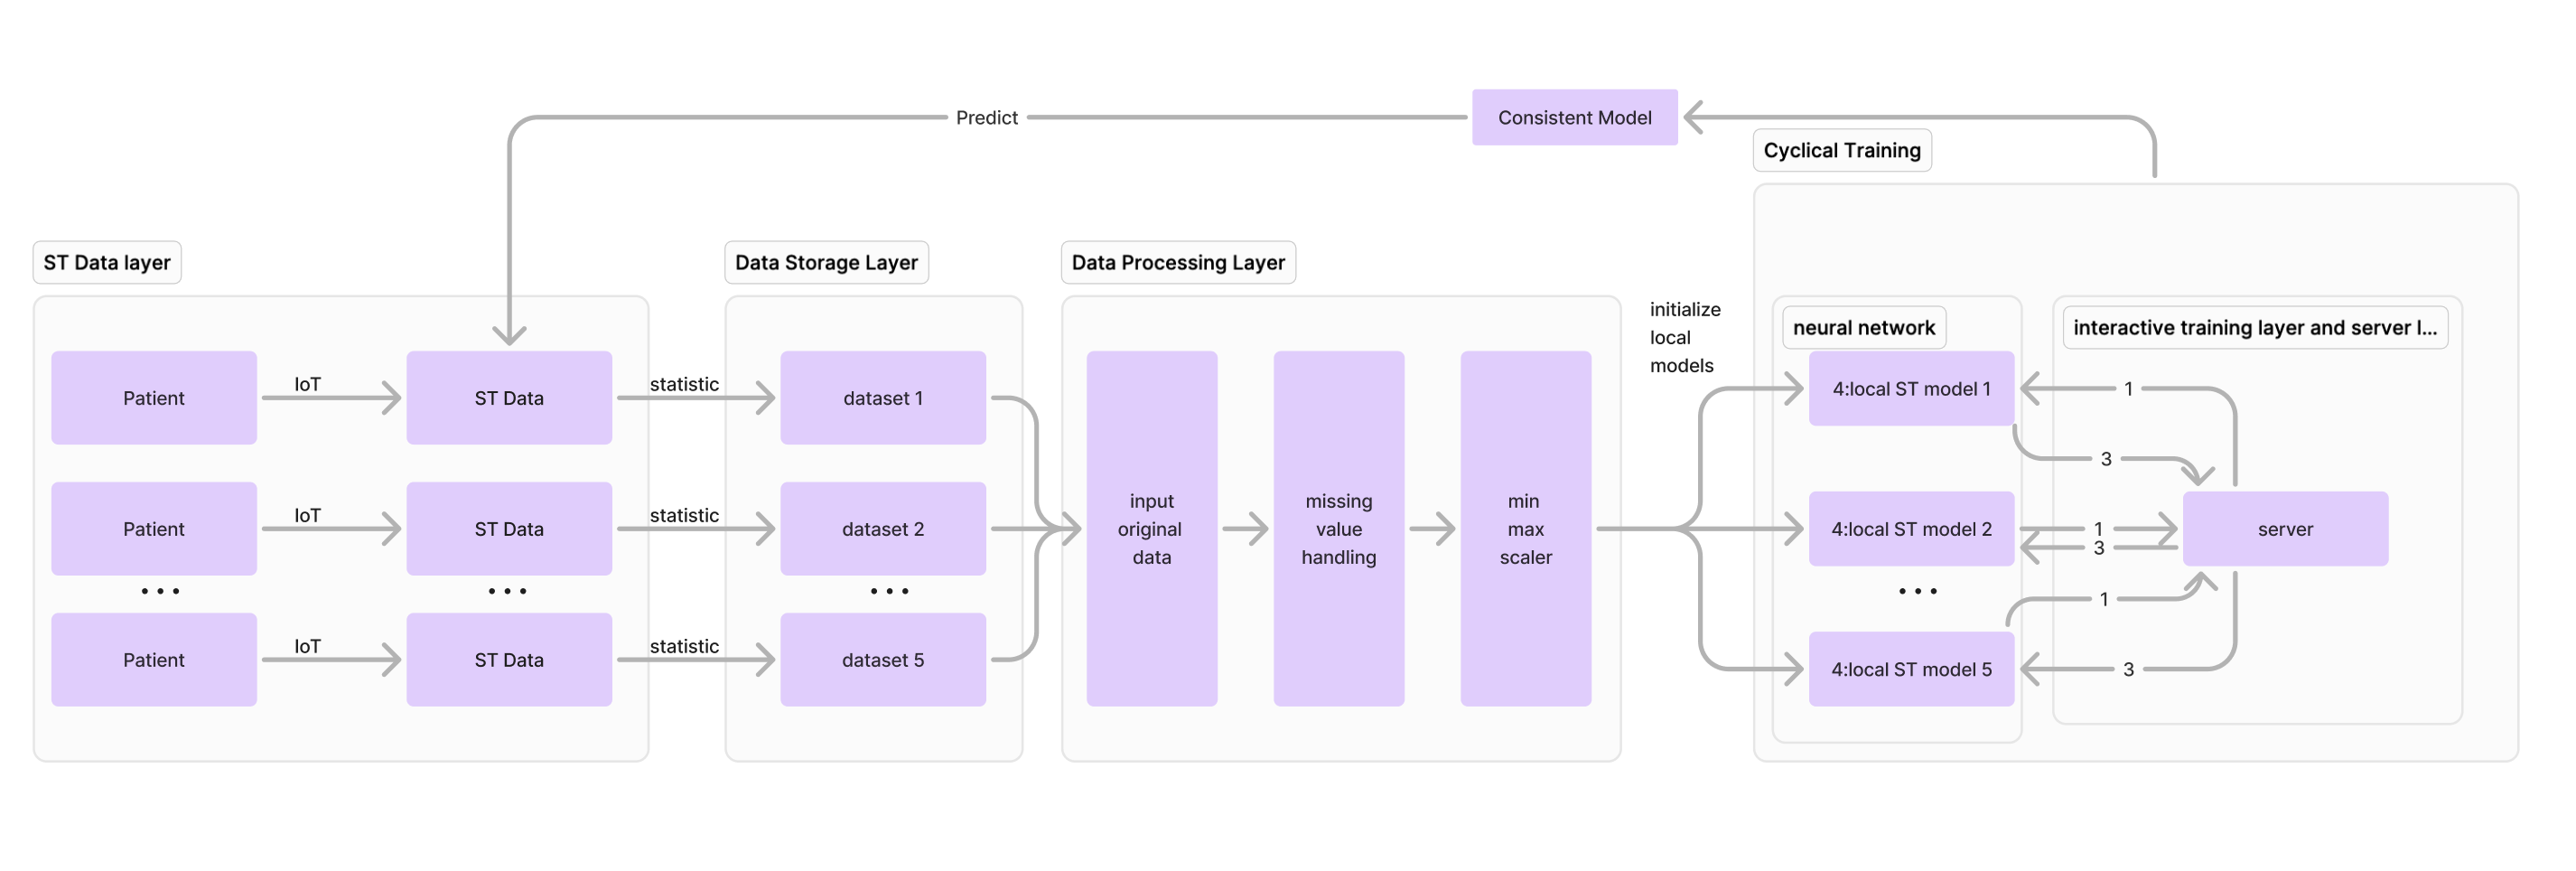
\includegraphics[width=\linewidth]{Screenshot 2025-02-28 at 10.53.33 AM.png} \caption{A general architecture for federated learning of spatiotemporal models in digital health: distributed institutions encode local spatiotemporal patient data, train a shared model on their private cohorts, and exchange only encrypted updates with a central aggregator that synchronizes the per-patient digital twins.} \Description{A general architecture of federated learning for spatiotemporal models in digital health, showing distributed data sources and collaborative training without sharing raw data.} \label{fig:architecture of FL} \end{figure}

\subsection{Visualization in Digital Twin}

Digital Twins provide a method to create highly dynamic and personalized visualizations. They have assisted surgeons through the use of computer-generated vitals and other basic information about the state of the patient. A feedback screen has been used in a virtual space alongside the area of operation to make it easier for a surgeon to split their attention between the two and enhance operational ergonomics \cite{RN137}. But when combined with extended reality, it can also be used to assist with the surgery itself by highlighting areas of operations and showing an example cut line for precise incisions \cite{QUESADAOLARTE20221580}.

Research has also been done that shows that using artificial intelligence (AI) along with digital twins can help generate live data-driven analysis and predictions \cite{RN138}. AI-powered DTs can process the inputted data with little assumptions and output details graphical representations of patient data. This can be brought to the surgery room to help assist the operator and their assistants and keep a check on the patient's status. Outside of surgery, this quick analysis can be applied to clinical check-ups and other health meetings. The use of a general case patient DT that gets modified by generational and previous health conditions of a patient could offer knowledge about a patient's future during their meeting.

Digital twins and extended reality lend themselves well to preplanning for surgeries. The use of AR to display images of CT scans to assist and guide the surgeon has already been documented \cite{RN139}. Pre-generating information for the assistance of the surgeon using the DT could help surgeons have additional help during the procedures while the demand on processing power for that level of analysis would be extended over a longer period. The use of a virtual world also allows manual notes to be made before the surgery. In a paper by \textit{Quesada-Olarte et al.}, a team of surgeons made a 3D mapping of the area of operation before the surgery and highlighted the location of the incision they had to make along with other information. This allowed them to go into the surgery with it already mapped out for them and reduce the time of the surgery by a noticeable amount \cite{RN137}.

The use of xR and DTs to present information in a more digestible way for patients that lack a medical background is also a promising use case of predeveloped virtual presentations. In a paper by \textit{Louis et al.}, they created virtual models of patients brains for doctors to use when explaining to patients and provided them with VR equipment. They found an about 25\% increase in positive results for the Results of Corresponding Patient Satisfaction Measures compared to the HCAHPS national average with their result averaged over 257 different patients \cite{RN140}.

Digital twins offer an ideal way to visualize a patient’s dietary health throughout time. \textit{Gkouskou et al} proposes the idea of using digital twins to create snapshots of a patient's nutritional health throughout their life. They introduced how longitudinal metabolomic, immune, behavioral, and gut microbial parameters would be incorporated into these digital twins that capture a patient throughout time. This method of visualization feeds into a longitudinal spatiotemporal model by using the data on a patient through time and space to create a digital twin that models their nutritional health \cite{gkouskou2020virtual}.

\section{World Model Based Digital Twins in Digital Health}
\label{sec:world_model_dt}
World model based digital twins represent a more active form of patient-centered digital twin system. A conventional spatiotemporal model usually learns a mapping from historical observations to future outcomes, while a world model learns a compact latent state and a transition mechanism that can be rolled forward under hypothetical actions. When this model is synchronized with a medical digital twin, multimodal observations from electronic health records, wearable signals, imaging, mobility traces, environmental exposures, and lifestyle records can be compressed into an evolving patient state. The resulting system can then estimate plausible future trajectories under alternative interventions, making world models a bridge between spatiotemporal representation learning, personalized digital twins, and clinical decision planning \cite{Zheng2026DTtoWM}.

\subsection{Patient-State Simulation and Counterfactual Planning}
The central contribution of a health world model is the ability to simulate patient-state evolution rather than only predict a single endpoint. In this setting, the model receives a latent representation of the current patient state and an action or intervention, such as medication adjustment, dietary change, rehabilitation scheduling, sleep modification, or exposure reduction. It then produces a short- or long-horizon trajectory describing how relevant physiological, behavioral, or clinical variables may evolve. This counterfactual capability is especially valuable for chronic disease management, where clinicians often need to compare multiple plausible intervention paths before selecting a treatment strategy.

Unlike generic generative models, world model--based digital twins must remain anchored to a specific patient. The digital twin supplies continual synchronization: new observations update the latent state, correct outdated assumptions, and constrain future rollouts. Spatiotemporal learning supplies the representation backbone by encoding temporal dynamics and spatial context, including regional exposures, organ-level imaging structures, mobility environments, and patient-specific behavioral patterns. Together, these components allow the system to move from passive monitoring toward active scenario testing while keeping clinicians responsible for final interpretation and intervention selection.

\subsection{Layered Architecture for Spatiotemporal World Models}
An integrated architecture can be organized into three interacting layers. First, spatiotemporal representation models learn structured embeddings from multimodal longitudinal data, including physiological time series, mobility traces, imaging sequences, dietary records, and environmental exposures. Second, the digital twin layer maintains synchronization between these representations and the individual patient through continual updating, data quality checks, and patient-specific calibration. Third, the world model layer operates on the twin's latent patient state to generate action-conditioned rollouts under candidate interventions. This third layer extends the twin from a monitoring and prediction tool into a simulation and planning environment, while still requiring human-in-the-loop review for clinically meaningful decisions \cite{Sadee2025MedicalDT}.

This layered structure also clarifies why world models should not be treated as an isolated algorithmic module. Their reliability depends on the upstream quality of multimodal data fusion, temporal alignment, missing-data handling, and personalization. Their usability depends on downstream interfaces that present intervention assumptions, predicted trajectories, and uncertainty in ways clinicians and patients can understand. Therefore, a world model based digital twin should be evaluated as a coupled system that includes data ingestion, representation learning, simulation, uncertainty estimation, visualization, and clinical workflow integration.

\subsection{Verification, Validation, and Uncertainty}
Verification, validation, and uncertainty quantification are particularly important for world model based digital twins because simulated intervention trajectories can influence real clinical decisions. Verification asks whether the implemented model behaves as intended: data pipelines should preserve temporal order, action labels should correspond to clinically meaningful interventions, constraints should prevent physiologically impossible states, and rollout code should be reproducible across software and hardware environments. For medical use, verification should also include stress tests for missing values, delayed sensor streams, corrupted measurements, and distribution shifts across institutions or devices.

Validation asks whether the simulated trajectories are clinically credible. Retrospective validation can compare model rollouts with held-out patient histories, but this is not sufficient because many candidate interventions are counterfactual and cannot be directly observed in the same patient. Stronger validation should include calibration across rollout horizons, subgroup performance analysis, comparison with mechanistic clinical knowledge, external validation on independent cohorts, and eventually prospective studies in which predictions are assessed before outcomes are known. Evaluation should move beyond short-horizon predictive discrimination and include whether the model ranks intervention options consistently with clinical evidence, whether it identifies unsafe trajectories, and whether its recommendations remain stable under small perturbations of noisy inputs.

Uncertainty grows as rollouts extend into the future. Action-conditioned simulation introduces error accumulation, hidden confounding in observed treatment decisions, partial observability of patient states, and ambiguity when multiple future trajectories are plausible. A clinically useful system should therefore report calibrated uncertainty intervals, separate aleatoric uncertainty from epistemic uncertainty where possible, detect out-of-distribution states, and communicate when no reliable recommendation can be made. These safeguards are essential if digital twins are to evolve into trusted world model based decision support systems rather than opaque simulators \cite{Sel2025VVUQ}.


\section{Future Prospects of Digital Twin with Spatiotemporal Models in Digital Health Field}
\label{sec:future}
As deep neural networks (DNNs) continue to advance, their application in Spatiotemporal data modeling is becoming increasingly sophisticated. Future developments will likely focus on integrating multimodal data sources, enhancing model efficiency through parallel computing, and improving interpretability for better decision making. Privacy concerns will also drive innovations in secure learning mechanisms, ensuring sensitive information is protected while maximizing collaborative research potential. This chapter explores the key directions in Spatiotemporal model research and their implications for various fields.
\paragraph{The Value of Digital Twin and Spatiotemporal Modeling in Digital Health}

Modern healthcare faces multiple challenges, including fragmented health data, delayed diagnosis, limited personalization, and inefficient use of medical resources. One of the key issues is the lack of high quality, continuous, and comprehensive medical data, which restricts the development of accurate and generalizable AI models. Digital Twin technology, when combined with Spatiotemporal modeling, offers a promising solution to these challenges. Digital Twins create dynamic, real-time virtual representations of patients or systems, continuously updated through multi-source data such as wearable devices, clinical records, environmental sensors, and mobility data. Spatiotemporal models can then learn from these rich data streams to simulate health trends, forecast disease progression, and support real-time clinical decisions. Importantly, Digital Twins help address the medical data gap by continuously generating high-resolution, temporally aligned data. This not only improves personalized care but also supports the creation of more robust and generalizable Spatiotemporal models \cite{ali2024spatialtwins}. In the future, with wider adoption of Digital Twin systems, the accumulation of diverse and high-quality datasets will likely lead to the emergence of standardized models that can be applied across populations and scenarios \cite{bilal2025cityseircast}.

\paragraph{Exploration of Spatiotemporal Models and Technological Advancements}

Spatiotemporal models in dietary interventions, diabetes management, depression research, and cardiac disease analysis demonstrate diverse technical approaches and significant potential, ranging from video-based behavioral studies to multi-source time-series prediction and graph-based modeling of brain networks and cardiac electrophysiology. Despite variations in data types, downstream tasks, and neural network architectures, deep learning consistently shows advantages in capturing Spatiotemporal dependencies and integrating multimodal information. With the continuous development of big data, cloud computing, and high-performance parallel computing, researchers are increasingly able to process massive datasets efficiently by leveraging distributed architectures and advanced computing platforms, while incorporating graph networks, deep neural networks, and multimodal fusion methods to more effectively capture temporal and spatial dependencies. However, these advancements also highlight key challenges: limited data availability and quality, stringent requirements for privacy protection and cross-center collaboration, insufficient exploration of multimodal fusion, and constraints on real-time performance and model generalization. In this context, privacy-preserving technologies such as federated learning and differential privacy are essential to balance sensitive information security with collaborative multi-party data usage. Looking ahead, as wearable devices and large-scale medical data become increasingly widespread, and as self-supervised learning, physics-informed constraints, and edge computing mature, Spatiotemporal models are likely to become even more valuable in digital health. Nevertheless, unlocking their widespread clinical adoption will require continued efforts to establish standardized protocols, ensure robust data protection, develop reliable models, and achieve tighter integration with real-world healthcare workflows.
\paragraph{Promoting Data Sharing in Digital Health Research}
Digital health research requires the integration of heterogeneous data from hospitals, wearable devices, environmental sensors, and genomic sequencing. Establishing standardized data collection, annotation, and exchange protocols is essential to achieving large-scale data sharing. As privacy protection and ethical compliance become increasingly significant, technologies such as federated learning and secure multi-party computation provide feasible solutions for data sharing, allowing institutions to maintain data autonomy while still collaborating on model training and generating high-accuracy analytical models. Only with joint advancements in technology and legal frameworks can digital health research overcome data silos, ultimately enabling more precise disease monitoring, health interventions, and medical services.

\paragraph{From Clinical Trials to Real World Commercial Applications}
Translating Spatiotemporal data technologies from laboratories to market applications necessitates ensuring model stability and scalability in complex and dynamic real-world scenarios. This requires maintaining high accuracy while balancing computational costs, data security, and user experience. In the field of digital health, this transition involves not only moving from highly controlled clinical trials to large-scale population applications but also fostering collaboration with insurance companies, pharmaceutical enterprises, and hospitals to establish a sustainable commercialization ecosystem. Technology providers must continuously refine their products based on different application scenarios, collect and respond to user feedback, and drive rapid iteration and innovation. Only by doing so can Spatiotemporal data-driven solutions take root in the industry and achieve widespread adoption.

\paragraph{Future World Model Based Digital Twins}
Future digital health systems are likely to benefit most from constrained world models that are synchronized through digital twins and informed by spatiotemporal context. In such systems, multimodal patient data can be compressed into latent health states, updated continually as new observations arrive, and rolled forward under candidate interventions to estimate plausible future trajectories. The key research challenge is to combine the adaptability and generative capacity of world models with the personalization, synchronization, and accountability required of medical digital twins. Progress will depend on hybrid mechanistic learning architectures, multiscale representations spanning organ, person, and environment level dynamics, privacy-preserving continual learning, and rigorous prospective validation before deployment in clinical workflows.\cite{DeDomenico2025ComplexSystems}
% \bibliographystyle{ieeetr}  % Default numerical style
% \bibliographystyle{ACM-Reference-Format} 
\bibliographystyle{unsrtnat}
\bibliography{newST}
\end{document}

\endinput
%%
%% End of file `sample-acmcp.tex'.
